\documentclass[10pt]{article}
%==========================================================================================

\usepackage[utf8]{inputenc}
\usepackage[brazil]{babel}
\usepackage[T1]{fontenc}
\usepackage{amsmath}
\usepackage{amsfonts}
\usepackage{mathrsfs}
\usepackage{amssymb}
\usepackage{graphicx}
\usepackage{geometry, calc, color, setspace}
\usepackage{indentfirst}
\usepackage{wrapfig}
\usepackage{boxedminipage}
\usepackage{enumerate}
\usepackage{float}
\usepackage{paralist}
\usepackage{comment}
\usepackage{icomma}
\usepackage{rotating}
\usepackage{multirow}
\usepackage[position=bottom]{subfig}
\usepackage{array}
\usepackage{tabularx}
\usepackage{float}
\usepackage{array}

\newcolumntype{L}[1]{>{\raggedright\let\newline\\\arraybackslash\hspace{0pt}}m{#1}}
\newcolumntype{C}[1]{>{\centering\let\newline\\\arraybackslash\hspace{0pt}}m{#1}}
%\newcolumntype{R}[1]{>{\raggedleft\let\newline\\\arraybackslash\hspace{0pt}}m{#1}}
\newcolumntype{R}{>{\raggedleft\let\newline\\\arraybackslash\hspace{0pt}}X}

\usepackage[alf,bibjustif]{abntex2cite}
%\usepackage{abntcite}

% Para o alinhamento dos títulos das figuras
\usepackage{caption}
%\captionsetup[figure]{format=hang,labelsep=endash,font=small,justification=RaggedRight,singlelinecheck=off, margin=1cm}
\captionsetup[subfigure]{textfont=small,singlelinecheck=off,justification=raggedright}


%%  Inserindo os códigos Python ==================================
\usepackage{listings}

%\definecolor{light_gray}{rgb}{0.97,0.97,0.97}
%\definecolor{mymauve}{rgb}{0.58,0,0.82}
%\definecolor{mygreen}{rgb}{0,0.6,0}

\lstset{
  language = Python,
  inputencoding = utf8,
  backgroundcolor = \color{white},
  columns=fullflexible,
  basicstyle=\ttfamily,
  breaklines=true,
  postbreak=\raisebox{0ex}[0ex][0ex]{\color{black}$\hookrightarrow$\space},
  keywordstyle=\color{black},      % keyword style
  stringstyle=\color{black},
  commentstyle=\color{black}
}

\newcommand{\HRule}{\noindent\rule{\linewidth}{0.2mm}}

\usepackage{mathpazo}                         % tem suporte matemático
\usepackage[scaled=0.85]{beramono}            % usa esta nos verbatins [scaled=0.9]

\renewcommand\UrlFont{\color{black}\rmfamily} 

\def\distnumber{2.3em}

%==========================================================================================

\author{Walef Machado de Mendonça\footnote{Mestrando em Estatística Aplicada e Biometria na Universidade Federal de Alfenas}\\
Patrícia de Siqueira Ramos\footnote{Professora da Universidade Federal de Alfenas, campus Varginha}}

%==========================================================================================


\title{O seguro rural no Brasil: evolução e distribuição regional}

\date{}

\begin{document}

\maketitle

\begin{abstract}
As atividades agropecuárias se inserem em um contexto de adversidades que as colocam em situação diferenciada em relação aos riscos enfrentados pelos produtores. Tais atividades demandam grandes investimentos, o que faz com que sua atratividade esteja relacionada às formas existentes de gerenciamento de riscos. Uma das formas mais usuais de gerenciamento de risco neste setor é a contratação de Seguro Rural, uma vez que esta modalidade de seguro possibilita a recuperação da capacidade financeira do produtor na ocorrência de sinistros. Nesse sentido, o objetivo do trabalho é avaliar a distribuição e a dinâmica espacial de variáveis relacionadas às apólices de Seguro Rural contratadas nos municípios brasileiros no período de 2006 a 2019. Além disso, busca-se investigar a existência de dependência espacial e a presença de agrupamentos com grande número de apólices de Seguro Rural. Para tanto, utiliza-se os dados dos Censos do Seguro Rural, compilados pelo Ministério da Agricultura, Pecuária e Abastecimento (MAPA) e Análise Exploratória de Dados Espaciais (AEDE). Os resultados apontam que as maiores concentrações de apólices de Seguro Rural estão situadas nas regiões Sul e Centro-Oeste. Além disso, apesar de haver um aumento nas contratações de Seguro Rural, há também uma tendência de maior concentração espacial das apólices ao longo do período analisado. \\
\newline
\noindent {\textbf{Palavras-chave}}: Seguro rural. Política agrícola. Estatística espacial. Autocorrelação espacial. I de Moran.
\end{abstract}

\section{INTRODUÇÃO}

O setor agropecuário brasileiro tem se destacado nas últimas décadas por seu crescimento proveniente da aplicação de novas tecnologias ao clima tropical e a incorporação de novas áreas de terras \cite{brasil19a}. Segundo dados dos censos agropecuários, entre $2006$ e $2017$, tanto a área total quanto a produção agrícola e pecuária vivenciaram crescimento. Neste período houve um acréscimo de cerca de $5,8\%$ na área total dos estabelecimentos agropecuários \cite{ibge19}. Com relação à sua participação no PIB, em 2019, a parcela do agronegócio brasileiro foi de  $20,5\%$  do PIB nacional. Já em 2020, o setor agropecuário brasileiro alcançou a participação de $26,6\%$ do PIB. Em valores monetários, o PIB do País totalizou R\$ $7,45$ trilhões em 2020, e a participação do agronegócio chegou a quase R\$ $2$ trilhões \cite{cepea21}. 

Dada a relevância do setor agropecuário na economia brasileira, é necessário destacar que este ramo apresenta características muito específicas com relação à magnitude dos riscos aos quais está sujeito \cite{burgo05}. Alguns riscos mais relevantes se devem, principalmente, às instabilidades climáticas e ameaças sanitárias, que podem afetar a produção, ou à razões de mercado, como variações das taxas de câmbio e juros, ou a condições ligadas ao ambiente de negócios, tais como, alterações em marcos regulatórios e em políticas públicas. Todos esses fatores geram variações na renda do setor, que devem ser enfrentadas por meio de políticas de apoio à gestão de riscos \cite{brasil21}. 

Uma gestão de riscos apropriada tem potencial de afetar de forma positiva a estabilidade da renda do produtor e sua própria permanência no setor agropecuário. O gerenciamento de riscos agropecuários pode ocorrer de diversas maneiras, no entanto, a contratação de seguro é uma das medidas mais comuns. O seguro rural é uma importante ferramenta de mitigação de riscos e proteção da renda. Esta modalidade de seguro atua no sentido de amenizar as perdas e possibilitar a recuperação da capacidade financeira do produtor rural em caso de ocorrência de sinistros \cite{brasil19b}. 

Nesse sentido, o presente trabalho tem por objetivo, avaliar a distribuição espacial do seguro rural nos municípios brasileiros entre 2006 e 2019. Para tanto, busca-se investigar se, no Brasil, as variáveis de seguro rural se distribuem de forma aleatória no espaço ou se há padrões de distribuição espacial. Além disso, através da análise da distribuição espacial do seguro rural no período, busca-se identificar se há regiões que tiveram alterações significativas no número de contratações de seguro. Por fim, este estudo busca fornecer informações para o debate de aperfeiçoamentos no sistema de seguro rural brasileiro, de forma a contribuir para uma agricultura mais eficiente e com menores riscos para o produtor rural.

O trabalho está estruturado da seguinte forma: a próxima seção apresenta uma breve revisão de literatura sobre o seguro rural. A terceira seção apresenta os dados, os procedimentos de análise e recursos computacionais que serão utilizados. A quarta seção apresenta resultados e discussões. A última seção apresenta as considerações finais.

\section{UM PANORAMA DO SEGURO RURAL NO BRASIL}

No Brasil, as primeiras iniciativas de se instalar um sistema de seguro rural remontam à meados da década de $1930$ e desenvolveram-se principalmente nas esferas estaduais. Em $1939$, o Estado de São Paulo determinou a criação de um seguro obrigatório contra o granizo na produção de algodão \cite{maia11}. Segundo Silva, Teixeira e Santos (2014), os resultados do seguro para a proteção da lavoura algodoeira em São Paulo influenciaram a criação de novos programas como a Carteira de Seguro Agrícola contra Granizo para a Viticultura, criada em $1948$, e a Carteira de Seguro Agrícola contra Geada para Horticultura instituída em $1964$.

Além disso, Silva, Teixeira e Santos (2014) apontam em seu trabalho o seguro para granizo que foi criado no final da década de $1940$ no Instituto Rio-Grandense do Arroz (Irga), e o seguro criado pela Associação dos Fumicultores do Brasil (Afubra), que objetivava ressarcir com recursos próprios os produtores de fumo nos estados de Santa Catarina e Rio Grande do Sul.

Já no âmbito nacional, foi criado em $1948$, o Instituto de  Resseguros do Brasil (IRB), com o objetivo de reduzir os prejuízos de eventos adversos e assegurar uma maior estabilidade aos produtores rurais \cite{silva14}. Além disso, o Governo Federal criou, em $1954$, a Companhia Nacional de Seguro Agrícola (CNSA) e o Fundo de Estabilidade do Seguro Agrário. Para mais, Maia,  Roitman e de Conti (2011) evidenciaram que a estruturação e gestão dos seguros da CNSA ficaram, de início, sob responsabilidade do IRB. No entanto, segundo Gemignani (2000), as atividades da CNSA se encerraram em $1996$, em decorrência do insucesso em disseminar a adesão ao seguro rural de forma a possibilitar sua viabilidade econômica \cite{maia11, silva14}.

Na segunda metade da década de $1960$, são instituídos o Decreto-Lei nº $73$ ($1966$) e o Decreto nº $60.459$ ($1967$), que instituem os fundamentos institucionais para as atividades de seguro e a criação do Sistema Nacional de Seguros Privados (SNSP). O decreto de $1967$ também criou o Fundo de Estabilidade do Seguro Rural (FESR), cujos recursos inicialmente eram geridos pelo IRB e cujo objetivo principal era garantir a equilíbrio do sistema de seguro rural e fornecer uma cobertura adicional para os riscos de sinistro \cite{silva14}

% Até aqui Ok
Instituída em $1970$, a Resolução nº $5$ do Conselho Nacional de Seguros Privados teve uma função relevante na caracterização das modalidades de seguros agrários. Nesta Resolução, foi definido o seguro agrícola, que fornece cobertura contra perdas decorrentes de fenômenos meteorológicos, doenças e pragas, o seguro pecuário que fornece cobertura para morte de animais causadas por doenças ou acidentes, assim como, o seguro de benfeitorias e produtos agropecuários. Em suma, a Resolução nº $5$ também estabelece o seguro de crédito, que cobre incapacidade de pagamento de compradores dos produtos agropecuários \cite{silva14}.

A criação do Programa de Garantia da Atividade Agropecuária (Proagro), através da Lei nº $5.969$, de $11$ de dezembro de $1973$ ocorreu devido ao fato de que, apesar das diversas ações do Governo Federal, o seguro rural se desenvolveu de forma lenta e restrita à uma pequena parcela da produção \cite{silva14}. O Proagro inicialmente ficou sob a responsabilidade do Banco Central e passou a vincular o seguro rural às operações de crédito agropecuário. Por sua vez, o Banco Central utilizou emissões monetárias para pagamentos de sinistros. Segundo Maia, Roitman e De Conti (2011), o sistema de financiamento do Proagro gerou déficits que provocaram diversas alterações no Programa, que ainda permanece um dos mais importantes instrumentos para a gestão de riscos na agricultura no Brasil.

Instituído por meio da Lei nº $10.823$ de $19$ de dezembro de $2003$ e do Decreto nº $5.121$ de $2004$, o Programa de Subvenção ao Prêmio do Seguro Rural (PSR), passou a ser a política adotada pelo Governo Federal para o estímulo ao sistema de seguro rural no Brasil \cite{brasil18}. O PSR busca, assim como ocorre em países europeus e nos Estados Unidos, conceder subvenção econômica ao valor do prêmio do seguro rural contratado com seguradoras autorizadas \cite{maia11, silva14}.

Dessa forma, o PSR tem como finalidade subsidiar parte do prêmio do seguro rural, de modo a assegurar a responsabilidade do seguro rural como forma de garantir a estabilidade da renda do produtor, além de suscitar o aplicação das tecnologias adequadas para os empreendimentos agropecuários \cite{guia_20}. Tal política do governo busca tornar o seguro rural mais acessível aos agricultores, dividindo os custos de aquisição da apólice entre o governo e os produtores. 


\section{MATERIAL E MÉTODOS}\label{material_e_metodos}

%O objetivo dessa seção é apresentar os dados utilizados no trabalho, descrever a metodologia e os recursos computacionais utilizados na presente análise.

\subsection{DADOS}

% Fonte dos Dados 

Os dados de seguro rural utilizados neste trabalho foram obtidos no endereço eletrônico do Ministério da Agricultura, Pecuária e Abastecimento (MAPA) \cite{brasil21}. Foram utilizados dados com valores anuais a partir do ano de $2006$ até o ano de $2019$ (último ano disponível até então) para os dados municipais. Os dados agregados são provenientes do Atlas do Seguro Rural do MAPA e apresentam periodicidade anual a partir do ano de $2006$. Também foram utilizados dados que contém atributos geográficos, como a posição e o formato, do território brasileiro. Esses dados estão disponíveis no endereço eletrônico do Instituto Brasileiro de Geografia e Estatística \cite{ibge20}.

O conjunto de dados de seguro rural possui informação referente à localização geográfica da contratação do seguro rural. No entanto, foram detectadas algumas divergências relacionadas a distritos ou outras localidades, como fazendas e vilarejos, que foram apontados como o local referente à contratação do seguro. 

Para corrigir essas divergências, de forma a ter informações referentes apenas aos municípios brasileiros, as informações relacionadas às demais localidades foram acrescentadas aos municípios correspondentes. Para a identificação, foi feita uma busca de cada localidade que não tinha correspondência com os municípios brasileiros. Essa busca foi feita inicialmente no site \textit{google maps}, contendo, como termo de busca, o nome da localidade e o seu estado \footnote{Foi considerado que a informação referente aos Estados estava correta nos dados do MAPA}. Nos casos em que a informação do município ao qual a localidade pertencia estava disponível no resultado da pesquisa, o nome do município era utilizado em uma segunda busca no site \textit{Portal Cidades} do IBGE \footnote{\url{https://cidades.ibge.gov.br}}. O \textit{Portal Cidades} apresenta, na maioria dos casos, a divisão territorial e administrativa atualizada, de forma a possibilitar a correção das divergências nos dados. Nos casos em que a informação do município ao qual a localidade pertencia não estava disponível no resultado da pesquisa, o nome da localidade era utilizado como termo de busca de CEPs no site dos Correios \footnote{\url{https://buscacepinter.correios.com.br/app/localidade_logradouro/index.php}}. Para os casos em que não foi possível encontrar nenhum resultado com relação ao município correspondente, a localidade em divergência foi atribuída ao município geograficamente mais próximo \footnote{Os códigos utilizados na análise estão disponíveis no \textit{GitHub} e os link estão no Apêndice B.}.

% Editar essa parte!!!!!
%Variáveis total de apólices contratadas (TAC), soma da importância segurada (R\$ milhão) (SIS), soma dos prêmios (R\$ milhão) (SPR), total de subvenção (R\$ milhão) (TSB), soma das indenizações pagas (R\$ milhão) (SIP), taxa média aplicada às apólices (TMA) e número de apólices indenizadas (NAI).

%\subsection{ANÁLISE DOS DADOS} 

%Após uma análise exploratória dos dados, foi realizada a primeira parte da Análise Exploratória de Dados Espaciais (AEDE), onde os dados agregados por municípios serão apresentados por meio de mapas temáticos, de forma a ilustrar o padrão espacial das variáveis de seguro rural. No segundo passo da AEDE, o valor do \textit{I} de Moram global foi calculado e sua significância obtida por meio do pseudo valor-$p$, obtido a partir de $999$ permutações aleatórias. Neste estudo, foi considerado um nível de significância $\alpha = 0,05$. Foi adotada a matriz de pesos espaciais de contiguidade com a convenção rainha, considerando os vizinhos de primeira ordem. Tal matriz foi adotada por ser a mais utilizada na literatura em trabalhos semelhantes \cite{almeida12}. 

%Para a construção da matriz de pesos espaciais, foram retirados os municípios de Fernando de Noronha, que se constitui em um arquipélago pertencente ao estado de Pernambuco, e Ilhabela, arquipélago no litoral norte do estado de São Paulo. Estes municípios foram desconsiderados pois, além de se constituírem de ilhas, não possuem nenhuma apólice de seguro rural contratada durante os anos em análise. Uma vez definida a matriz, se o valor do \textit{I} de Moran global for significativo, a hipótese de aleatoriedade espacial deve ser rejeitada e há evidências de que há uma autocorrelação positiva \cite{almeida12}. 

%O terceiro passo da análise espacial das variáveis de seguro rural consistiu na obtenção dos mapas \textit{LISA}, de forma a identificar padrões locais de autocorrelação espacial e \textit{outliers} espaciais. Esses mapas ilustram cada uma das observações e indicam se seus valores foram considerados significativos em relação à estatística do I de Moran local \cite{almeida12, anselin95}. 

%\subsection{RECURSOS COMPUTACIONAIS}  

Esse estudo foi feito utilizando a linguagem de programação \textit{Python} \cite{python17}, através da interface \textit{Jupyter} \cite{jupyter17} \cite{perez07} \cite{kluyver19}; Além disso, foram utilizadas as seguintes bibliotecas: \textit{Pandas} \cite{mckinney10}, que é uma ferramenta  para análise e manipulação de dados; \textit{NumPy} \cite{walt11}, que é destinado a possibilitar a computação numérica com \textit{Python}; \textit{SciPy} (JONES et al., 2001); % rever essa citação 
\textit{Matplotlib} \cite{hunter07} e \textit{Seaborn} \cite{waskom14}, que são bibliotecas para criar visualizações  de dados em \textit{Python}; \textit{jenkspy}, para a utilização do algoritmo Fisher Jenks \cite{jenks77} e \textit{Geopandas} \cite{jordahl14}, que possibilita a construção dos mapas. 

\section{RESULTADOS E DISCUSSÃO}

\subsection{A EVOLUÇÃO DO SEGURO RURAL} 

Inicialmente, serão apresentados dados ilustrativos da trajetória do Seguro Rural no Brasil. Serão analisados dados anuais referentes ao número de apólices contratadas, ao número de apólices indenizadas, aos valores de subvenção, indenização e prêmio. Também serão apresentados dados referentes à participação das seguradoras e das principais culturas no número de apólices contratadas. Foram utilizados dados da Plataforma Atlas do Seguro Rural. É importante destacar que os valores referentes ao ano de $2021$ ainda não estavam consolidados na data do presente estudo.

%\subsubsection{Apólices contratadas}

Nesta seção, serão analisados dados anuais referentes às apólices de seguro rural contratadas e os respectivos valores de prêmio e subvenção. 

No gráfico da Figura \ref{apolices_produtores}, é possível observar a evolução do número de produtores e do número de apólices de seguro rural contratadas no período de $2006$ a $2020$. Durante o período analisado, cada produtor contratou, em média, $1,48$ apólices de seguro rural. O número de apólices contratadas tem um crescimento de cerca de $8,69$ vezes durante o período. Entre os anos $2014$ e $2015$, ocorre uma queda de $66,08\%$ nas apólices contratadas. Por sua vez, o número de produtores cresceu $6,36$ vezes entre $2006$ e $2020$.

\begin{figure}[H]
	\centering
	\caption{Número de produtores e apólices de seguro rural contratadas. Brasil $2006 - 2020$}
	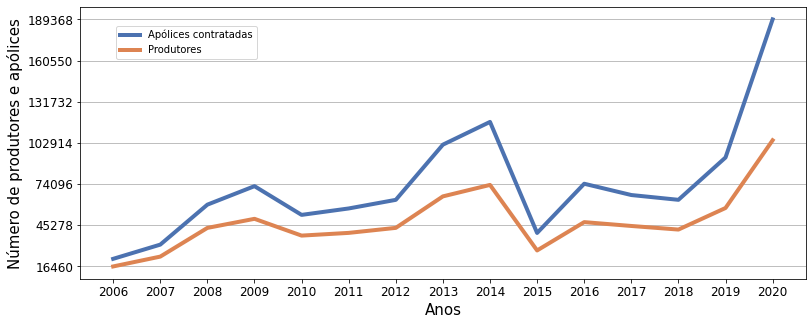
\includegraphics[width=0.8\textwidth]{figuras/apolices_produtores.png}\\
	%\small \textsuperscript {Fonte: Elaboração própria a partir de dados da Plataforma Atlas do Seguro Rural \cite{brasil21b}.}
    \parbox{\dimexpr\linewidth-3cm}{\raggedright
    \strut \textsuperscript{Fonte: Elaboração própria a partir de dados da Plataforma Atlas do Seguro Rural \cite{brasil21b}.}\strut}
    \label{apolices_produtores}
\end{figure}

É importante destacar que, no ano de $2021$, até o mês de junho, havia $66.928$ apólices contratadas \cite{brasil21}. Apesar do valor ser baixo se comparado ao ano de $2020$ ($189.368$ apólices), já é superior a $56,25\%$ dos anos anteriores. Padrão semelhante se observa com o número de produtores. No ano de $2021$, até o mês de junho haviam sido contabilizados $47.472$ produtores segurados \cite{brasil21b}.

%\subsubsection{Valores do prêmio e de subvenção ao prêmio de seguro rural}

O gráfico da Figura \ref{soma_ano_values} apresenta a evolução dos valores em milhões de reais de subvenção ao prêmio de seguro rural, prêmio pago pelo produtor e prêmio recebido pela seguradora entre $2006$ a $2020$. Observa-se que, com exceção do ano de $2014$, é possível notar uma tendência de crescimento dos valores de subvenção e prêmio pagos no período analisado. No ano de 2014, devido à contenções, o governo federal liberou apenas R\$ $400$ milhões dos R\$ $700$ milhões previstos para subsidiar o seguro rural. Esta contenção dos gastos governamentais pode ser um fator a ser considerado na queda dos valores do seguro rural ocorrida entre os anos de $2014$ e $2015$ \cite{andrade21}.

Em $2021$, até o mês de junho, o valor do prêmio pago à seguradora já havia alcançado R\$$1,25$ bilhões, o quarto maior valor registrado e cerca de $50,59\%$ maior que a média. O prêmio do produtor referente ao período de janeiro a junho de $2021$ já era equivalente a R$\$0,77$ bilhões, valor cerca de $69,67\%$ maior que a média do prêmio de responsabilidade do produtor. O valor concedido na forma de subvenção ao prêmio em $2021$ também é o quarto maior valor registrado, cerca de $25,96\%$ maior que a média dos valores de subvenção concedidos . Além disso, a partir do ano de $2016$, a parcela do prêmio sob responsabilidade do produtor passa a superar a parcela concedida pelo governo na forma de subvenção \cite{brasil21b}.

%\begin{figure}[H]
%	\centering
%	\caption{Valores do prêmio e de subvenção ao prêmio de seguro rural. Brasil $2006 - 2020$}
%	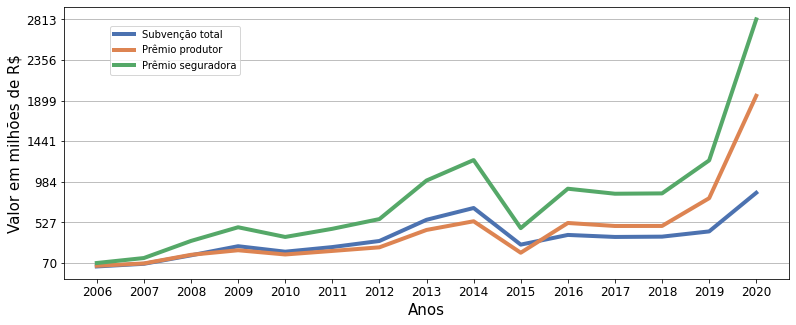
\includegraphics[width=0.8\textwidth]{figuras/soma_ano_values.png}\\
%	\small \textsuperscript {Fonte: Elaboração própria a partir de dados da Plataforma Atlas do Seguro Rural (Mapa, 2021).}
%    \label{soma_ano_values}
%\end{figure}

%\begin{figure}[H]
%	\centering
%	\caption{Soma da importância segurada (R\$ milhões). Brasil $2006 - 2020$}
%	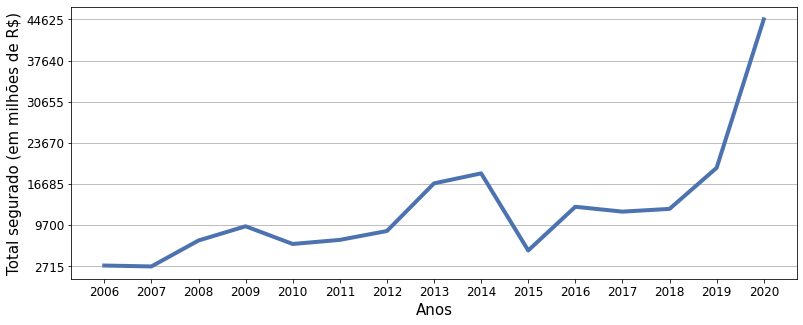
\includegraphics[width=0.8\textwidth]{figuras/total_segurado_mil.png}\\
%	\small \textsuperscript {Fonte: Elaboração própria a partir de dados da Plataforma Atlas do Seguro Rural (Mapa, 2021).}
%    \label{total_segurado_mil}
%\end{figure}

%\begin{figure}[H]
%	\centering
%	\caption{Total da área segurada em hectares. Brasil $2006 - 2020$}
%	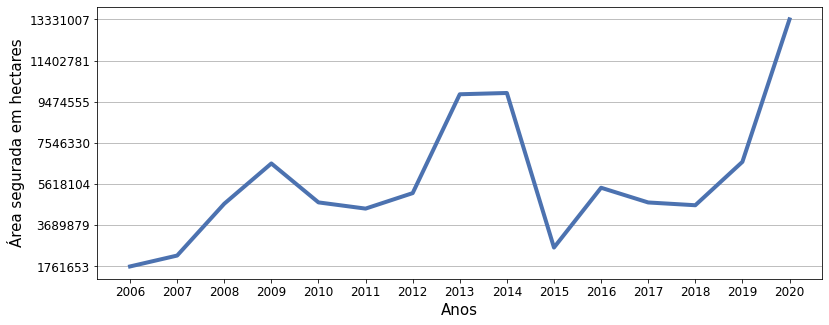
\includegraphics[width=0.8\textwidth]{figuras/area_segurada.png}\\
%	\small \textsuperscript {Fonte: Elaboração própria a partir de dados do Ministério da Agricultura, Pecuária e Abastecimento (MAPA).}
%    \label{area_segurada}
%\end{figure}

%\begin{figure}[H]
%	\centering
%	\caption{Número de apólices de seguro rural indenizadas. Brasil $2006 - 2019$}
%	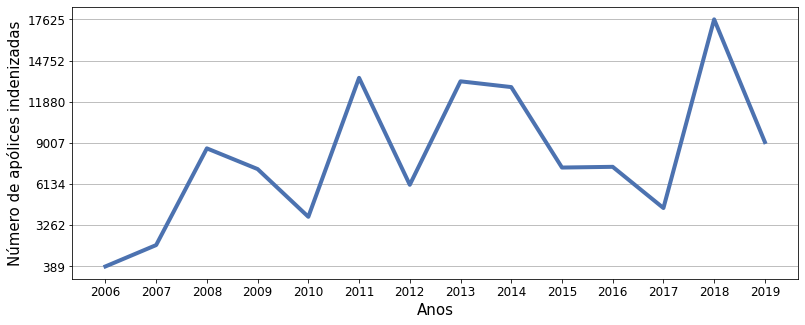
\includegraphics[width=0.8\textwidth]{figuras/apolices_indenizadas.png}\\
%	\small \textsuperscript {Fonte: Elaboração própria a partir de dados do Ministério da Agricultura, Pecuária e Abastecimento (MAPA)}
%    \label{apolices_indenizadas}
%\end{figure}

%\begin{figure}[H]
%	\centering
%	\caption{Valor das indenizações de seguro rural pagas (R\$ milhões). Brasil $2006 - 2019$}
%	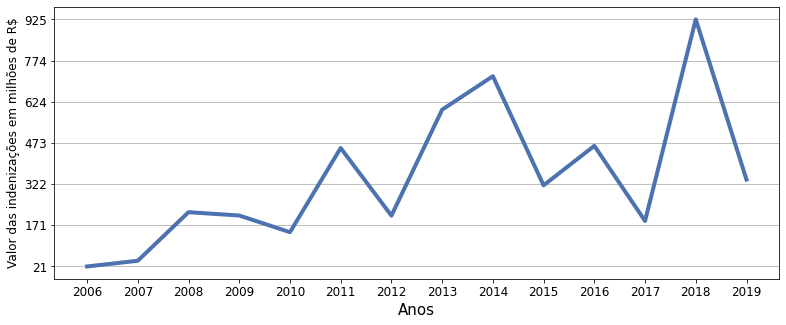
\includegraphics[width=0.8\textwidth]{figuras/valor_indenizacoes.png}\\
%	\small \textsuperscript {Fonte: Elaboração própria a partir de dados do Ministério da Agricultura, Pecuária e Abastecimento (MAPA)}
%    \label{valor_indenizacoes}
%\end{figure}

% variaveis_br
\begin{figure}[H]
	\centering
	\caption{Evolução das variáveis de seguro rural no Brasil}\label{variaveis_br}
	\small
	
	\subfloat[Valores do prêmio e de subvenção ao prêmio de seguro rural\label{soma_ano_values}]{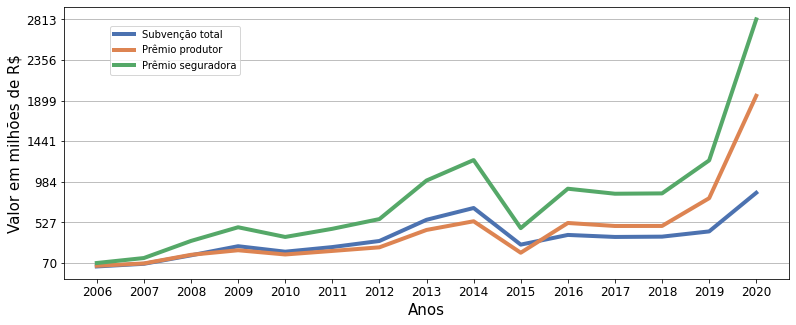
\includegraphics[width=0.45\textwidth]{figuras/soma_ano_values.png}}\hspace{0.1cm}
	\subfloat[Soma da importância segurada (R\$ milhões)\label{total_segurado_mil}]{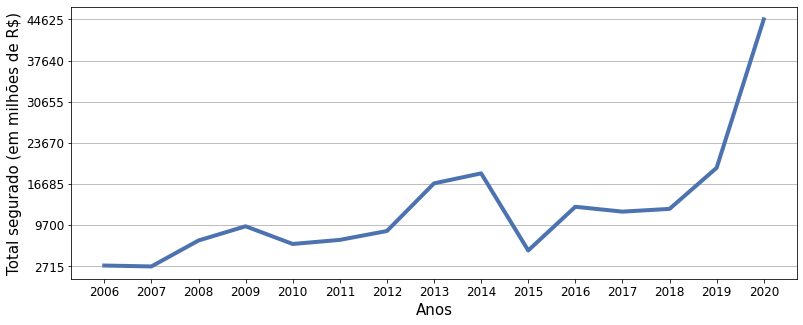
\includegraphics[width=0.45\textwidth]{figuras/total_segurado_mil.png}}\hspace{0.1cm}\\
	
	\subfloat[Total da área segurada em hectares.\label{area_segurada}]{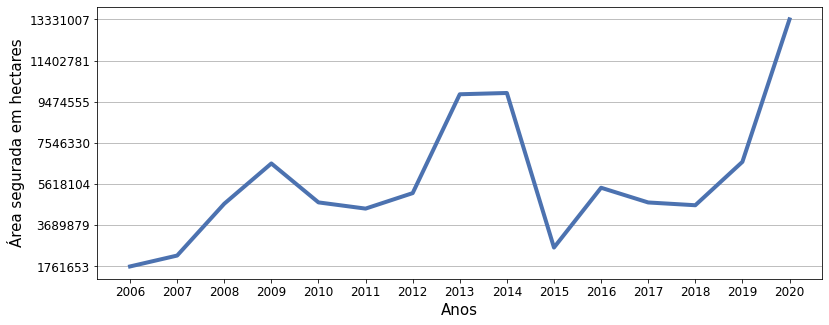
\includegraphics[width=0.45\textwidth]{figuras/area_segurada.png}}\hspace{0.1cm}
	\subfloat[Número de apólices de seguro rural indenizadas\label{apolices_indenizadas}]{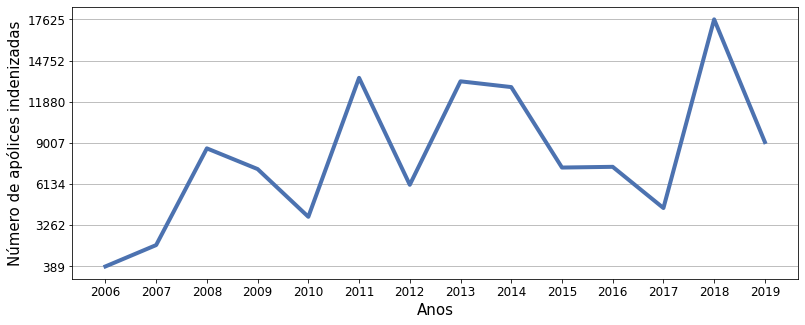
\includegraphics[width=0.45\textwidth]{figuras/apolices_indenizadas.png}}\\
	
	\subfloat[Valor das indenizações de seguro rural pagas (R\$ milhões)\label{valor_indenizacoes}]{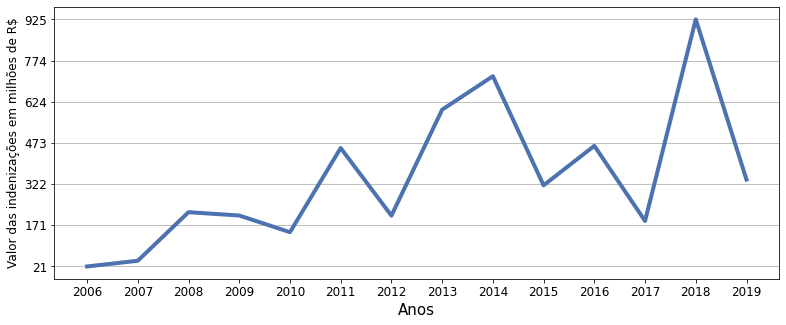
\includegraphics[width=0.45\textwidth]{figuras/valor_indenizacoes.png}}\hspace{0.1cm}
	\subfloat[Taxa média anual de contratação do prêmio de seguro rural\label{taxa_media}]{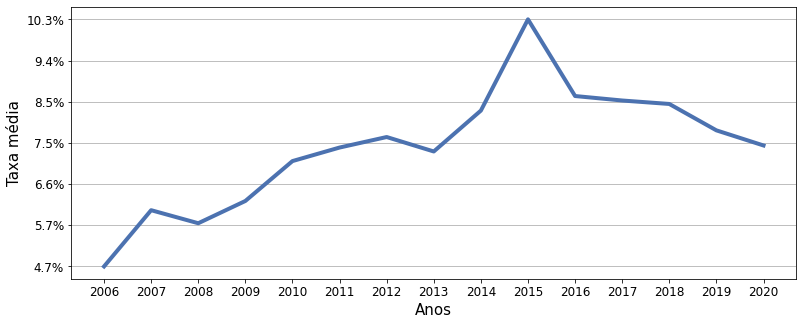
\includegraphics[width=0.45\textwidth]{figuras/taxa_media.png}}
	
	\parbox{\dimexpr\linewidth-2cm}{\raggedright
    \strut \textsuperscript{Fonte: Elaboração própria a partir de dados do Ministério da Agricultura, Pecuária e Abastecimento e da Plataforma
	Atlas do}\strut}\\
    \parbox{\dimexpr\linewidth-2cm}{\raggedright
    \strut \textsuperscript{Seguro Rural \cite{brasil21b}.}\strut}
\end{figure}

Os valores da soma da importância segurada em milhões de reais são apresentados no gráfico da Figura \ref{total_segurado_mil}. Observa-se que há crescimento dos valores segurados, com destaque para o crescimento entre os anos de $2019$ e $2020$, em que o os valores mais que duplicaram. Considerando o período entre $2006$ e $2020$, o crescimento da importância segurada foi de $15,55$ vezes o valor de $2006$. Também é possível observar que, entre os anos de $2014$ e $2015$, ocorreu uma queda de $70,68\%$ do valor segurado.  

Em $2020$, o Programa de Subvenção ao Prêmio do Seguro Rural (PSR) aplicou R\$ $880$ milhões, ou seja, o dobro do valor executado no ano de  $2019$. Para o ano de $2021$, a estimativa apresentada pelo Ministério da Agricultura e Abastecimento foi um aumento de R\$ $1$ bilhão a verba destinada ao PSR \cite{brasil21b}.

No ano de $2014$, o total segurado chegou a R$\$18.462,88$ milhões, no entanto, em $2015$ a soma da importância caiu para R$\$5.398,54$ milhões, o terceiro valor mais baixo do período. O valor mais alto ocorre no ano de $2020$, em que o valor segurado foi de R$\$45,7$ bilhões, o maior desde o início do programa em $2005$.

O valor da importância segurada alcançou $R\$14,4$ bilhões até o mês de junho de $2021$. Este valor é o quinto maior valor da série e já é maior que $25\%$ dos valores registrados nos anos anteriores \cite{brasil21b}. 

%\subsubsection{Área segurada em hectares}

A Figura \ref{area_segurada} apresenta o total da área segurada em hectares nos municípios do Brasil entre os anos de  $2006$ e  $2020$. É possível observar que, a área agrícola segurada no país praticamente dobrou entre $2019$ e $2020$, quando alcançou o maior valor, $13,7$ milhões de hectares, o que representou $20\%$ da área total agrícola do país. O aumento de área em relação a $2019$ é de $98\%$. O maior valor registrado em anos anteriores foi em $2014$, quando foram segurados $9,4$ milhões de hectares. No ano de $2021$, até o mês de junho, foram segurados cerca de $3,76$ milhões de hectares. Esse valor representa cerca de $71,76\%$ da área segurada em $2020$ \cite{brasil21b}. 

%\subsubsection{Indenizações}

Com relação ao número de indenizações,  o gráfico da Figura \ref{apolices_indenizadas} apresenta a evolução das apólices indenizadas ao longo do período analisado. O menor número de indenizações é $389$ em $2006$ e o maior valor ocorreu no ano de $2018$, sendo igual a $17.625$ indenizações. Durante o período, ocorre em média um número de $8.110$ apólices indenizadas por ano, sendo que o crescimento no número de apólices indenizadas foi de $23,31$ vezes entre $2006$ e $2019$. 

Os valores pagos como indenização entre os anos de $2006$ e $2019$ são apresentados no gráfico da Figura \ref{valor_indenizacoes} e variam entre R\$ $20.699.785,74$ em $2006$ e R\$ $924.988.210,45$ em $2018$. A média do valor das indenizações foi de R\$ $345.525.736,50$ no período analisado. 

%\begin{small}
%    \begin{table}[H]
%        \caption{Número de apólices de seguro rural indenizadas por regiões. Brasil $2006-2019$}\label{premio_regioes}
%         \input{../anexos/ap_indeniz_regioes.tex}
%    \end{table}
%\end{small}

%\subsubsection{Taxa média de contratação de seguro rural}

O gráfico apresentado na Figura \ref{taxa_media} mostra a trajetória da taxa de contratação do seguro rural. É possível constatar que a taxa se eleva, em média, de $4,7\%$ em $2006$ para $ 7,46\%$ em $2020$. Até o mês de junho de $2021$, o valor da taxa média havia alcançado $9,79\%$, o segundo maior valor da série, sendo superado pela taxa média cobrada em $2015$, que foi de $10,3\%$ \cite{brasil21b}.  

Segundo Santos e Silva (2017), espera-se que, à medida que o sistema de seguro rural se consolida, reduzam-se os preços das apólices devido aos ganhos de produtividade agropecuária e da redução de fatores de risco. Essas reduções podem ocorrer devido à adoção das orientações do zoneamento agrícola, de um maior conhecimento do histórico de eventos climáticos e dos sinistros ocorridos e, até mesmo em função da adoção de tecnologias, como o uso de irrigação etc. No entanto, essa redução das taxas não ocorreu no período analisado, como observado na Figura \ref{taxa_media}. 

%\begin{figure}[H]
%	\centering
%	\caption{Taxa média anual de contratação do prêmio de seguro rural. Brasil $2006 - 2020$}
%	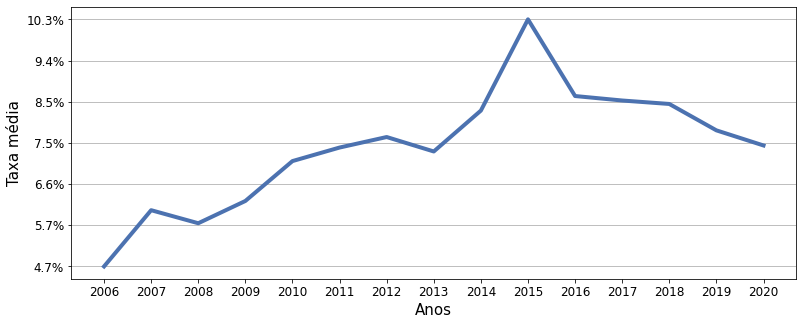
\includegraphics[width=0.8\textwidth]{figuras/taxa_media.png}\\
%	\small \textsuperscript {Fonte: Elaboração própria a partir de dados da Plataforma Atlas do Seguro Rural (Mapa, 2021).}
%   \label{taxa_media}
%\end{figure}

%\begin{small}
%\begin{table}[H]
%\caption{Taxa média de contratação do prêmio de seguro rural por regiões.  Brasil $2006-2020$}\label{tx_media_regioes}
% \input{../anexos/tx_media_regioes.tex}
%\end{table}
%\end{small}

%\subsubsection{Culturas}

A Figura \ref{percent_cult_apol} apresenta o percentual da participação das maiores culturas no número de apólices de seguro rural contratadas. A análise desse gráfico permite identificar que, com exceção de $2015$, a cultura da soja foi a que mais contratou seguro rural. Além disso, observa-se que o milho 2ª safra \footnote{Nesse caso o milho de 2ª safra é listado em separado devido aos distintos graus de risco em relação à 1ª safra \cite{santos17}.} tem cada vez mais aumentado sua participação no número de apólices contratadas. O milho 1ª safra, por sua vez, tem participação que varia entre $1,23\%$ e $16,46\%$, com média de  $6,16\%$ ao longo do período. A participação da cultura da maçã na contratação de seguro rural permanece relativamente estável ao longo do período, variando entre $8,79\%$ e $14,72\%$. 

\begin{figure}[H]
	\centering
	\caption{Percentual da participação das maiores culturas no número de apólices de seguro rural contratadas. Brasil $2006 - 2019$}
    	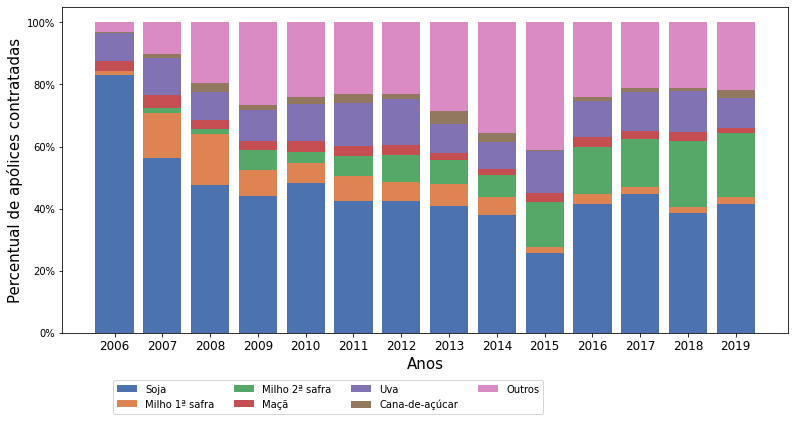
\includegraphics[width=0.8\textwidth]{figuras/percent_apolic_cult.png}\\
	%\small \textsuperscript {Fonte: Elaboração própria a partir de dados do Ministério da Agricultura, Pecuária e Abastecimento \cite{brasil21b}}
	\parbox{\dimexpr\linewidth-2.8cm}{\raggedright
    \strut \textsuperscript{Fonte: Elaboração própria a partir de dados do Ministério da Agricultura, Pecuária e Abastecimento \cite{brasil21b}.}\strut}
    \label{percent_cult_apol}
\end{figure}

A Tabela \ref{percent_culturas} apresenta a participação percentual de grupos de culturas em variáveis do seguro rural. É possível constatar que entre os anos de $2006$ e $2020$, as culturas de grãos foram responsáveis por $74,85\%$ das apólices contratadas, seguida das culturas de frutas com $14,74\%$ das apólices no período. Em terceiro lugar está a cultura de olerícolas, com cerca de $3,36\%$ de participação na contratação de apólices de seguro rural. Uma estrutura semelhante de participação percentual de grupos de culturas pode ser observada com relação à participação no valor total segurado. O grupo de cultura que mais se destaca é a dos grãos, com $74,88\%$ do total segurado, seguido das frutas e do café, com $9,55\%$ e $4,04\%$, respectivamente. 

\begin{small}
\begin{table}[H]
\caption{Participação percentual das culturas nos valores do seguro rural. Brasil $2006-2020$}\label{percent_culturas}
 \footnotesize
\vspace{0.05cm}
\begin{tabularx}{\textwidth}{lRRRRR}
    \hline \\[-1.9ex]	 
    Cultura    & \% das apólices & \% do total segurado & \% do premio total & \% de subvenção & Taxa média \\
    \hline \\[-1.9ex]	 
    Grãos      & 74,85\%         & 74,88\%              & 78,86\%            & 77,35\%         & 7,70\%     \\
    Frutas     & 14,74\%         & 9,55\%               & 13,14\%            & 16,07\%         & 9,17\%     \\
    Olerícolas & 3,36\%          & 2,74\%               & 3,17\%             & 2,85\%          & 7,64\%     \\
    Café       & 3,07\%          & 4,04\%               & 2,19\%             & 1,61\%          & 3,15\%     \\
    Cana       & 2,08\%          & 2,98\%               & 0,77\%             & 0,69\%          & 1,63\%     \\
    Pecuária   & 0,73\%          & 1,16\%               & 0,77\%             & 0,32\%          & 3,26\%     \\
    Floresta   & 0,30\%          & 3,51\%               & 0,42\%             & 0,35\%          & 1,60\%     \\
    Outros     & 0,88\%          & 1,13\%               & 0,68\%             & 0,75\%          & 4,64\%     \\ 
    \hline 
\end{tabularx}
%\vspace{0.5cm}
\small \textsuperscript{Fonte: Elaboração própria a partir de dados da Plataforma Atlas do Seguro Rural (Mapa, 2021).  }\\
\end{table}
\end{small}

Além disso, é possível observar na Tabela \ref{percent_culturas}, os percentuais de subvenção ao prêmio de seguro rural e os valores da taxa média de contratação do seguro. As taxas cobradas durante o período para a cultura de grãos foi de $7,70\%$, a taxa cobrada das culturas de frutas foi de $9,17\%$ e as olerícolas tiveram uma taxa média de contratação de $7,64\%$. Os percentuais de subvenção dessas culturas são, também, os mais altos: $77,35\%$ de subvenção para os grãos, $16,07\%$ para as culturas de frutas e $2,85\%$ para as olerícolas. Ou seja, os grupos de culturas com maior demanda pelo seguro, além de apresentarem os maiores valores de apólices, os maiores valores e maior ocorrência de sinistros, são também aqueles com maiores taxas médias. 

De acordo com  Santos e Silva (2017), este fato pode apontar para a possibilidade de dois fenômenos a serem melhor examinados. O primeiro diz respeito à situação em que as maiores taxas resultam do fato de que maiores subvenções são dadas a cultivos de maior risco. O segundo fenômeno possível é que as taxas sejam mais altas, principalmente no caso dos produtores que adotam o ZARC, com elevada tecnologia produtiva, alta produtividade e não têm estas características levadas em consideração como informação que contribui para a redução das taxas. Dessa forma, se por um lado o seguro agrícola não se consolida sem a subvenção dada pelo Estado, por outro, é possível que esse sistema de subvenção ao prêmio crie distorções no mercado de seguro rural. 

%\subsubsection{Seguradoras}

A Tabela \ref{seguradoras} exibe a distribuição das fatias de mercado das seguradoras entre $2006$ e $2020$. Apesar de as seguradoras passarem de cinco, em $2006$, para $16$ companhias aptas a operar com seguro rural em $2020$, é possível constatar que há uma concentração do mercado de seguro em um número reduzido de seguradoras. 

\begin{small}
\begin{table}[H]
\caption{Participação de mercado das seguradoras. Brasil $2006-2020$}\label{seguradoras}
 \footnotesize
\vspace{0.05cm}
\begin{tabularx}{\textwidth}{lRRRRRRR}
    \hline \\[-1.9ex]	 
    Seguradora         & Apólices        & \% do número de apólices  & Beneficiários  & \% dos beneficiários  & Área segurada (em mil ha)  & \% de área segurada   \\
    \hline \\[-1.9ex]	 
    Brasilseg         &  $410.892$      &  $37,23  $                &  $95.769$                    &  $26,85  $            &  $48.076,26$       & $55,31  $              \\
    Mapfre            &  $149.389$      &  $13,54  $                &  $49.274$                    &  $13,82  $            &  $7.309,17$        &  $8,41  $               \\
    Essor             &  $119.087$      &  $10,79  $                &  $38.995$                    &  $10,93  $            &  $4.603,47$        &  $5,30  $               \\
    Swiss Re          &  $91.410$       &  $8,28  $                 &  $34.483$                    &  $9,67  $             &  $7.870,31$        &  $9,06  $               \\
    Nobre             &  $82.500$       &  $7,48  $                 &  $29.053$                    &  $8,15  $             &  $2.747,88$        &  $3,16  $               \\
    Allianz           &  $66.983$       &  $6,07  $                 &  $21.210$                    &  $5,95  $             &  $5.387,98$        &  $6,20  $               \\
    Sancor            &  $49.567$       &  $4,49  $                 &  $22.516$                    &  $6,31  $             &  $3.210,37$        &  $3,69  $               \\
    Fairfax           &  $35.343$       &  $3,20  $                 &  $18.349$                    &  $5,14  $             &  $2.055,87$        &  $2,37  $               \\
    Porto Seguro      &  $26.306$       &  $2,38  $                 &  $6.152$                     &  $1,72  $             &  $259,33$          &  $0,30  $               \\
    Newe              &  $22.741$       &  $2,06  $                 &  $12.337$                    &  $3,46  $             &  $1.469,10$        &  $1,69  $               \\
    Tokio Marine      &  $19.808$       &  $1,79  $                 &  $11.263$                    &  $3,16  $             &  $1.722,64$        &  $1,98  $               \\
    Too               &  $14.844$       &  $1,35  $                 &  $9.768$                     &  $2,74  $             &  $1.163,48$        &  $1,34  $               \\
    Aliança do Brasil &  $7.200$        &  $0,65  $                 &  $3.294$                     &  $0,92  $             &  $593,19$          &  $0,68  $               \\
    Excelsior         &  $4.472$        &  $0,41  $                 &  $2.292$                     &  $0,64  $             &  $238,97$          &  $0,27  $               \\
    Sompo             &  $3.062$        &  $0,28  $                 &  $1.901$                     &  $0,53  $             &  $181,66$          &  $0,21  $               \\
    Itaú              &  $9$            &  $0,00  $                 &  $9$                         &  $0,00  $             &  $25,10$           &  $0,03  $               \\
    \hline \\[-1.9ex]
    \textbf{Total}    & \textbf{1.103.613} & \textbf{100  }         & \textbf{213.692}             & \textbf{100  }        & \textbf{86.914,79} & \textbf{100  }\\
	\hline 
\end{tabularx}
%\vspace{0.5cm}
\small \textsuperscript{Fonte: Elaboração própria a partir de dados da Plataforma Atlas do Seguro Rural (Mapa, 2021).}\\
\footnotesize{Nota: Valores acumulados $2006 -- 2020$}\\
\end{table}
\end{small}

Ao se analisar a participação no percentual do número de apólices de seguro rural, percebe-se que apenas as três maiores seguradoras (Brasilseg, Mapfre e Essor) concentram cerca de $61,56\%$ do mercado. Com relação ao percentual dos beneficiários, as três maiores seguradoras contam com cerca de $51,60\%$ dos beneficiários durante o período analisado. A concentração é ainda maior quando se analisa o percentual da área segurada, sendo que a  maior seguradora do ramo (Brasilseg) conta com um percentual de $55,31\%$ da área segurada em hectares. As três maiores seguradoras são responsáveis pelo seguro de $72,78\%$ da área segurada. 

%A próxima seção tem como objetivo apresentar os resultados da análise da distribuição espacial dos dados do seguro rural no Brasil. 

\subsection{A DISTRIBUIÇÃO REGIONAL DO SEGURO RURAL} 

Os gráficos apresentados na Figura \ref{variaveis_regioes} exibem a evolução, entre os anos de $2006$ e $2019$, das variáveis de seguro rural analisadas por regiões.

Na figura \ref{ap_contrat_regioes}, é possível observar a evolução do número de apólices contratadas nas regiões brasileiras. Na Figura \ref{ap_contrat_regioes}, observa-se que a região Sul se destaca das demais com relação ao número de apólices contratadas. O menor número de apólices contratadas na região Sul foi de $16.525$ apólices no ano de $2006$. O valor médio de apólices contratadas durante o período foi $44.166$ apólice. No ano de $2014$, foi registrado o maior número de apólices contratadas ($76.668$ apólices). 

% variaveis_regioes
\begin{figure}[H]
	\centering
	\caption{Evolução das variáveis de seguro rural por regiões. Brasil $2006 - 2019$}\label{variaveis_regioes}
	\small
	
	\subfloat[Número de apólices contratadas\label{ap_contrat_regioes}]{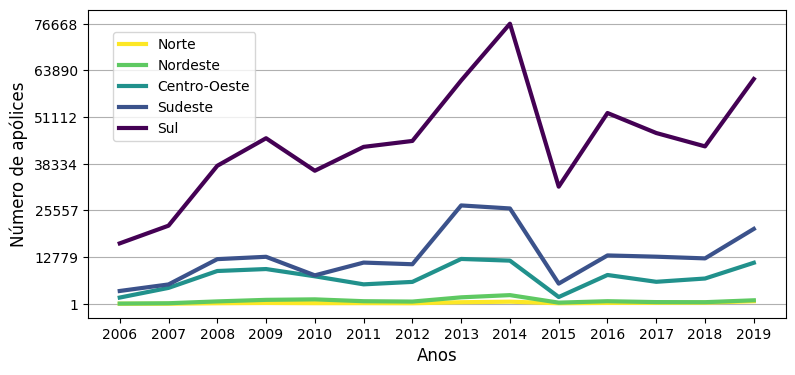
\includegraphics[width=0.45\textwidth]{figuras/ap_contrat_regioes.png}}\hspace{0.1cm}
	\subfloat[Total segurado (em milhões de R\$)\label{t_segurado_regioes}]{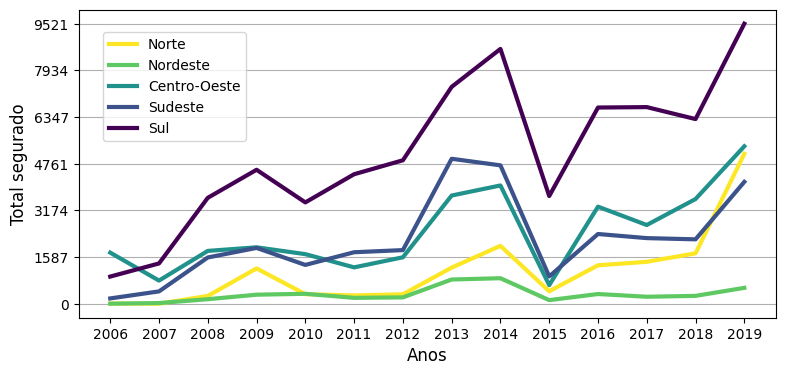
\includegraphics[width=0.45\textwidth]{figuras/t_segurado_regioes.png}}\\
	
	\subfloat[Valores de prêmio (em milhões de R\$)\label{soma_premio_regioes}]{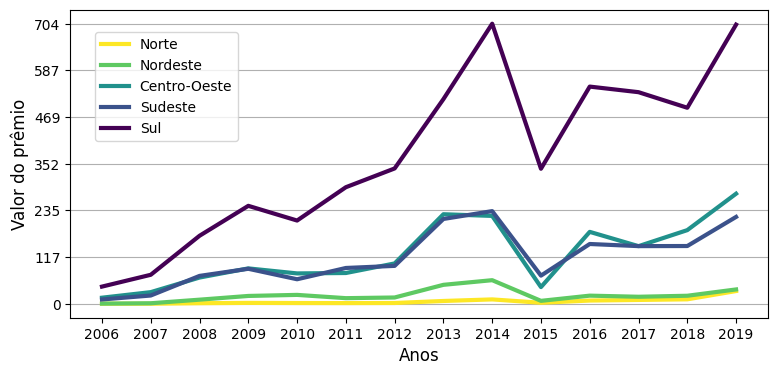
\includegraphics[width=0.45\textwidth]{figuras/soma_premio_regioes.png}}\hspace{0.1cm}
	\subfloat[Valores subvenção (em milhões de R\$)\label{t_subvencao_regioes}]{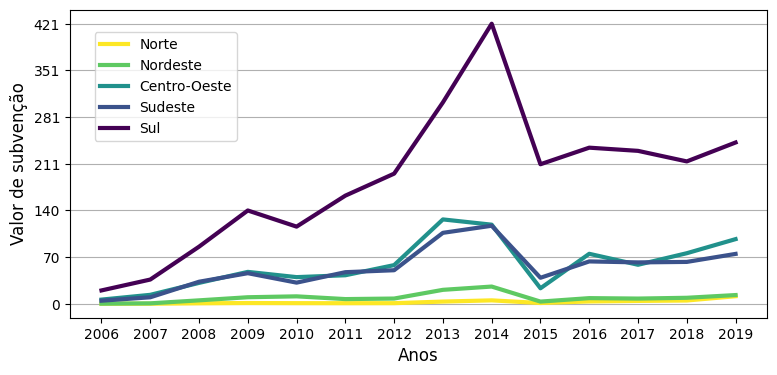
\includegraphics[width=0.45\textwidth]{figuras/t_subvencao_regioes.png}}\\
	
	\subfloat[Apólices indenizadas\label{ap_indeniz_regioes}]{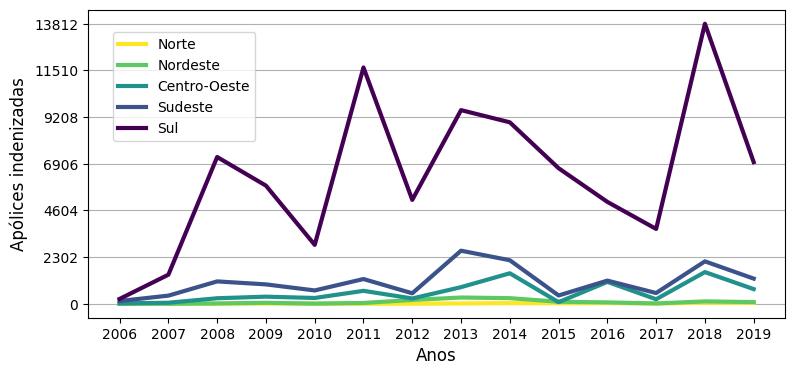
\includegraphics[width=0.45\textwidth]{figuras/ap_indeniz_regioes.png}}\hspace{0.1cm}
	\subfloat[Valor das indenizações (em milhões de R\$)\label{inde_pagas_regioes}]{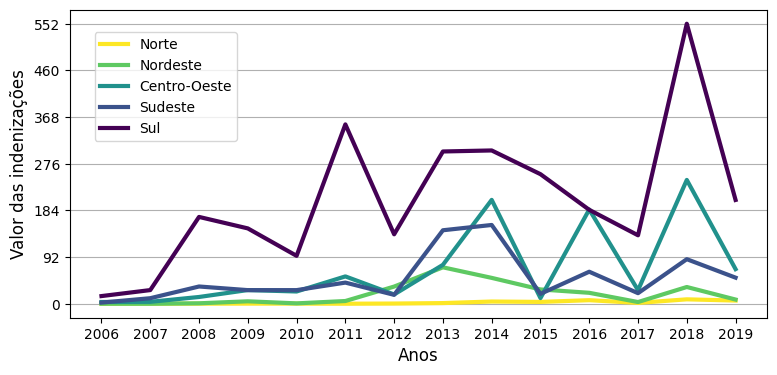
\includegraphics[width=0.45\textwidth]{figuras/inde_pagas_regioes.png}}\\
	
    \parbox{\dimexpr\linewidth-2cm}{\raggedright
    \strut \textsuperscript{Fonte: Elaboração própria a partir de dados do Ministério da Agricultura, Pecuária e Abastecimento \cite{brasil21b}}\strut}
\end{figure}

A segunda região com maior número de apólices contratadas é a região Sudeste (Figura \ref{ap_contrat_regioes}). Em média, na região Sudeste, foram contratadas $12.942$ apólices por ano, o maior valor registrado foi $26.913$ apólices contratadas em $2013$. A região Centro-Oeste é a terceira região com mais apólices contratadas, sendo que em média foram contratadas $7.225$  por ano e, em $2013$ foi registrado o maior número de apólices ($12.260$). Por fim, as regiões Norte e Nordeste, apresentaram respectivamente, em média, $240$ e $804$ apólices contratadas por ano.

A taxa de crescimento do número de apólices contratadas na região sul foi de $3,72$ vezes o valor inicial entre os anos $2006$ e $2019$. Por sua vez, durante o período analisado a região Sudeste teve um crescimento do número apólices de $5,87$ vezes e a região Centro-Oeste apresentou um crescimento do número de apólices de $6,66$ vezes. As regiões Norte e Nordeste apresentaram um crescimento médio anual igual a $0,14\%$ e $4,04\%$ respectivamente. 

Ao se analisar a evolução do total segurado nas regiões brasileiras apresentado na Figura \ref{t_segurado_regioes}, é possível observar que a região Sul se destaca com, em média, $5146,83$ milhões de valor segurado total. O maior valor foi registrado em $2019$ e foi igual a $9520,85$ milhões, o segundo maior valor foi igual a $8664,31$ milhões e foi registrado em $2015$. 

No início da série valores a região Centro-Oeste apresenta um maior valor total segurado do que a região Sul (5.355 milhões). Além disso, como é possível observar na Figura \ref{t_segurado_regioes}, a partir do ano de $2016$ a região Centro-Oeste supera a região Sudeste no valor total segurado. A região Norte apresentou, com relação ao total segurado, os valores de $120,35$ milhões em $2009$ e $197,01$ milhões em $2014$. 
Além disso, a região Norte apresenta o seu maior valor no ano de $2019$, com total segurado igual a $509,94$ milhões. Também é possível observar que há indícios de haver um crescimento do total segurado em todas as regiões. 

O total segurado na região Sul apresenta um crescimento de cerca de $10,27$ vezes entre os anos de $2006$ e $2019$. Na região Sudeste, o crescimento foi de $22,52$ vezes o valor registrado em $2006$. Por sua vez, o Centro-Oeste apresentou um crescimento de cerca de $3,07$ vezes o valor do total segurado durante o período. O valor do total segurado na região Norte cresceu $499.51$ vezes entre os anos $2006$ e $2019$. Por fim, no Nordeste, o valor total segurado apresentou um crescimento de $106,95$ vezes o valor inicial. 

Para mais, ao se analisar a Figura \ref{soma_premio_regioes} e \ref{t_subvencao_regioes}, é possível observar que as variáveis valores de prêmio e valores subvenção apresentam crescimento durante o período analisado. Também é possível observar que, com exceção das variáveis relacionadas à indenização, as variáveis apresentam uma queda entre os anos de $2014$ e $2015$.

É possível observar na Figura \ref{ap_indeniz_regioes}, que a região Sul se destaca quando se analisa o número de apólices indenizadas. Os valores variam de $237$ em $2006$ e $13812$ apólices indenizadas em $2019$. Em média, a região Sul teve cerca de $6364$ apólices indenizadas durante o período. Além disso, durante os anos analisados, houve um crescimento de $58,28\%$ no número de apólices de seguro rural indenizadas. A região Sudeste é a segunda região com maior número de apólices indenizadas, sendo que o menor número de apólices indenizadas na região Sudeste foi de $135$ e ocorreu em $2006$, com maior valor registrado em $2013$, equivalente a $2.616$. 

Ao longo dos anos analisados, a diferença entre o número de apólices na região Sul e Sudeste foi em média igual a $5.283$ apólices. A região Centro-Oeste foi responsável por, em média, $559,64$ apólices indenizadas. O maior número de apólices indenizadas na região Centro-Oeste foi registrado em $2018$ e foi igual a $1561$ apólices. As regiões Norte e Nordeste tiveram em média $15,57$ e $88,64$, respectivamente. 

Com relação ao valor das indenizações de seguro rural pagas, é possível observar na Figura \ref{inde_pagas_regioes}, que a região Sul é a que possui os maiores valores pagos como indenização. Em média, foram pagos R$\$205,66$ milhões como indenização. O maior valor foi equivalente a R$\$551,74$ milhões e foi registrado em $2018$ e o menor valor foi registrado no primeiro ano analisado, sendo equivalente a R$\$15.06$ milhões. 

A Tabela \ref{media_regioes} apresenta a média dos valores anuais das variáveis de seguro rural acumulados por regiões no Brasil no período de $2006$ e $2019$. Como é possível observar, que a região Sul se destaca das demais com os maiores valores das médias das variáveis. Com relação ao número de apólices contratadas, a segunda região com maior média da variável total de apólices contratadas é o Sudeste. No entanto, quando se analisa a média da soma da importância seguradas, a segunda região com maior média é a região Centro-Oeste. A região Centro-Oeste, também conta com maiores médias nas variáveis soma dos prêmios pagos, total da subvenção e soma das indenizações pagas com relação às regiões Norte, Nordeste e Sudeste. A região Sudeste apresenta a maior média anual do número de apólices indenizadas. 



\begin{small}
\begin{table}[H]
\caption{Média anual dos valores das variáveis de seguro rural por regiões. Brasil $2006-2019$}\label{media_regioes}
\begin{center}
\footnotesize
    \begin{tabular}{lrrrrr}
    \hline \\[-1.9ex]	
    Variável                                  & Norte   & Nordeste & Centro-Oeste & Sudeste  & Sul       \\
    \hline \\[-1.9ex]	
    Total de apólices contratada              &  240,14 &   803,57 &      7.225,36 &  12.941,5 &  44.166,14 \\
    Soma da importância segurada (R\$ milhão) &   111,5 &   319,82 &      2.428,79 &  2.178,54 &   5.146,84 \\
    Soma dos prêmios (R\$ milhão)             &    6,37 &    20,76 &       123,43 &   115,02 &    371,72 \\
    Total de subvenção (R\$ milhão)           &    2,66 &     9,25 &        58,25 &    53,52 &    186,56 \\
    Soma das indenizações pagas (R\$ milhão)  &    2,39 &    18,73 &        68,59 &    50,15 &    205,66 \\
    Taxa média aplicada às apólices           &    0,01 &     0,01 &         0,13 &     0,11 &      0,45 \\
    Número de apólices indenizadas            &   15,57 &    88,64 &       559,64 &  1.081,57 &   6.364,57 \\
    \hline 
    \end{tabular}
\end{center}
\small \textsuperscript {Fonte: Elaboração própria a partir de dados do Ministério da Agricultura, Pecuária e Abastecimento (MAPA)}\\


\end{table}
\end{small}

A média dos valores anuais da taxa média de contratação de apólices indica que, a região Sul é a que possui maior taxa de contratação de seguro com taxa média igual a $0,45$ ao longo dos anos. A região Centro-Oeste é a que tem o segundo maior valor de taxa média durante os anos, sendo igual a $0,13$. As regiões Norte e Nordeste apresentaram taxa média igual a $0,01$.

\subsection{DISTRIBUIÇÃO ESPACIAL DO SEGURO RURAL}

A análise da distribuição espacial das variáveis se inicia com a visualização dos mapas temáticos. Por meio destes mapas, busca-se identificar visualmente se há a ocorrência de padrões na distribuição espacial das variáveis do seguro rural.

O primeiro grupo de mapas, apresentado na Figura \ref{map_segurado}, exibe a distribuição espacial da soma da importância segurada (R\$ milhão) nos municípios brasileiros entre os anos de $2006$ e $2019$. Para a construção dos mapas, os valores da variável foram divididos em 5 intervalos \footnote{Para a criação dos intervalos foi aplicado algoritmo Fisher Jenks aos valores das variáveis diferentes de $0$ e os intervalos foram criados tendo como referência os valores do ano de 2019 \cite{jenks77}}.

\begin{figure}[H]
	\centering
	\caption{Total segurado por municípios (em mil R\$). Brasil $2006 - 2019$}
	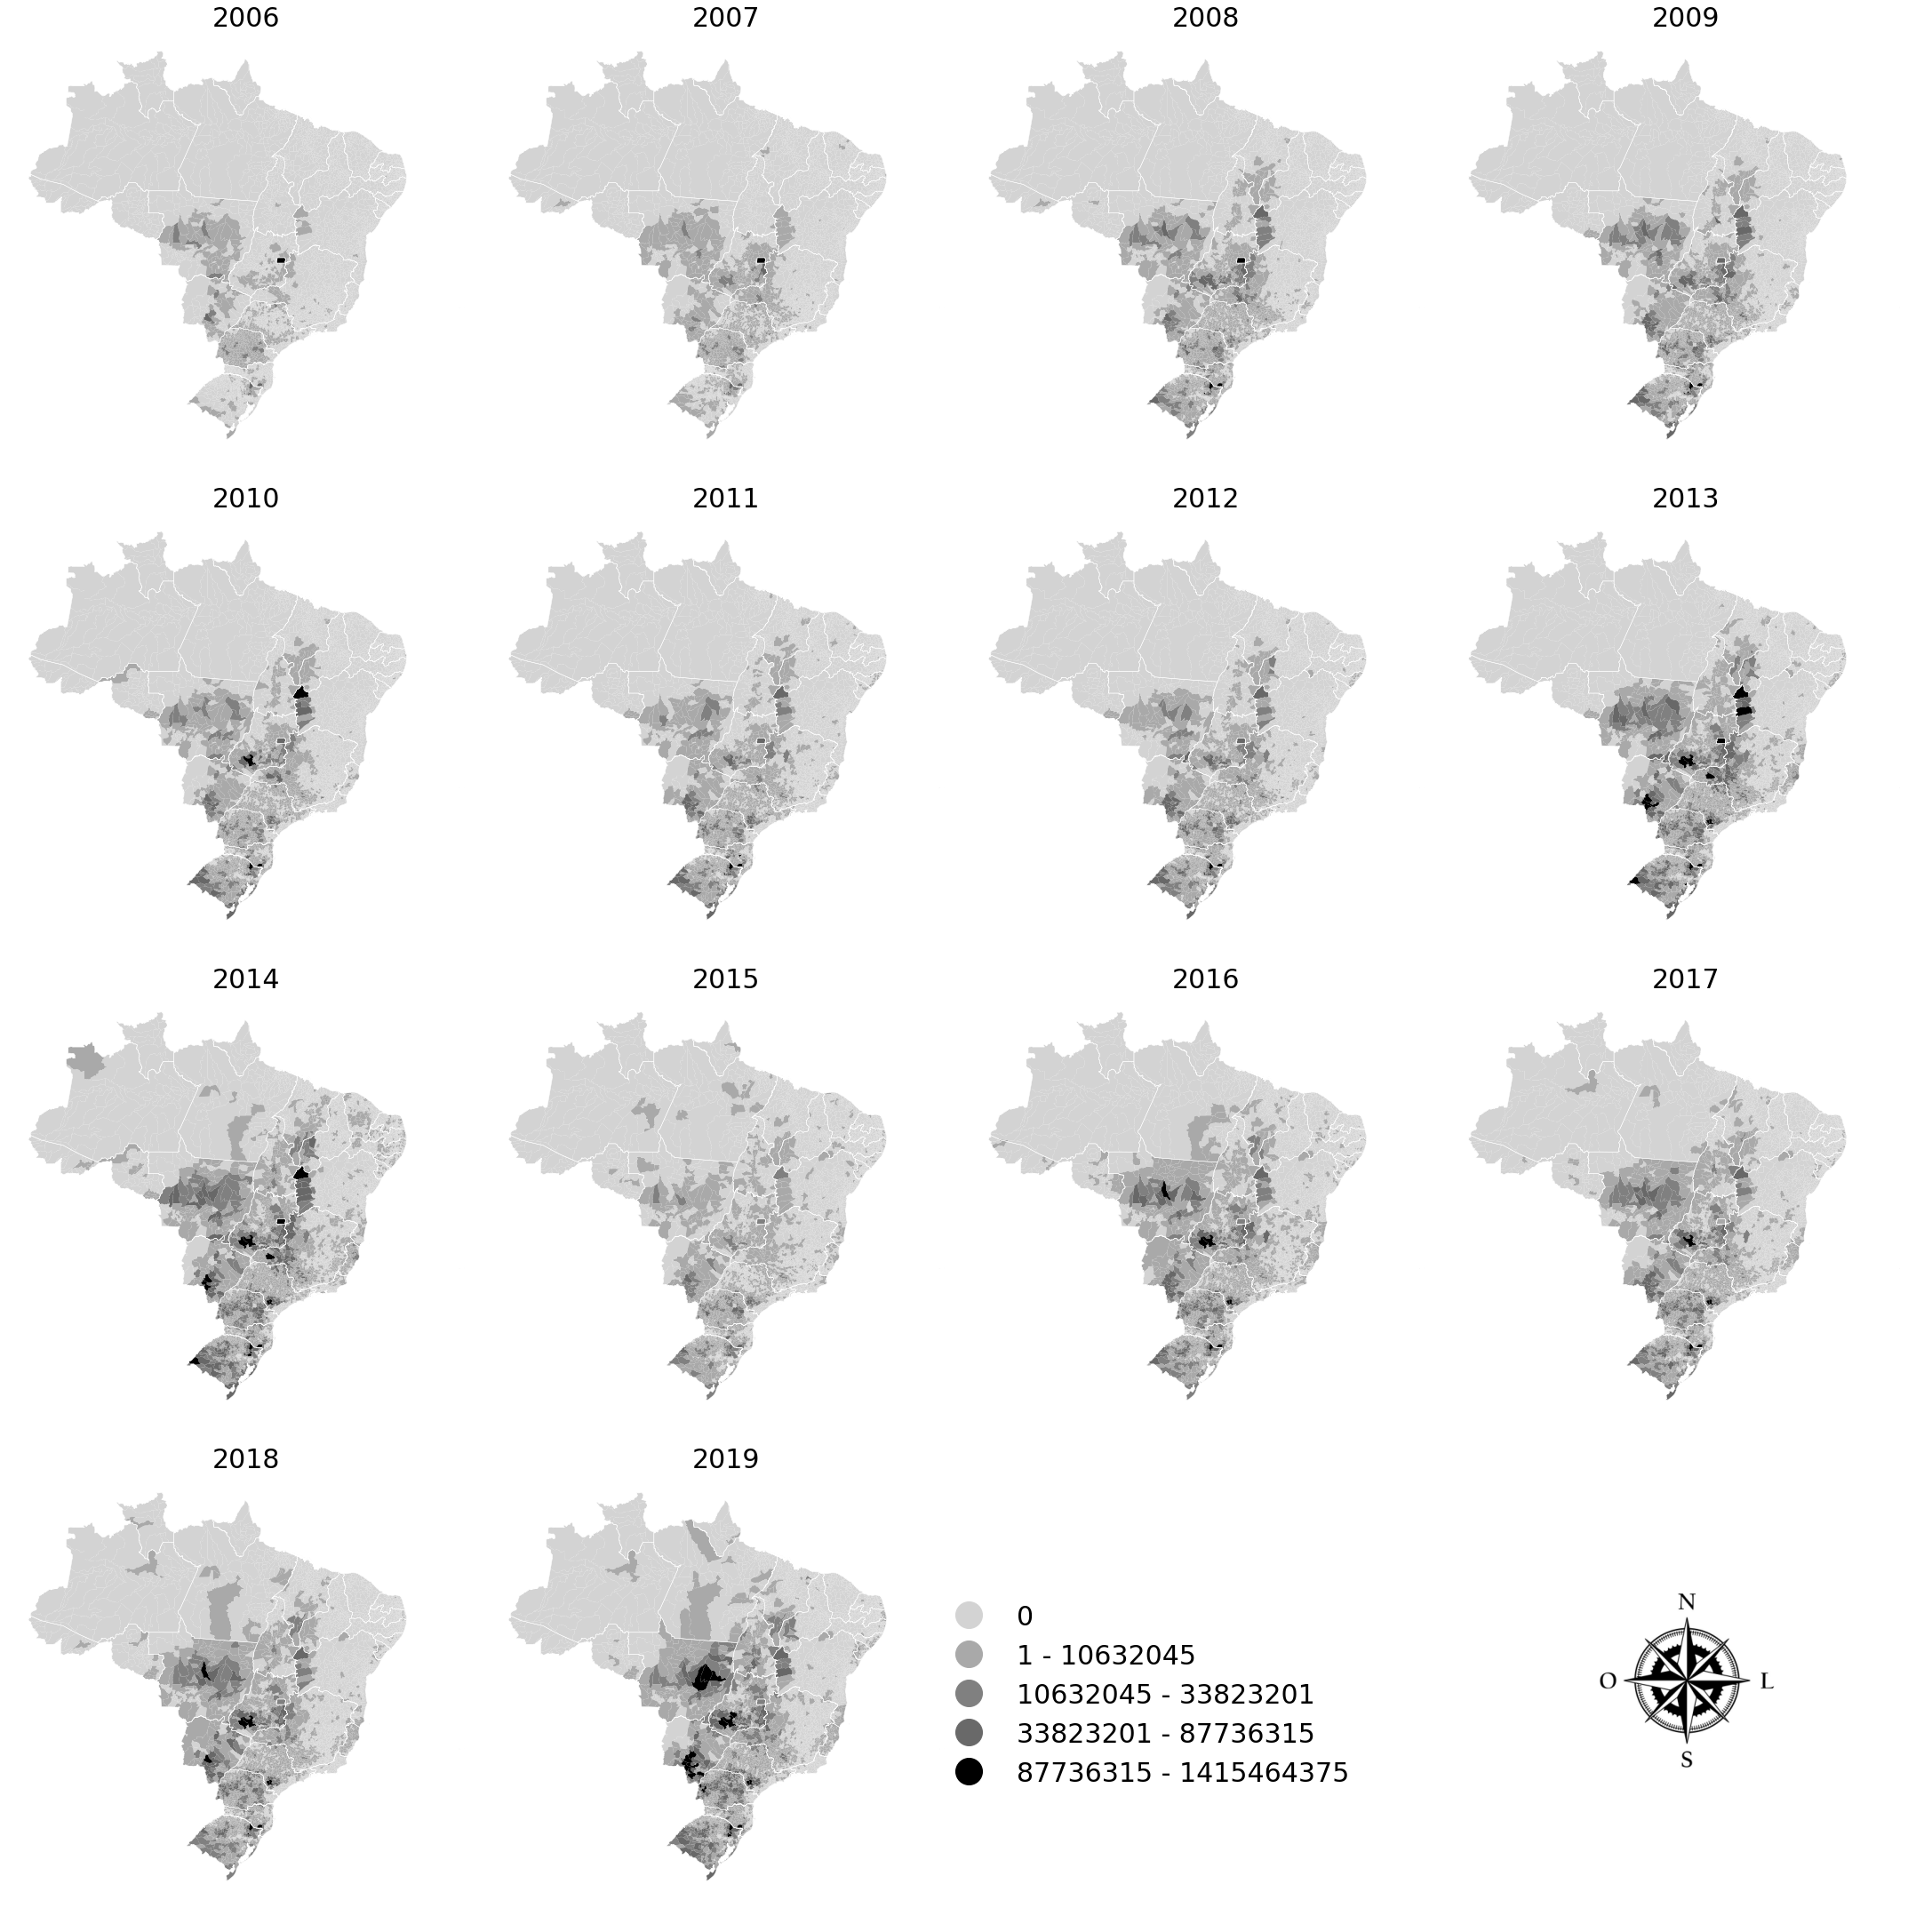
\includegraphics[width=0.9\textwidth]{figuras/map_total_segurado_mil.png}
	\small \textsuperscript {Fonte: Elaboração própria a partir de dados do Ministério da Agricultura, Pecuária e Abastecimento \cite{brasil21b}}
    \label{map_segurado}
\end{figure}

Pela análise da Figura \ref{map_segurado}, é possível observar que a distribuição espacial do total segurado se modificou no decorrer dos anos, apesar de se concentrar principalmente nas Regiões Sul e Centro-Oeste. É possível também destacar que, durante o período analisado, há indícios de concentrações espaciais na região do Extremo Oeste Baiano no Estado da Bahia, Sudoeste de Mato Grosso do Sul, Sul Goiano no Estado de Goiás e Sudeste, no sul do Estado de São Paulo.

O conjunto de mapas apresentado na Figura \ref{map_apolices}, exibe o número de apólices de seguro rural contratadas por municípios entre $2006$ e $2019$. Ao longo dos anos, o número de municípios com nenhuma apólice contratada cai e há indícios de um aumento do número de apólices até o ano de $2014$. Entre os anos de $2014$ e $2015$, há uma queda no número de apólices contratadas, como já foi mostrado no gráfico da Figura \ref{apolices_produtores}, e das demais variáveis relacionadas ao seguro rural. Essa redução também pode ser visualizada no mapa da Figura \ref{map_apolices}, em que o ano de $2015$ apresenta municípios com menor número de apólices contratadas. 

Ao se analisar a distribuição espacial, observa-se que há indícios de haver uma maior concentração espacial do total segurado e do número de apólices de seguro rural contratadas em algumas regiões. A partir do ano de $2015$ a retomada do crescimento destas variáveis (Figura \ref{total_segurado_mil}) pode ser visualizado com um maior número de áreas de coloração mais escura nos mapas (Figuras \ref{map_segurado} e \ref{map_apolices}).

\begin{figure}[H]
	\centering
	\caption{Número de apólices de seguro rural contratadas por municípios. Brasil $2006 - 2019$}
	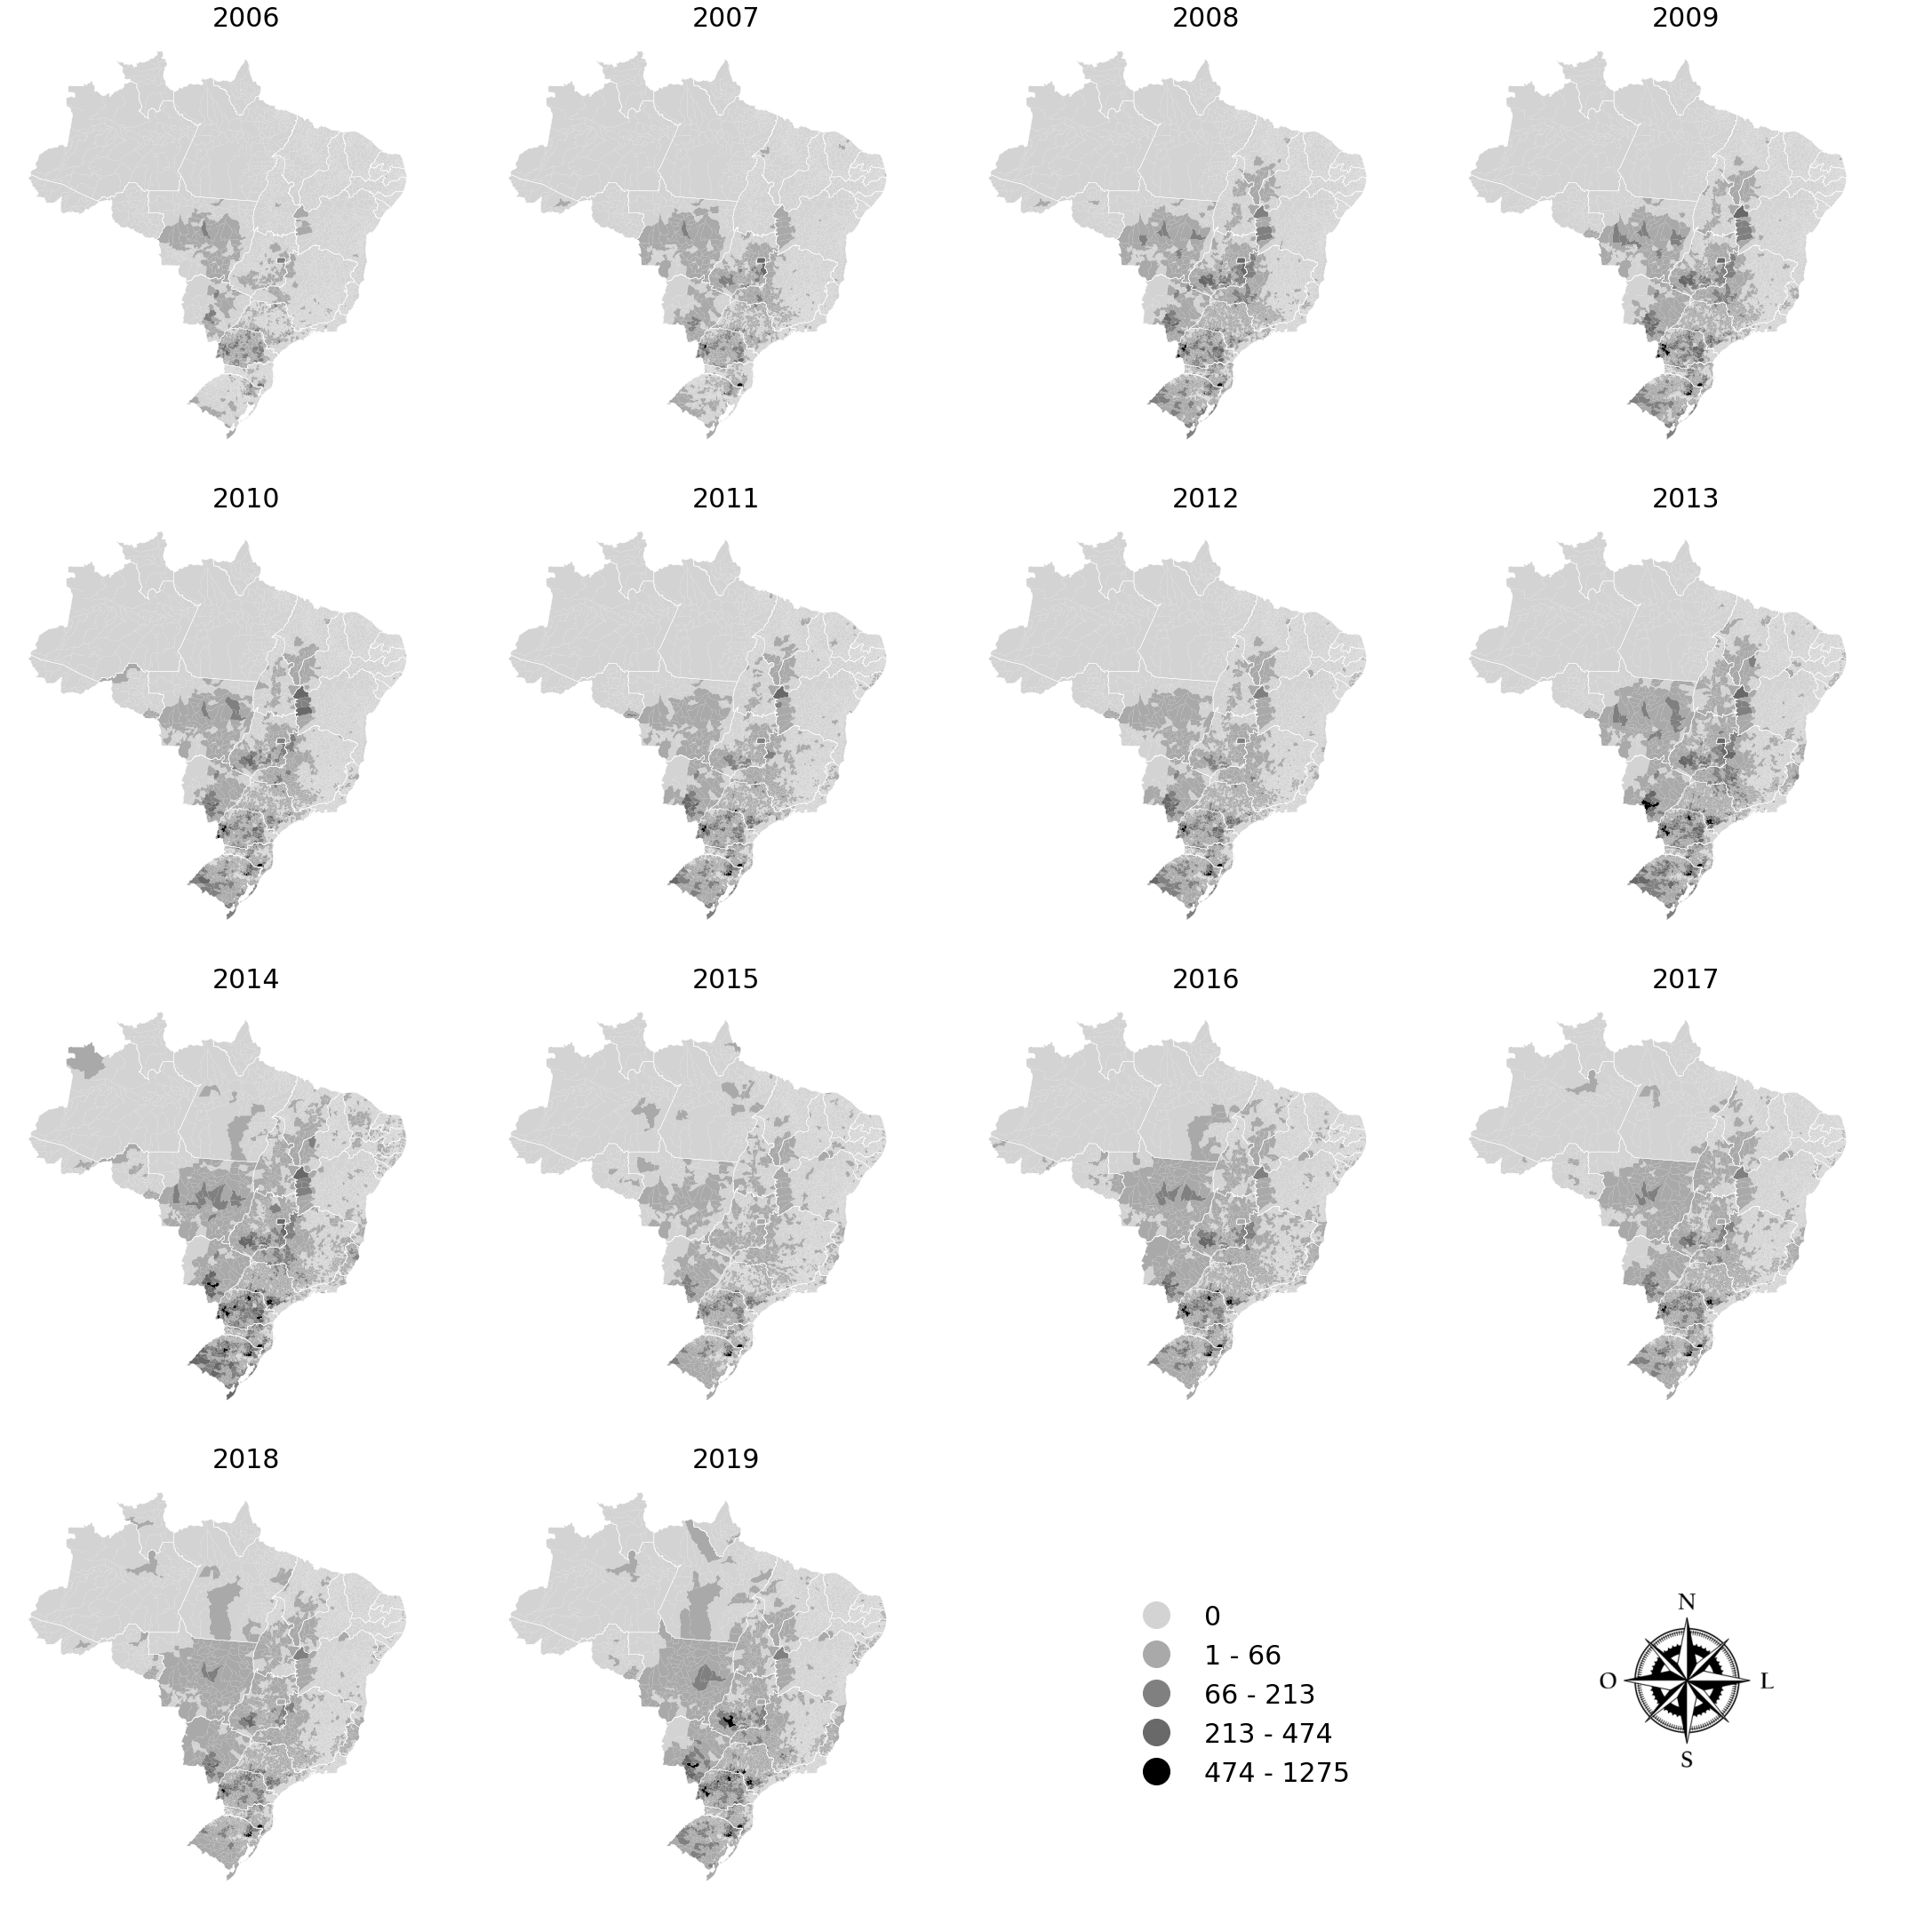
\includegraphics[width=0.9\textwidth]{figuras/map_apolices_contratadas.png}
	\small \textsuperscript {Fonte: Elaboração própria a partir de dados do Ministério da Agricultura, Pecuária e Abastecimento \cite{brasil21b}}
    \label{map_apolices}
\end{figure}

A distribuição espacial das demais variáveis analisadas apresenta um padrão semelhante ao observado com a soma da importância segurada (R\$ milhão)  \footnote{Os mapas da distribuição espacial das variáveis do seguro rural no Brasil são apresentados no apêndice A}. Dessa forma, os resultados corroboram a hipótese apresentada por Silva, Teixeira e Santos (2014) na investigação sobre a participação do PSR na universalização do acesso ao seguro rural. Ou seja, apesar da evolução do seguro rural em âmbito nacional, quando se observa a distribuição espacial, verifica-se que há, ao longo do tempo, uma concentração das apólices e subvenções na região Sul e Centro-Oeste. Portanto, apesar de ter ocorrido uma ampliação do seguro rural, esta ampliação ocorreu de forma concentrada, o que evidencia o cumprimento de forma parcial dos objetivos do PSR \cite{silva14}.

\section{CONSIDERAÇÕES FINAIS}

%O objetivo do presente trabalho foi analisar a evolução e a dinâmica espacial de variáveis do seguro rural nos municípios brasileiros entre 2006 e 2019. Além disso, buscou-se investigar a presença de padrões de distribuição espacial. A

A análise possibilitou constatar resultados positivos na evolução do seguro rural no Brasil. O número de apólices contratadas tem um crescimento de cerca de $8,69$ vezes seu valor inicial durante o período. Ademais, a área agrícola segurada no país praticamente dobrou entre os anos de $2019$ e $2020$, quando alcançou o maior valor, $13,7$ milhões de hectares, que representa $20\%$ da área total agrícola do país. 

Em geral, identificou-se que as maiores concentrações de apólices de seguro rural estão situadas nas regiões Sul, Centro-Oeste e Sudeste, no sul do Estado de São Paulo.  Para mais, ressalta-se que, embora mantenham a concentração do número de apólices contratadas, número de apólices indenizadas, valores de subvenção, indenização e prêmio, atualmente há expansão da demanda por seguros agrícolas. 

Apesar de os dados indicarem uma concentração geográfica da adesão ao sistema de seguro rural no Brasil, é necessário levar em consideração outros sistemas, como o Proagro e o programa Garantia Safra. É necessário, ainda, ressaltar que a adesão dos produtores deve ocorrer como uma resposta à percepção do risco das atividades agropecuárias, ou seja, o seguro deve difundir-se com base na compreensão dos riscos e das vantagens de sua contratação. 

Por fim, este trabalho pode ser entendido como uma abordagem inicial, a partir da qual é possível se introduzir novos métodos estatísticos a fim de aprimorar os resultados. Dentre esses métodos, destaca-se a Análise de Componentes Principais (ACP), que pode ser utilizada para reduzir o número de variáveis,  de forma a possibilitar a incorporação de informação de mais de uma variável na análise exploratória espacial.

\newpage
\addcontentsline{toc}{section}{\hspace*{\distnumber}REFERÊNCIAS}
\begin{center}
\section*{REFERÊNCIAS} 
\end{center}




% Use isso descomentado durante edição.
% Quando concluir a Tese, comente isso e use
% o código do bloco abaixo.
%\begin{singlespace}
%\renewcommand\refname{}
%\begin{flushleft}
%\bibliography{../tese/bibtese2}
%\end{flushleft}
%\end{singlespace}

%% Em cap1intriduc-corrigido.bbl foi feita correção manual de
%% algumas referências como por exemplo as citações
%% de Dissertação e Tese.
%% Então deixa-se de usar o arquivo cap1introduc.bbl gerado
%% automaticamente pelo abntcite, mas isso é só ao final.
\begin{singlespace}
\begin{flushleft}
\renewcommand\refname{}
\vspace*{-1.5cm}
\documentclass[10pt]{article}
%==========================================================================================

\usepackage[utf8]{inputenc}
\usepackage[brazil]{babel}
\usepackage[T1]{fontenc}
\usepackage{amsmath}
\usepackage{amsfonts}
\usepackage{mathrsfs}
\usepackage{amssymb}
\usepackage{graphicx}
\usepackage{geometry, calc, color, setspace}
\usepackage{indentfirst}
\usepackage{wrapfig}
\usepackage{boxedminipage}
\usepackage{enumerate}
\usepackage{float}
\usepackage{paralist}
\usepackage{comment}
\usepackage{icomma}
\usepackage{rotating}
\usepackage{multirow}
\usepackage[position=bottom]{subfig}
\usepackage{array}
\usepackage{tabularx}
\usepackage{float}
\usepackage{array}

\newcolumntype{L}[1]{>{\raggedright\let\newline\\\arraybackslash\hspace{0pt}}m{#1}}
\newcolumntype{C}[1]{>{\centering\let\newline\\\arraybackslash\hspace{0pt}}m{#1}}
%\newcolumntype{R}[1]{>{\raggedleft\let\newline\\\arraybackslash\hspace{0pt}}m{#1}}
\newcolumntype{R}{>{\raggedleft\let\newline\\\arraybackslash\hspace{0pt}}X}

\usepackage[alf,bibjustif]{abntex2cite}
%\usepackage{abntcite}

% Para o alinhamento dos títulos das figuras
\usepackage{caption}
%\captionsetup[figure]{format=hang,labelsep=endash,font=small,justification=RaggedRight,singlelinecheck=off, margin=1cm}
\captionsetup[subfigure]{textfont=small,singlelinecheck=off,justification=raggedright}


%%  Inserindo os códigos Python ==================================
\usepackage{listings}

%\definecolor{light_gray}{rgb}{0.97,0.97,0.97}
%\definecolor{mymauve}{rgb}{0.58,0,0.82}
%\definecolor{mygreen}{rgb}{0,0.6,0}

\lstset{
  language = Python,
  inputencoding = utf8,
  backgroundcolor = \color{white},
  columns=fullflexible,
  basicstyle=\ttfamily,
  breaklines=true,
  postbreak=\raisebox{0ex}[0ex][0ex]{\color{black}$\hookrightarrow$\space},
  keywordstyle=\color{black},      % keyword style
  stringstyle=\color{black},
  commentstyle=\color{black}
}

\newcommand{\HRule}{\noindent\rule{\linewidth}{0.2mm}}

\usepackage{mathpazo}                         % tem suporte matemático
\usepackage[scaled=0.85]{beramono}            % usa esta nos verbatins [scaled=0.9]

\renewcommand\UrlFont{\color{black}\rmfamily} 

\def\distnumber{2.3em}

%==========================================================================================

\author{Walef Machado de Mendonça\footnote{Mestrando em Estatística Aplicada e Biometria na Universidade Federal de Alfenas}\\
Patrícia de Siqueira Ramos\footnote{Professora da Universidade Federal de Alfenas, campus Varginha}}

%==========================================================================================


\title{O seguro rural no Brasil: evolução e distribuição espacial}

\date{}

\begin{document}

\maketitle

\begin{abstract}
As atividades agropecuárias se inserem em um contexto de adversidades que as colocam em situação diferenciada em relação aos riscos enfrentados pelos produtores. Tais atividades demandam grandes investimentos, o que faz com que sua atratividade esteja relacionada às formas existentes de gerenciamento de riscos. Uma das formas mais usuais de gerenciamento de risco neste setor é a contratação de Seguro Rural, uma vez que esta modalidade de seguro possibilita a recuperação da capacidade financeira do produtor na ocorrência de sinistros. Nesse sentido, o objetivo do trabalho é avaliar a distribuição e a dinâmica espacial de variáveis relacionadas às apólices de Seguro Rural contratadas nos municípios brasileiros no período de 2006 a 2019. Além disso, busca-se investigar a existência de dependência espacial e a presença de agrupamentos com grande número de apólices de Seguro Rural. Para tanto, utiliza-se os dados dos Censos do Seguro Rural, compilados pelo Ministério da Agricultura, Pecuária e Abastecimento (MAPA) e Análise Exploratória de Dados Espaciais (AEDE). Os resultados apontam que as maiores concentrações de apólices de Seguro Rural estão situadas nas regiões Sul e Centro-Oeste. Além disso, apesar de haver um aumento nas contratações de Seguro Rural, há também uma tendência de maior concentração espacial das apólices ao longo do período analisado. \\
\newline
\noindent {\textbf{Palavras-chave}}: Seguro rural. Política agrícola. Estatística espacial. Autocorrelação espacial. I de Moran.
\end{abstract}

\section{INTRODUÇÃO}

O setor agropecuário brasileiro tem se destacado nas últimas décadas por seu crescimento proveniente da aplicação de novas tecnologias ao clima tropical e a incorporação de novas áreas de terras \cite{brasil19a}. Segundo dados dos censos agropecuários, entre $2006$ e $2017$, tanto a área total quanto a produção agrícola e pecuária vivenciaram crescimento. Neste período houve um acréscimo de cerca de $5,8\%$ na área total dos estabelecimentos agropecuários \cite{ibge19}. Com relação à sua participação no PIB, em 2019, a parcela do agronegócio brasileiro foi de  $20,5\%$  do PIB nacional. Já em 2020, o setor agropecuário brasileiro alcançou a participação de $26,6\%$ do PIB. Em valores monetários, o PIB do País totalizou R\$ $7,45$ trilhões em 2020, e a participação do agronegócio chegou a quase R\$ $2$ trilhões \cite{cepea21}. 

Dada a relevância do setor agropecuário na economia brasileira, é necessário destacar que este ramo apresenta características muito específicas com relação à magnitude dos riscos aos quais está sujeito \cite{burgo05}. Alguns riscos mais relevantes se devem, principalmente, às instabilidades climáticas e ameaças sanitárias, que podem afetar a produção, ou à razões de mercado, como variações das taxas de câmbio e juros, ou a condições ligadas ao ambiente de negócios, tais como, alterações em marcos regulatórios e em políticas públicas. Todos esses fatores geram variações na renda do setor, que devem ser enfrentadas por meio de políticas de apoio à gestão de riscos \cite{brasil21}. 

Uma gestão de riscos apropriada tem potencial de afetar de forma positiva a estabilidade da renda do produtor e sua própria permanência no setor agropecuário. O gerenciamento de riscos agropecuários pode ocorrer de diversas maneiras, no entanto, a contratação de seguro é uma das medidas mais comuns. O seguro rural é uma importante ferramenta de mitigação de riscos e proteção da renda. Esta modalidade de seguro atua no sentido de amenizar as perdas e possibilitar a recuperação da capacidade financeira do produtor rural em caso de ocorrência de sinistros \cite{brasil19b}. 

Nesse sentido, o presente trabalho tem por objetivo, avaliar a distribuição espacial do seguro rural nos municípios brasileiros entre 2006 e 2019. Para tanto, busca-se investigar se, no Brasil, as variáveis de seguro rural se distribuem de forma aleatória no espaço ou se há padrões de distribuição espacial. Além disso, através da análise da distribuição espacial do seguro rural no período, busca-se identificar se há regiões que tiveram alterações significativas no número de contratações de seguro. Por fim, este estudo busca fornecer informações para o debate de aperfeiçoamentos no sistema de seguro rural brasileiro, de forma a contribuir para uma agricultura mais eficiente e com menores riscos para o produtor rural.

O trabalho está estruturado da seguinte forma: a próxima seção apresenta uma breve revisão de literatura sobre o seguro rural. A terceira seção apresenta os dados, os procedimentos de análise e recursos computacionais que serão utilizados. A quarta seção apresenta resultados e discussões. A última seção apresenta as considerações finais.

\section{UM PANORAMA DO SEGURO RURAL NO BRASIL}

No Brasil, as primeiras iniciativas de se instalar um sistema de seguro rural remontam à meados da década de $1930$ e desenvolveram-se principalmente nas esferas estaduais. Em $1939$, o Estado de São Paulo determinou a criação de um seguro obrigatório contra o granizo na produção de algodão \cite{maia11}. Segundo Silva, Teixeira e Santos (2014), os resultados do seguro para a proteção da lavoura algodoeira em São Paulo influenciaram a criação de novos programas como a Carteira de Seguro Agrícola contra Granizo para a Viticultura, criada em $1948$, e a Carteira de Seguro Agrícola contra Geada para Horticultura instituída em $1964$.

Além disso, Silva, Teixeira e Santos (2014) apontam em seu trabalho o seguro para granizo que foi criado no final da década de $1940$ no Instituto Rio-Grandense do Arroz (Irga), e o seguro criado pela Associação dos Fumicultores do Brasil (Afubra), que objetivava ressarcir com recursos próprios os produtores de fumo nos estados de Santa Catarina e Rio Grande do Sul.

Já no âmbito nacional, foi criado em $1948$, o Instituto de  Resseguros do Brasil (IRB), com o objetivo de reduzir os prejuízos de eventos adversos e assegurar uma maior estabilidade aos produtores rurais \cite{silva14}. Além disso, o Governo Federal criou, em $1954$, a Companhia Nacional de Seguro Agrícola (CNSA) e o Fundo de Estabilidade do Seguro Agrário. Para mais, Maia,  Roitman e de Conti (2011) evidenciaram que a estruturação e gestão dos seguros da CNSA ficaram, de início, sob responsabilidade do IRB. No entanto, segundo Gemignani (2000), as atividades da CNSA se encerraram em $1996$, em decorrência do insucesso em disseminar a adesão ao seguro rural de forma a possibilitar sua viabilidade econômica \cite{maia11, silva14}.

Na segunda metade da década de $1960$, são instituídos o Decreto-Lei nº $73$ ($1966$) e o Decreto nº $60.459$ ($1967$), que instituem os fundamentos institucionais para as atividades de seguro e a criação do Sistema Nacional de Seguros Privados (SNSP). O decreto de $1967$ também criou o Fundo de Estabilidade do Seguro Rural (FESR), cujos recursos inicialmente eram geridos pelo IRB e cujo objetivo principal era garantir a equilíbrio do sistema de seguro rural e fornecer uma cobertura adicional para os riscos de sinistro \cite{silva14}

% Até aqui Ok
Instituída em $1970$, a Resolução nº $5$ do Conselho Nacional de Seguros Privados teve uma função relevante na caracterização das modalidades de seguros agrários. Nesta Resolução, foi definido o seguro agrícola, que fornece cobertura contra perdas decorrentes de fenômenos meteorológicos, doenças e pragas, o seguro pecuário que fornece cobertura para morte de animais causadas por doenças ou acidentes, assim como, o seguro de benfeitorias e produtos agropecuários. Em suma, a Resolução nº $5$ também estabelece o seguro de crédito, que cobre incapacidade de pagamento de compradores dos produtos agropecuários \cite{silva14}.

A criação do Programa de Garantia da Atividade Agropecuária (Proagro), através da Lei nº $5.969$, de $11$ de dezembro de $1973$ ocorreu devido ao fato de que, apesar das diversas ações do Governo Federal, o seguro rural se desenvolveu de forma lenta e restrita à uma pequena parcela da produção \cite{silva14}. O Proagro inicialmente ficou sob a responsabilidade do Banco Central e passou a vincular o seguro rural às operações de crédito agropecuário. Por sua vez, o Banco Central utilizou emissões monetárias para pagamentos de sinistros. Segundo Maia, Roitman e De Conti (2011), o sistema de financiamento do Proagro gerou déficits que provocaram diversas alterações no Programa, que ainda permanece um dos mais importantes instrumentos para a gestão de riscos na agricultura no Brasil.

Instituído por meio da Lei nº $10.823$ de $19$ de dezembro de $2003$ e do Decreto nº $5.121$ de $2004$, o Programa de Subvenção ao Prêmio do Seguro Rural (PSR), passou a ser a política adotada pelo Governo Federal para o estímulo ao sistema de seguro rural no Brasil \cite{brasil18}. O PSR busca, assim como ocorre em países europeus e nos Estados Unidos, conceder subvenção econômica ao valor do prêmio do seguro rural contratado com seguradoras autorizadas \cite{maia11, silva14}.

Dessa forma, o PSR tem como finalidade subsidiar parte do prêmio do seguro rural, de modo a assegurar a responsabilidade do seguro rural como forma de garantir a estabilidade da renda do produtor, além de suscitar o aplicação das tecnologias adequadas para os empreendimentos agropecuários \cite{guia_20}. Tal política do governo busca tornar o seguro rural mais acessível aos agricultores, dividindo os custos de aquisição da apólice entre o governo e os produtores. 


\section{MATERIAL E MÉTODOS}\label{material_e_metodos}

%O objetivo dessa seção é apresentar os dados utilizados no trabalho, descrever a metodologia e os recursos computacionais utilizados na presente análise.

\subsection{DADOS}

% Fonte dos Dados 

Os dados de seguro rural utilizados neste trabalho foram obtidos no endereço eletrônico do Ministério da Agricultura, Pecuária e Abastecimento (MAPA) \cite{brasil21}. Foram utilizados dados com valores anuais a partir do ano de $2006$ até o ano de $2019$ (último ano disponível até então) para os dados municipais. Os dados agregados são provenientes do Atlas do Seguro Rural do MAPA e apresentam periodicidade anual a partir do ano de $2006$. Também foram utilizados dados que contém atributos geográficos, como a posição e o formato, do território brasileiro. Esses dados estão disponíveis no endereço eletrônico do Instituto Brasileiro de Geografia e Estatística \cite{ibge20}.

O conjunto de dados de seguro rural possui informação referente à localização geográfica da contratação do seguro rural. No entanto, foram detectadas algumas divergências relacionadas a distritos ou outras localidades, como fazendas e vilarejos, que foram apontados como o local referente à contratação do seguro. 

Para corrigir essas divergências, de forma a ter informações referentes apenas aos municípios brasileiros, as informações relacionadas às demais localidades foram acrescentadas aos municípios correspondentes. Para a identificação, foi feita uma busca de cada localidade que não tinha correspondência com os municípios brasileiros. Essa busca foi feita inicialmente no site \textit{google maps}, contendo, como termo de busca, o nome da localidade e o seu estado \footnote{Foi considerado que a informação referente aos Estados estava correta nos dados do MAPA}. Nos casos em que a informação do município ao qual a localidade pertencia estava disponível no resultado da pesquisa, o nome do município era utilizado em uma segunda busca no site \textit{Portal Cidades} do IBGE \footnote{\url{https://cidades.ibge.gov.br}}. O \textit{Portal Cidades} apresenta, na maioria dos casos, a divisão territorial e administrativa atualizada, de forma a possibilitar a correção das divergências nos dados. Nos casos em que a informação do município ao qual a localidade pertencia não estava disponível no resultado da pesquisa, o nome da localidade era utilizado como termo de busca de CEPs no site dos Correios \footnote{\url{https://buscacepinter.correios.com.br/app/localidade_logradouro/index.php}}. Para os casos em que não foi possível encontrar nenhum resultado com relação ao município correspondente, a localidade em divergência foi atribuída ao município geograficamente mais próximo \footnote{Os códigos utilizados na análise estão disponíveis no \textit{GitHub} e os link estão no Apêndice B.}.

% Editar essa parte!!!!!
%Variáveis total de apólices contratadas (TAC), soma da importância segurada (R\$ milhão) (SIS), soma dos prêmios (R\$ milhão) (SPR), total de subvenção (R\$ milhão) (TSB), soma das indenizações pagas (R\$ milhão) (SIP), taxa média aplicada às apólices (TMA) e número de apólices indenizadas (NAI).

%\subsection{ANÁLISE DOS DADOS} 

%Após uma análise exploratória dos dados, foi realizada a primeira parte da Análise Exploratória de Dados Espaciais (AEDE), onde os dados agregados por municípios serão apresentados por meio de mapas temáticos, de forma a ilustrar o padrão espacial das variáveis de seguro rural. No segundo passo da AEDE, o valor do \textit{I} de Moram global foi calculado e sua significância obtida por meio do pseudo valor-$p$, obtido a partir de $999$ permutações aleatórias. Neste estudo, foi considerado um nível de significância $\alpha = 0,05$. Foi adotada a matriz de pesos espaciais de contiguidade com a convenção rainha, considerando os vizinhos de primeira ordem. Tal matriz foi adotada por ser a mais utilizada na literatura em trabalhos semelhantes \cite{almeida12}. 

%Para a construção da matriz de pesos espaciais, foram retirados os municípios de Fernando de Noronha, que se constitui em um arquipélago pertencente ao estado de Pernambuco, e Ilhabela, arquipélago no litoral norte do estado de São Paulo. Estes municípios foram desconsiderados pois, além de se constituírem de ilhas, não possuem nenhuma apólice de seguro rural contratada durante os anos em análise. Uma vez definida a matriz, se o valor do \textit{I} de Moran global for significativo, a hipótese de aleatoriedade espacial deve ser rejeitada e há evidências de que há uma autocorrelação positiva \cite{almeida12}. 

%O terceiro passo da análise espacial das variáveis de seguro rural consistiu na obtenção dos mapas \textit{LISA}, de forma a identificar padrões locais de autocorrelação espacial e \textit{outliers} espaciais. Esses mapas ilustram cada uma das observações e indicam se seus valores foram considerados significativos em relação à estatística do I de Moran local \cite{almeida12, anselin95}. 

%\subsection{RECURSOS COMPUTACIONAIS}  

Esse estudo foi feito utilizando a linguagem de programação \textit{Python} \cite{python17}, através da interface \textit{Jupyter} \cite{jupyter17} \cite{perez07} \cite{kluyver19}; Além disso, foram utilizadas as seguintes bibliotecas: \textit{Pandas} \cite{mckinney10}, que é uma ferramenta  para análise e manipulação de dados; \textit{NumPy} \cite{walt11}, que é destinado a possibilitar a computação numérica com \textit{Python}; \textit{SciPy} (JONES et al., 2001); % rever essa citação 
\textit{Matplotlib} \cite{hunter07} e \textit{Seaborn} \cite{waskom14}, que são bibliotecas para criar visualizações  de dados em \textit{Python}; \textit{jenkspy}, para a utilização do algoritmo Fisher Jenks \cite{jenks77} e \textit{Geopandas} \cite{jordahl14}, que possibilita a construção dos mapas. 

\section{RESULTADOS E DISCUSSÃO}

\subsection{A EVOLUÇÃO DO SEGURO RURAL} 

Inicialmente, serão apresentados dados ilustrativos da trajetória do Seguro Rural no Brasil. Serão analisados dados anuais referentes ao número de apólices contratadas, ao número de apólices indenizadas, aos valores de subvenção, indenização e prêmio. Também serão apresentados dados referentes à participação das seguradoras e das principais culturas no número de apólices contratadas. Foram utilizados dados da Plataforma Atlas do Seguro Rural. É importante destacar que os valores referentes ao ano de $2021$ ainda não estavam consolidados na data do presente estudo.

%\subsubsection{Apólices contratadas}

Nesta seção, serão analisados dados anuais referentes às apólices de seguro rural contratadas e os respectivos valores de prêmio e subvenção. 

No gráfico da Figura \ref{apolices_produtores}, é possível observar a evolução do número de produtores e do número de apólices de seguro rural contratadas no período de $2006$ a $2020$. Durante o período analisado, cada produtor contratou, em média, $1,48$ apólices de seguro rural. O número de apólices contratadas tem um crescimento de cerca de $8,69$ vezes durante o período. Entre os anos $2014$ e $2015$, ocorre uma queda de $66,08\%$ nas apólices contratadas. Por sua vez, o número de produtores cresceu $6,36$ vezes entre $2006$ e $2020$.

\begin{figure}[H]
	\centering
	\caption{Número de produtores e apólices de seguro rural contratadas. Brasil $2006 - 2020$}
	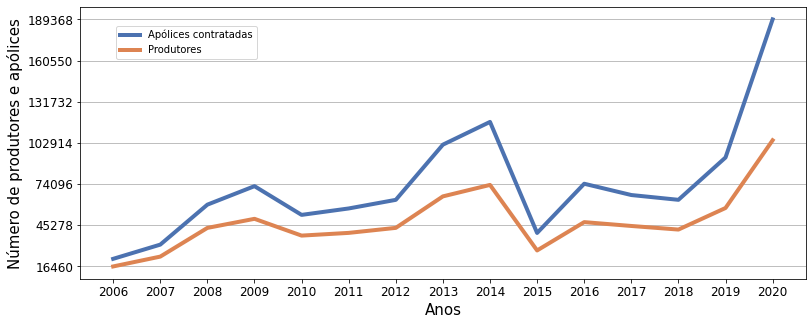
\includegraphics[width=0.8\textwidth]{figuras/apolices_produtores.png}\\
	%\small \textsuperscript {Fonte: Elaboração própria a partir de dados da Plataforma Atlas do Seguro Rural \cite{brasil21b}.}
    \parbox{\dimexpr\linewidth-3cm}{\raggedright
    \strut \textsuperscript{Fonte: Elaboração própria a partir de dados da Plataforma Atlas do Seguro Rural \cite{brasil21b}.}\strut}
    \label{apolices_produtores}
\end{figure}

É importante destacar que, no ano de $2021$, até o mês de junho, havia $66.928$ apólices contratadas \cite{brasil21}. Apesar do valor ser baixo se comparado ao ano de $2020$ ($189.368$ apólices), já é superior a $56,25\%$ dos anos anteriores. Padrão semelhante se observa com o número de produtores. No ano de $2021$, até o mês de junho haviam sido contabilizados $47.472$ produtores segurados \cite{brasil21b}.

%\subsubsection{Valores do prêmio e de subvenção ao prêmio de seguro rural}

O gráfico da Figura \ref{soma_ano_values} apresenta a evolução dos valores em milhões de reais de subvenção ao prêmio de seguro rural, prêmio pago pelo produtor e prêmio recebido pela seguradora entre $2006$ a $2020$. Observa-se que, com exceção do ano de $2014$, é possível notar uma tendência de crescimento dos valores de subvenção e prêmio pagos no período analisado. No ano de 2014, devido à contenções, o governo federal liberou apenas R\$ $400$ milhões dos R\$ $700$ milhões previstos para subsidiar o seguro rural. Esta contenção dos gastos governamentais pode ser um fator a ser considerado na queda dos valores do seguro rural ocorrida entre os anos de $2014$ e $2015$ \cite{andrade21}.

Em $2021$, até o mês de junho, o valor do prêmio pago à seguradora já havia alcançado R\$$1,25$ bilhões, o quarto maior valor registrado e cerca de $50,59\%$ maior que a média. O prêmio do produtor referente ao período de janeiro a junho de $2021$ já era equivalente a R$\$0,77$ bilhões, valor cerca de $69,67\%$ maior que a média do prêmio de responsabilidade do produtor. O valor concedido na forma de subvenção ao prêmio em $2021$ também é o quarto maior valor registrado, cerca de $25,96\%$ maior que a média dos valores de subvenção concedidos . Além disso, a partir do ano de $2016$, a parcela do prêmio sob responsabilidade do produtor passa a superar a parcela concedida pelo governo na forma de subvenção \cite{brasil21b}.

%\begin{figure}[H]
%	\centering
%	\caption{Valores do prêmio e de subvenção ao prêmio de seguro rural. Brasil $2006 - 2020$}
%	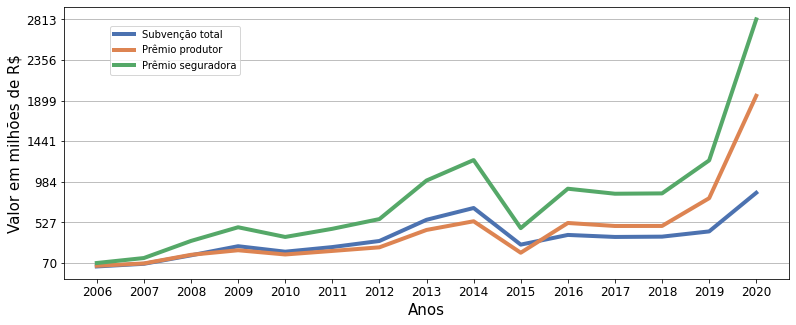
\includegraphics[width=0.8\textwidth]{figuras/soma_ano_values.png}\\
%	\small \textsuperscript {Fonte: Elaboração própria a partir de dados da Plataforma Atlas do Seguro Rural (Mapa, 2021).}
%    \label{soma_ano_values}
%\end{figure}

%\begin{figure}[H]
%	\centering
%	\caption{Soma da importância segurada (R\$ milhões). Brasil $2006 - 2020$}
%	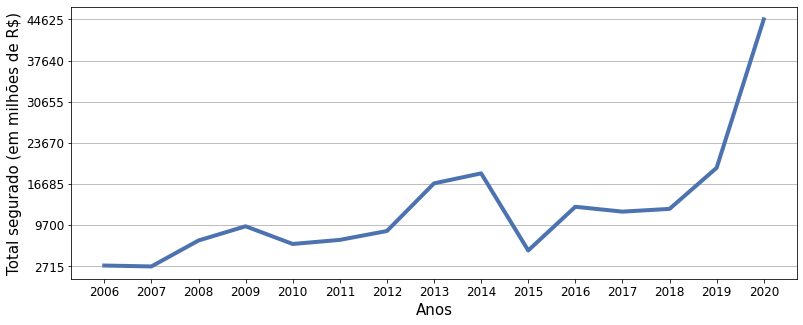
\includegraphics[width=0.8\textwidth]{figuras/total_segurado_mil.png}\\
%	\small \textsuperscript {Fonte: Elaboração própria a partir de dados da Plataforma Atlas do Seguro Rural (Mapa, 2021).}
%    \label{total_segurado_mil}
%\end{figure}

%\begin{figure}[H]
%	\centering
%	\caption{Total da área segurada em hectares. Brasil $2006 - 2020$}
%	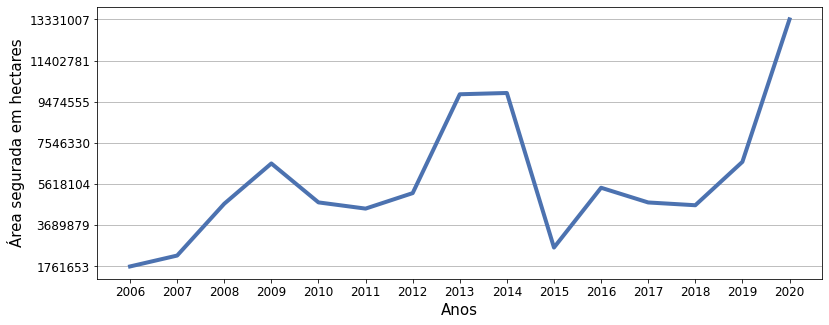
\includegraphics[width=0.8\textwidth]{figuras/area_segurada.png}\\
%	\small \textsuperscript {Fonte: Elaboração própria a partir de dados do Ministério da Agricultura, Pecuária e Abastecimento (MAPA).}
%    \label{area_segurada}
%\end{figure}

%\begin{figure}[H]
%	\centering
%	\caption{Número de apólices de seguro rural indenizadas. Brasil $2006 - 2019$}
%	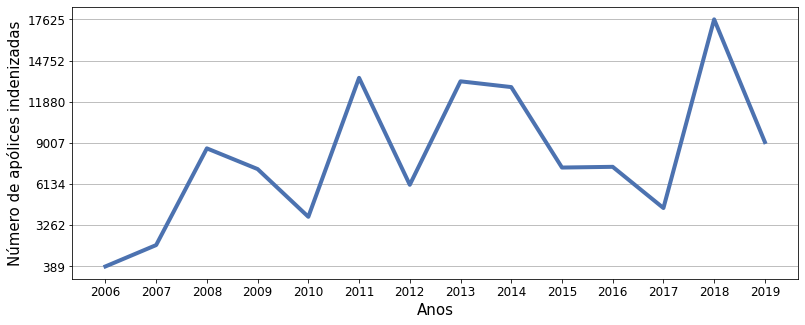
\includegraphics[width=0.8\textwidth]{figuras/apolices_indenizadas.png}\\
%	\small \textsuperscript {Fonte: Elaboração própria a partir de dados do Ministério da Agricultura, Pecuária e Abastecimento (MAPA)}
%    \label{apolices_indenizadas}
%\end{figure}

%\begin{figure}[H]
%	\centering
%	\caption{Valor das indenizações de seguro rural pagas (R\$ milhões). Brasil $2006 - 2019$}
%	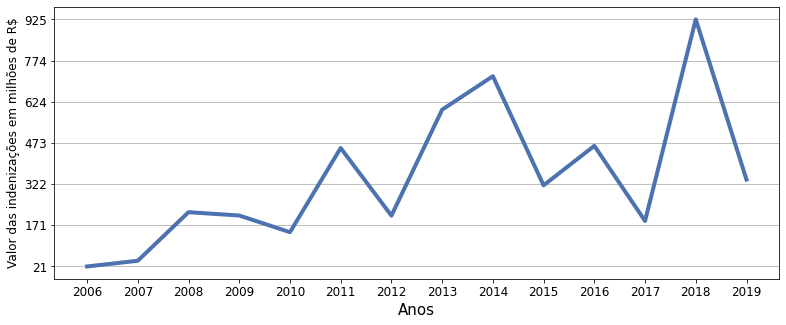
\includegraphics[width=0.8\textwidth]{figuras/valor_indenizacoes.png}\\
%	\small \textsuperscript {Fonte: Elaboração própria a partir de dados do Ministério da Agricultura, Pecuária e Abastecimento (MAPA)}
%    \label{valor_indenizacoes}
%\end{figure}

% variaveis_br
\begin{figure}[H]
	\centering
	\caption{Evolução das variáveis de seguro rural no Brasil}\label{variaveis_br}
	\small
	
	\subfloat[Valores do prêmio e de subvenção ao prêmio de seguro rural\label{soma_ano_values}]{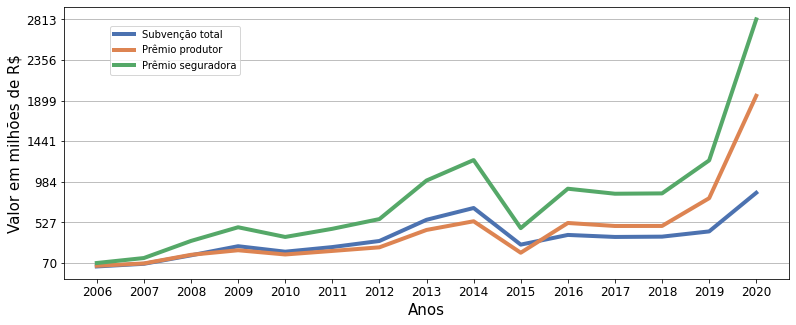
\includegraphics[width=0.45\textwidth]{figuras/soma_ano_values.png}}\hspace{0.1cm}
	\subfloat[Soma da importância segurada (R\$ milhões)\label{total_segurado_mil}]{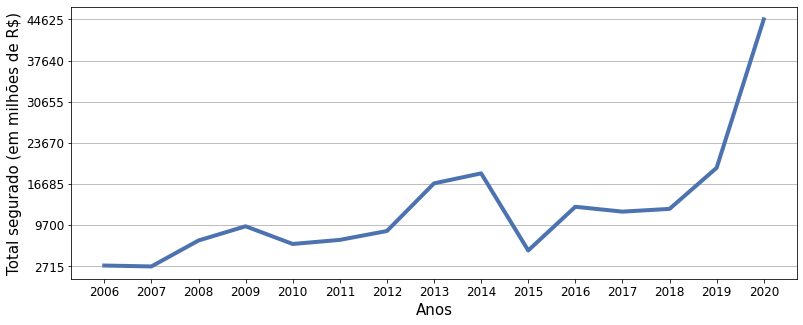
\includegraphics[width=0.45\textwidth]{figuras/total_segurado_mil.png}}\hspace{0.1cm}\\
	
	\subfloat[Total da área segurada em hectares.\label{area_segurada}]{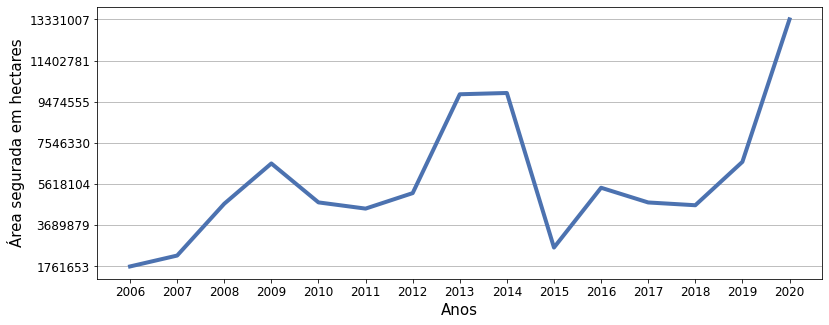
\includegraphics[width=0.45\textwidth]{figuras/area_segurada.png}}\hspace{0.1cm}
	\subfloat[Número de apólices de seguro rural indenizadas\label{apolices_indenizadas}]{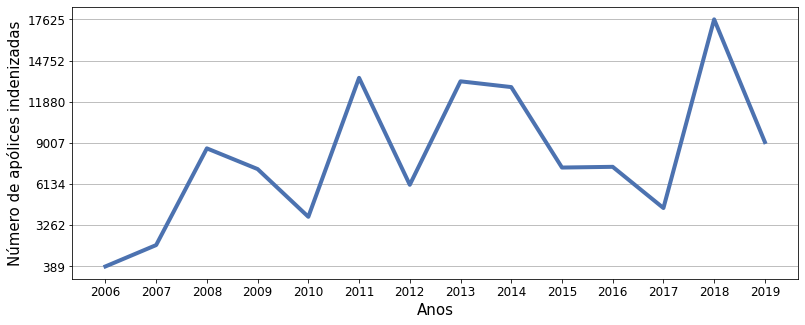
\includegraphics[width=0.45\textwidth]{figuras/apolices_indenizadas.png}}\\
	
	\subfloat[Valor das indenizações de seguro rural pagas (R\$ milhões)\label{valor_indenizacoes}]{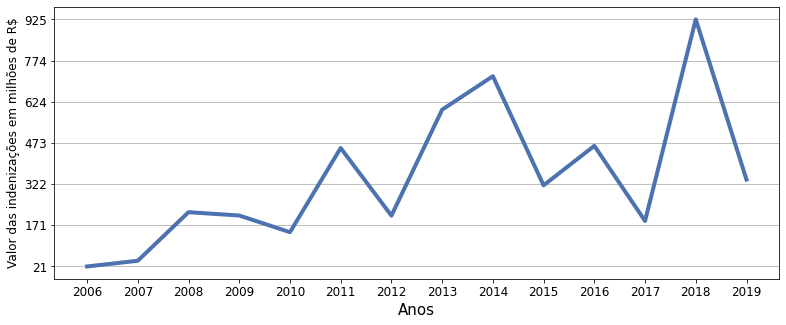
\includegraphics[width=0.45\textwidth]{figuras/valor_indenizacoes.png}}\hspace{0.1cm}
	\subfloat[Taxa média anual de contratação do prêmio de seguro rural\label{taxa_media}]{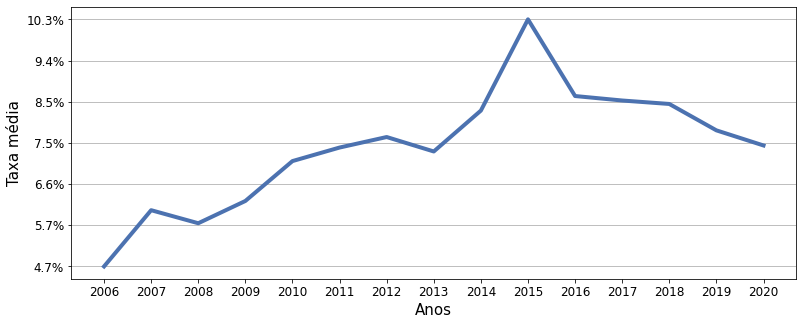
\includegraphics[width=0.45\textwidth]{figuras/taxa_media.png}}
	
	\parbox{\dimexpr\linewidth-2cm}{\raggedright
    \strut \textsuperscript{Fonte: Elaboração própria a partir de dados do Ministério da Agricultura, Pecuária e Abastecimento e da Plataforma
	Atlas do}\strut}\\
    \parbox{\dimexpr\linewidth-2cm}{\raggedright
    \strut \textsuperscript{Seguro Rural \cite{brasil21b}.}\strut}
\end{figure}

Os valores da soma da importância segurada em milhões de reais são apresentados no gráfico da Figura \ref{total_segurado_mil}. Observa-se que há crescimento dos valores segurados, com destaque para o crescimento entre os anos de $2019$ e $2020$, em que o os valores mais que duplicaram. Considerando o período entre $2006$ e $2020$, o crescimento da importância segurada foi de $15,55$ vezes o valor de $2006$. Também é possível observar que, entre os anos de $2014$ e $2015$, ocorreu uma queda de $70,68\%$ do valor segurado.  

Em $2020$, o Programa de Subvenção ao Prêmio do Seguro Rural (PSR) aplicou R\$ $880$ milhões, ou seja, o dobro do valor executado no ano de  $2019$. Para o ano de $2021$, a estimativa apresentada pelo Ministério da Agricultura e Abastecimento foi um aumento de R\$ $1$ bilhão a verba destinada ao PSR \cite{brasil21b}.

No ano de $2014$, o total segurado chegou a R$\$18.462,88$ milhões, no entanto, em $2015$ a soma da importância caiu para R$\$5.398,54$ milhões, o terceiro valor mais baixo do período. O valor mais alto ocorre no ano de $2020$, em que o valor segurado foi de R$\$45,7$ bilhões, o maior desde o início do programa em $2005$.

O valor da importância segurada alcançou $R\$14,4$ bilhões até o mês de junho de $2021$. Este valor é o quinto maior valor da série e já é maior que $25\%$ dos valores registrados nos anos anteriores \cite{brasil21b}. 

%\subsubsection{Área segurada em hectares}

A Figura \ref{area_segurada} apresenta o total da área segurada em hectares nos municípios do Brasil entre os anos de  $2006$ e  $2020$. É possível observar que, a área agrícola segurada no país praticamente dobrou entre $2019$ e $2020$, quando alcançou o maior valor, $13,7$ milhões de hectares, o que representou $20\%$ da área total agrícola do país. O aumento de área em relação a $2019$ é de $98\%$. O maior valor registrado em anos anteriores foi em $2014$, quando foram segurados $9,4$ milhões de hectares. No ano de $2021$, até o mês de junho, foram segurados cerca de $3,76$ milhões de hectares. Esse valor representa cerca de $71,76\%$ da área segurada em $2020$ \cite{brasil21b}. 

%\subsubsection{Indenizações}

Com relação ao número de indenizações,  o gráfico da Figura \ref{apolices_indenizadas} apresenta a evolução das apólices indenizadas ao longo do período analisado. O menor número de indenizações é $389$ em $2006$ e o maior valor ocorreu no ano de $2018$, sendo igual a $17.625$ indenizações. Durante o período, ocorre em média um número de $8.110$ apólices indenizadas por ano, sendo que o crescimento no número de apólices indenizadas foi de $23,31$ vezes entre $2006$ e $2019$. 

Os valores pagos como indenização entre os anos de $2006$ e $2019$ são apresentados no gráfico da Figura \ref{valor_indenizacoes} e variam entre R\$ $20.699.785,74$ em $2006$ e R\$ $924.988.210,45$ em $2018$. A média do valor das indenizações foi de R\$ $345.525.736,50$ no período analisado. 

%\begin{small}
%    \begin{table}[H]
%        \caption{Número de apólices de seguro rural indenizadas por regiões. Brasil $2006-2019$}\label{premio_regioes}
%         \input{../anexos/ap_indeniz_regioes.tex}
%    \end{table}
%\end{small}

%\subsubsection{Taxa média de contratação de seguro rural}

O gráfico apresentado na Figura \ref{taxa_media} mostra a trajetória da taxa de contratação do seguro rural. É possível constatar que a taxa se eleva, em média, de $4,7\%$ em $2006$ para $ 7,46\%$ em $2020$. Até o mês de junho de $2021$, o valor da taxa média havia alcançado $9,79\%$, o segundo maior valor da série, sendo superado pela taxa média cobrada em $2015$, que foi de $10,3\%$ \cite{brasil21b}.  

Segundo Santos e Silva (2017), espera-se que, à medida que o sistema de seguro rural se consolida, reduzam-se os preços das apólices devido aos ganhos de produtividade agropecuária e da redução de fatores de risco. Essas reduções podem ocorrer devido à adoção das orientações do zoneamento agrícola, de um maior conhecimento do histórico de eventos climáticos e dos sinistros ocorridos e, até mesmo em função da adoção de tecnologias, como o uso de irrigação etc. No entanto, essa redução das taxas não ocorreu no período analisado, como observado na Figura \ref{taxa_media}. 

%\begin{figure}[H]
%	\centering
%	\caption{Taxa média anual de contratação do prêmio de seguro rural. Brasil $2006 - 2020$}
%	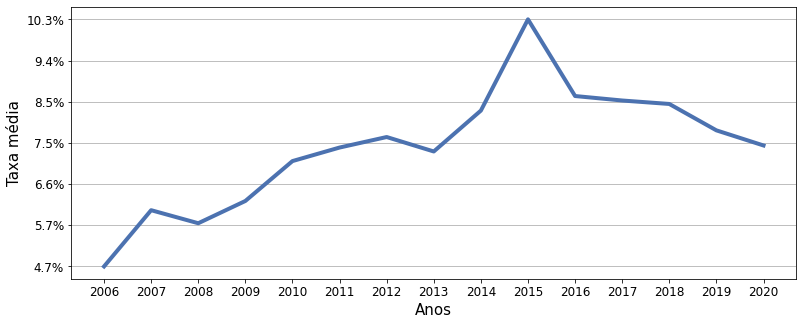
\includegraphics[width=0.8\textwidth]{figuras/taxa_media.png}\\
%	\small \textsuperscript {Fonte: Elaboração própria a partir de dados da Plataforma Atlas do Seguro Rural (Mapa, 2021).}
%   \label{taxa_media}
%\end{figure}

%\begin{small}
%\begin{table}[H]
%\caption{Taxa média de contratação do prêmio de seguro rural por regiões.  Brasil $2006-2020$}\label{tx_media_regioes}
% \input{../anexos/tx_media_regioes.tex}
%\end{table}
%\end{small}

%\subsubsection{Culturas}

A Figura \ref{percent_cult_apol} apresenta o percentual da participação das maiores culturas no número de apólices de seguro rural contratadas. A análise desse gráfico permite identificar que, com exceção de $2015$, a cultura da soja foi a que mais contratou seguro rural. Além disso, observa-se que o milho 2ª safra \footnote{Nesse caso o milho de 2ª safra é listado em separado devido aos distintos graus de risco em relação à 1ª safra \cite{santos17}.} tem cada vez mais aumentado sua participação no número de apólices contratadas. O milho 1ª safra, por sua vez, tem participação que varia entre $1,23\%$ e $16,46\%$, com média de  $6,16\%$ ao longo do período. A participação da cultura da maçã na contratação de seguro rural permanece relativamente estável ao longo do período, variando entre $8,79\%$ e $14,72\%$. 

\begin{figure}[H]
	\centering
	\caption{Percentual da participação das maiores culturas no número de apólices de seguro rural contratadas. Brasil $2006 - 2019$}
    	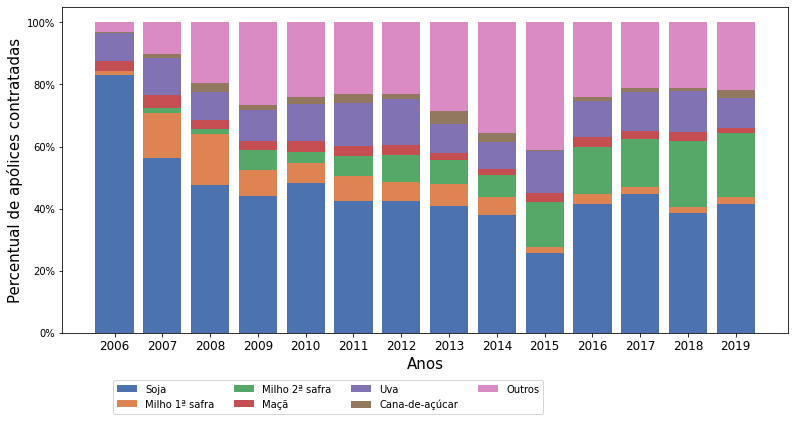
\includegraphics[width=0.8\textwidth]{figuras/percent_apolic_cult.png}\\
	%\small \textsuperscript {Fonte: Elaboração própria a partir de dados do Ministério da Agricultura, Pecuária e Abastecimento \cite{brasil21b}}
	\parbox{\dimexpr\linewidth-2.8cm}{\raggedright
    \strut \textsuperscript{Fonte: Elaboração própria a partir de dados do Ministério da Agricultura, Pecuária e Abastecimento \cite{brasil21b}.}\strut}
    \label{percent_cult_apol}
\end{figure}

A Tabela \ref{percent_culturas} apresenta a participação percentual de grupos de culturas em variáveis do seguro rural. É possível constatar que entre os anos de $2006$ e $2020$, as culturas de grãos foram responsáveis por $74,85\%$ das apólices contratadas, seguida das culturas de frutas com $14,74\%$ das apólices no período. Em terceiro lugar está a cultura de olerícolas, com cerca de $3,36\%$ de participação na contratação de apólices de seguro rural. Uma estrutura semelhante de participação percentual de grupos de culturas pode ser observada com relação à participação no valor total segurado. O grupo de cultura que mais se destaca é a dos grãos, com $74,88\%$ do total segurado, seguido das frutas e do café, com $9,55\%$ e $4,04\%$, respectivamente. 

\begin{small}
\begin{table}[H]
\caption{Participação percentual das culturas nos valores do seguro rural. Brasil $2006-2020$}\label{percent_culturas}
 \footnotesize
\vspace{0.05cm}
\begin{tabularx}{\textwidth}{lRRRRR}
    \hline \\[-1.9ex]	 
    Cultura    & \% das apólices & \% do total segurado & \% do premio total & \% de subvenção & Taxa média \\
    \hline \\[-1.9ex]	 
    Grãos      & 74,85\%         & 74,88\%              & 78,86\%            & 77,35\%         & 7,70\%     \\
    Frutas     & 14,74\%         & 9,55\%               & 13,14\%            & 16,07\%         & 9,17\%     \\
    Olerícolas & 3,36\%          & 2,74\%               & 3,17\%             & 2,85\%          & 7,64\%     \\
    Café       & 3,07\%          & 4,04\%               & 2,19\%             & 1,61\%          & 3,15\%     \\
    Cana       & 2,08\%          & 2,98\%               & 0,77\%             & 0,69\%          & 1,63\%     \\
    Pecuária   & 0,73\%          & 1,16\%               & 0,77\%             & 0,32\%          & 3,26\%     \\
    Floresta   & 0,30\%          & 3,51\%               & 0,42\%             & 0,35\%          & 1,60\%     \\
    Outros     & 0,88\%          & 1,13\%               & 0,68\%             & 0,75\%          & 4,64\%     \\ 
    \hline 
\end{tabularx}
%\vspace{0.5cm}
\small \textsuperscript{Fonte: Elaboração própria a partir de dados da Plataforma Atlas do Seguro Rural (Mapa, 2021).  }\\
\end{table}
\end{small}

Além disso, é possível observar na Tabela \ref{percent_culturas}, os percentuais de subvenção ao prêmio de seguro rural e os valores da taxa média de contratação do seguro. As taxas cobradas durante o período para a cultura de grãos foi de $7,70\%$, a taxa cobrada das culturas de frutas foi de $9,17\%$ e as olerícolas tiveram uma taxa média de contratação de $7,64\%$. Os percentuais de subvenção dessas culturas são, também, os mais altos: $77,35\%$ de subvenção para os grãos, $16,07\%$ para as culturas de frutas e $2,85\%$ para as olerícolas. Ou seja, os grupos de culturas com maior demanda pelo seguro, além de apresentarem os maiores valores de apólices, os maiores valores e maior ocorrência de sinistros, são também aqueles com maiores taxas médias. 

De acordo com  Santos e Silva (2017), este fato pode apontar para a possibilidade de dois fenômenos a serem melhor examinados. O primeiro diz respeito à situação em que as maiores taxas resultam do fato de que maiores subvenções são dadas a cultivos de maior risco. O segundo fenômeno possível é que as taxas sejam mais altas, principalmente no caso dos produtores que adotam o ZARC, com elevada tecnologia produtiva, alta produtividade e não têm estas características levadas em consideração como informação que contribui para a redução das taxas. Dessa forma, se por um lado o seguro agrícola não se consolida sem a subvenção dada pelo Estado, por outro, é possível que esse sistema de subvenção ao prêmio crie distorções no mercado de seguro rural. 

%\subsubsection{Seguradoras}

A Tabela \ref{seguradoras} exibe a distribuição das fatias de mercado das seguradoras entre $2006$ e $2020$. Apesar de as seguradoras passarem de cinco, em $2006$, para $16$ companhias aptas a operar com seguro rural em $2020$, é possível constatar que há uma concentração do mercado de seguro em um número reduzido de seguradoras. 

\begin{small}
\begin{table}[H]
\caption{Participação de mercado das seguradoras. Brasil $2006-2020$}\label{seguradoras}
 \footnotesize
\vspace{0.05cm}
\begin{tabularx}{\textwidth}{lRRRRRRR}
    \hline \\[-1.9ex]	 
    Seguradora         & Apólices        & \% do número de apólices  & Beneficiários  & \% dos beneficiários  & Área segurada (em mil ha)  & \% de área segurada   \\
    \hline \\[-1.9ex]	 
    Brasilseg         &  $410.892$      &  $37,23  $                &  $95.769$                    &  $26,85  $            &  $48.076,26$       & $55,31  $              \\
    Mapfre            &  $149.389$      &  $13,54  $                &  $49.274$                    &  $13,82  $            &  $7.309,17$        &  $8,41  $               \\
    Essor             &  $119.087$      &  $10,79  $                &  $38.995$                    &  $10,93  $            &  $4.603,47$        &  $5,30  $               \\
    Swiss Re          &  $91.410$       &  $8,28  $                 &  $34.483$                    &  $9,67  $             &  $7.870,31$        &  $9,06  $               \\
    Nobre             &  $82.500$       &  $7,48  $                 &  $29.053$                    &  $8,15  $             &  $2.747,88$        &  $3,16  $               \\
    Allianz           &  $66.983$       &  $6,07  $                 &  $21.210$                    &  $5,95  $             &  $5.387,98$        &  $6,20  $               \\
    Sancor            &  $49.567$       &  $4,49  $                 &  $22.516$                    &  $6,31  $             &  $3.210,37$        &  $3,69  $               \\
    Fairfax           &  $35.343$       &  $3,20  $                 &  $18.349$                    &  $5,14  $             &  $2.055,87$        &  $2,37  $               \\
    Porto Seguro      &  $26.306$       &  $2,38  $                 &  $6.152$                     &  $1,72  $             &  $259,33$          &  $0,30  $               \\
    Newe              &  $22.741$       &  $2,06  $                 &  $12.337$                    &  $3,46  $             &  $1.469,10$        &  $1,69  $               \\
    Tokio Marine      &  $19.808$       &  $1,79  $                 &  $11.263$                    &  $3,16  $             &  $1.722,64$        &  $1,98  $               \\
    Too               &  $14.844$       &  $1,35  $                 &  $9.768$                     &  $2,74  $             &  $1.163,48$        &  $1,34  $               \\
    Aliança do Brasil &  $7.200$        &  $0,65  $                 &  $3.294$                     &  $0,92  $             &  $593,19$          &  $0,68  $               \\
    Excelsior         &  $4.472$        &  $0,41  $                 &  $2.292$                     &  $0,64  $             &  $238,97$          &  $0,27  $               \\
    Sompo             &  $3.062$        &  $0,28  $                 &  $1.901$                     &  $0,53  $             &  $181,66$          &  $0,21  $               \\
    Itaú              &  $9$            &  $0,00  $                 &  $9$                         &  $0,00  $             &  $25,10$           &  $0,03  $               \\
    \hline \\[-1.9ex]
    \textbf{Total}    & \textbf{1.103.613} & \textbf{100  }         & \textbf{213.692}             & \textbf{100  }        & \textbf{86.914,79} & \textbf{100  }\\
	\hline 
\end{tabularx}
%\vspace{0.5cm}
\small \textsuperscript{Fonte: Elaboração própria a partir de dados da Plataforma Atlas do Seguro Rural (Mapa, 2021).}\\
\footnotesize{Nota: Valores acumulados $2006 -- 2020$}\\
\end{table}
\end{small}

Ao se analisar a participação no percentual do número de apólices de seguro rural, percebe-se que apenas as três maiores seguradoras (Brasilseg, Mapfre e Essor) concentram cerca de $61,56\%$ do mercado. Com relação ao percentual dos beneficiários, as três maiores seguradoras contam com cerca de $51,60\%$ dos beneficiários durante o período analisado. A concentração é ainda maior quando se analisa o percentual da área segurada, sendo que a  maior seguradora do ramo (Brasilseg) conta com um percentual de $55,31\%$ da área segurada em hectares. As três maiores seguradoras são responsáveis pelo seguro de $72,78\%$ da área segurada. 

%A próxima seção tem como objetivo apresentar os resultados da análise da distribuição espacial dos dados do seguro rural no Brasil. 

\subsection{A DISTRIBUIÇÃO REGIONAL DO SEGURO RURAL} 

Os gráficos apresentados na Figura \ref{variaveis_regioes} exibem a evolução, entre os anos de $2006$ e $2019$, das variáveis de seguro rural analisadas por regiões.

Na figura \ref{ap_contrat_regioes}, é possível observar a evolução do número de apólices contratadas nas regiões brasileiras. Na Figura \ref{ap_contrat_regioes}, observa-se que a região Sul se destaca das demais com relação ao número de apólices contratadas. O menor número de apólices contratadas na região Sul foi de $16.525$ apólices no ano de $2006$. O valor médio de apólices contratadas durante o período foi $44.166$ apólice. No ano de $2014$, foi registrado o maior número de apólices contratadas ($76.668$ apólices). 

% variaveis_regioes
\begin{figure}[H]
	\centering
	\caption{Evolução das variáveis de seguro rural por regiões. Brasil $2006 - 2019$}\label{variaveis_regioes}
	\small
	
	\subfloat[Número de apólices contratadas\label{ap_contrat_regioes}]{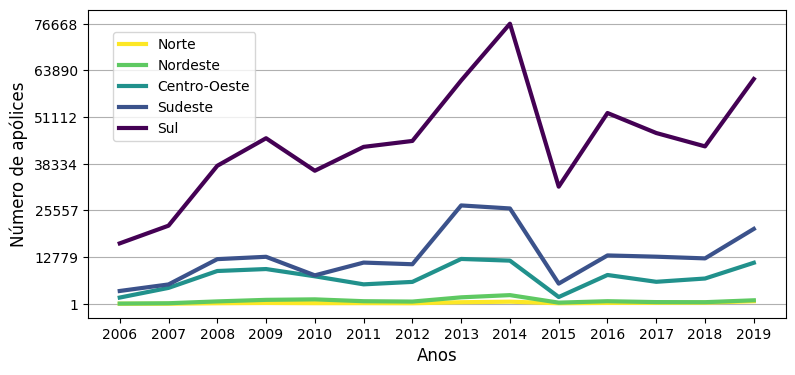
\includegraphics[width=0.45\textwidth]{figuras/ap_contrat_regioes.png}}\hspace{0.1cm}
	\subfloat[Total segurado (em milhões de R\$)\label{t_segurado_regioes}]{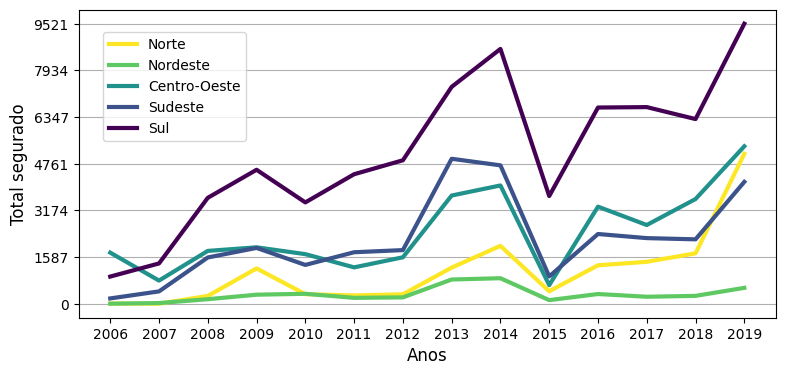
\includegraphics[width=0.45\textwidth]{figuras/t_segurado_regioes.png}}\\
	
	\subfloat[Valores de prêmio (em milhões de R\$)\label{soma_premio_regioes}]{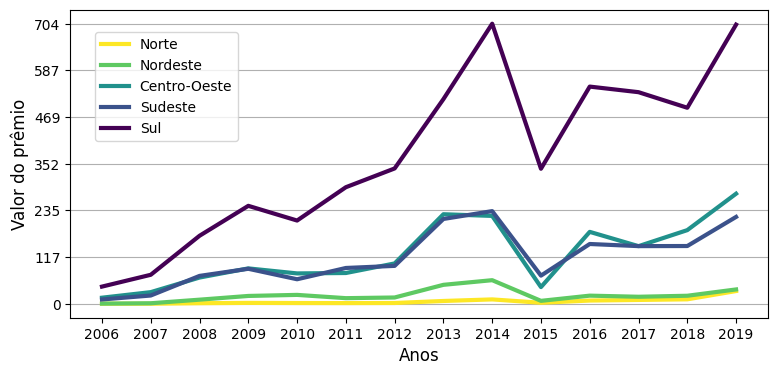
\includegraphics[width=0.45\textwidth]{figuras/soma_premio_regioes.png}}\hspace{0.1cm}
	\subfloat[Valores subvenção (em milhões de R\$)\label{t_subvencao_regioes}]{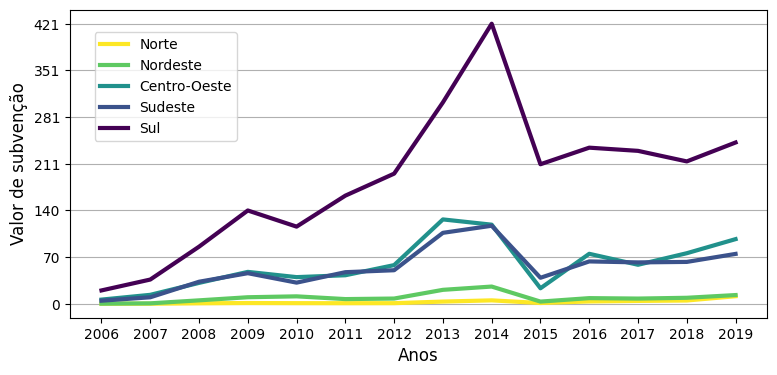
\includegraphics[width=0.45\textwidth]{figuras/t_subvencao_regioes.png}}\\
	
	\subfloat[Apólices indenizadas\label{ap_indeniz_regioes}]{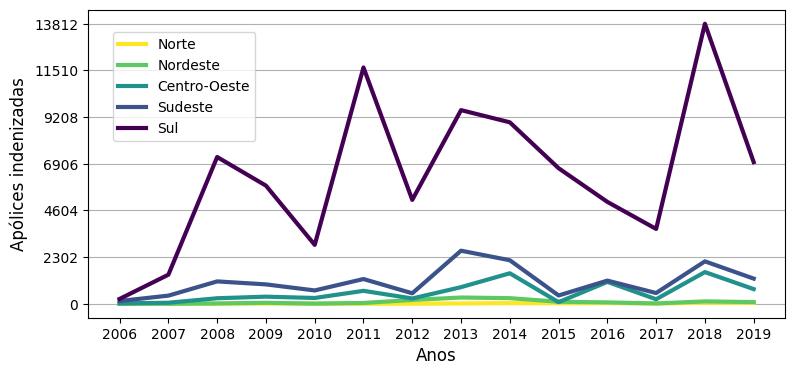
\includegraphics[width=0.45\textwidth]{figuras/ap_indeniz_regioes.png}}\hspace{0.1cm}
	\subfloat[Valor das indenizações (em milhões de R\$)\label{inde_pagas_regioes}]{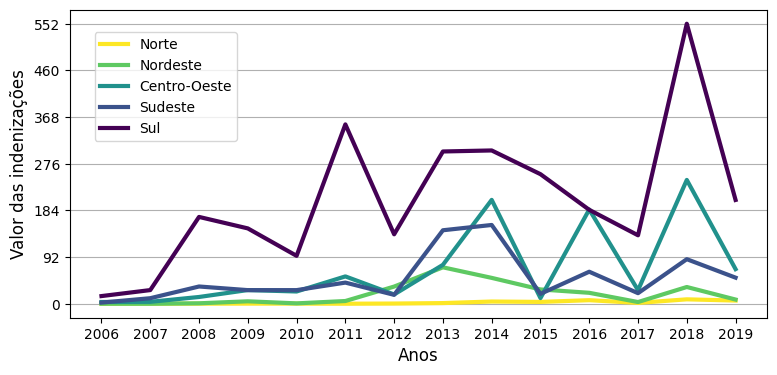
\includegraphics[width=0.45\textwidth]{figuras/inde_pagas_regioes.png}}\\
	
    \parbox{\dimexpr\linewidth-2cm}{\raggedright
    \strut \textsuperscript{Fonte: Elaboração própria a partir de dados do Ministério da Agricultura, Pecuária e Abastecimento \cite{brasil21b}}\strut}
\end{figure}

A segunda região com maior número de apólices contratadas é a região Sudeste (Figura \ref{ap_contrat_regioes}). Em média, na região Sudeste, foram contratadas $12.942$ apólices por ano, o maior valor registrado foi $26.913$ apólices contratadas em $2013$. A região Centro-Oeste é a terceira região com mais apólices contratadas, sendo que em média foram contratadas $7.225$  por ano e, em $2013$ foi registrado o maior número de apólices ($12.260$). Por fim, as regiões Norte e Nordeste, apresentaram respectivamente, em média, $240$ e $804$ apólices contratadas por ano.

A taxa de crescimento do número de apólices contratadas na região sul foi de $3,72$ vezes o valor inicial entre os anos $2006$ e $2019$. Por sua vez, durante o período analisado a região Sudeste teve um crescimento do número apólices de $5,87$ vezes e a região Centro-Oeste apresentou um crescimento do número de apólices de $6,66$ vezes. As regiões Norte e Nordeste apresentaram um crescimento médio anual igual a $0,14\%$ e $4,04\%$ respectivamente. 

Ao se analisar a evolução do total segurado nas regiões brasileiras apresentado na Figura \ref{t_segurado_regioes}, é possível observar que a região Sul se destaca com, em média, $5146,83$ milhões de valor segurado total. O maior valor foi registrado em $2019$ e foi igual a $9520,85$ milhões, o segundo maior valor foi igual a $8664,31$ milhões e foi registrado em $2015$. 

No início da série valores a região Centro-Oeste apresenta um maior valor total segurado do que a região Sul (5.355 milhões). Além disso, como é possível observar na Figura \ref{t_segurado_regioes}, a partir do ano de $2016$ a região Centro-Oeste supera a região Sudeste no valor total segurado. A região Norte apresentou, com relação ao total segurado, os valores de $120,35$ milhões em $2009$ e $197,01$ milhões em $2014$. 
Além disso, a região Norte apresenta o seu maior valor no ano de $2019$, com total segurado igual a $509,94$ milhões. Também é possível observar que há indícios de haver um crescimento do total segurado em todas as regiões. 

O total segurado na região Sul apresenta um crescimento de cerca de $10,27$ vezes entre os anos de $2006$ e $2019$. Na região Sudeste, o crescimento foi de $22,52$ vezes o valor registrado em $2006$. Por sua vez, o Centro-Oeste apresentou um crescimento de cerca de $3,07$ vezes o valor do total segurado durante o período. O valor do total segurado na região Norte cresceu $499.51$ vezes entre os anos $2006$ e $2019$. Por fim, no Nordeste, o valor total segurado apresentou um crescimento de $106,95$ vezes o valor inicial. 

Para mais, ao se analisar a Figura \ref{soma_premio_regioes} e \ref{t_subvencao_regioes}, é possível observar que as variáveis valores de prêmio e valores subvenção apresentam crescimento durante o período analisado. Também é possível observar que, com exceção das variáveis relacionadas à indenização, as variáveis apresentam uma queda entre os anos de $2014$ e $2015$.

É possível observar na Figura \ref{ap_indeniz_regioes}, que a região Sul se destaca quando se analisa o número de apólices indenizadas. Os valores variam de $237$ em $2006$ e $13812$ apólices indenizadas em $2019$. Em média, a região Sul teve cerca de $6364$ apólices indenizadas durante o período. Além disso, durante os anos analisados, houve um crescimento de $58,28\%$ no número de apólices de seguro rural indenizadas. A região Sudeste é a segunda região com maior número de apólices indenizadas, sendo que o menor número de apólices indenizadas na região Sudeste foi de $135$ e ocorreu em $2006$, com maior valor registrado em $2013$, equivalente a $2.616$. 

Ao longo dos anos analisados, a diferença entre o número de apólices na região Sul e Sudeste foi em média igual a $5.283$ apólices. A região Centro-Oeste foi responsável por, em média, $559,64$ apólices indenizadas. O maior número de apólices indenizadas na região Centro-Oeste foi registrado em $2018$ e foi igual a $1561$ apólices. As regiões Norte e Nordeste tiveram em média $15,57$ e $88,64$, respectivamente. 

Com relação ao valor das indenizações de seguro rural pagas, é possível observar na Figura \ref{inde_pagas_regioes}, que a região Sul é a que possui os maiores valores pagos como indenização. Em média, foram pagos R$\$205,66$ milhões como indenização. O maior valor foi equivalente a R$\$551,74$ milhões e foi registrado em $2018$ e o menor valor foi registrado no primeiro ano analisado, sendo equivalente a R$\$15.06$ milhões. 

A Tabela \ref{media_regioes} apresenta a média dos valores anuais das variáveis de seguro rural acumulados por regiões no Brasil no período de $2006$ e $2019$. Como é possível observar, que a região Sul se destaca das demais com os maiores valores das médias das variáveis. Com relação ao número de apólices contratadas, a segunda região com maior média da variável total de apólices contratadas é o Sudeste. No entanto, quando se analisa a média da soma da importância seguradas, a segunda região com maior média é a região Centro-Oeste. A região Centro-Oeste, também conta com maiores médias nas variáveis soma dos prêmios pagos, total da subvenção e soma das indenizações pagas com relação às regiões Norte, Nordeste e Sudeste. A região Sudeste apresenta a maior média anual do número de apólices indenizadas. 



\begin{small}
\begin{table}[H]
\caption{Média anual dos valores das variáveis de seguro rural por regiões. Brasil $2006-2019$}\label{media_regioes}
\begin{center}
\footnotesize
    \begin{tabular}{lrrrrr}
    \hline \\[-1.9ex]	
    Variável                                  & Norte   & Nordeste & Centro-Oeste & Sudeste  & Sul       \\
    \hline \\[-1.9ex]	
    Total de apólices contratada              &  240,14 &   803,57 &      7.225,36 &  12.941,5 &  44.166,14 \\
    Soma da importância segurada (R\$ milhão) &   111,5 &   319,82 &      2.428,79 &  2.178,54 &   5.146,84 \\
    Soma dos prêmios (R\$ milhão)             &    6,37 &    20,76 &       123,43 &   115,02 &    371,72 \\
    Total de subvenção (R\$ milhão)           &    2,66 &     9,25 &        58,25 &    53,52 &    186,56 \\
    Soma das indenizações pagas (R\$ milhão)  &    2,39 &    18,73 &        68,59 &    50,15 &    205,66 \\
    Taxa média aplicada às apólices           &    0,01 &     0,01 &         0,13 &     0,11 &      0,45 \\
    Número de apólices indenizadas            &   15,57 &    88,64 &       559,64 &  1.081,57 &   6.364,57 \\
    \hline 
    \end{tabular}
\end{center}
\small \textsuperscript {Fonte: Elaboração própria a partir de dados do Ministério da Agricultura, Pecuária e Abastecimento (MAPA)}\\


\end{table}
\end{small}

A média dos valores anuais da taxa média de contratação de apólices indica que, a região Sul é a que possui maior taxa de contratação de seguro com taxa média igual a $0,45$ ao longo dos anos. A região Centro-Oeste é a que tem o segundo maior valor de taxa média durante os anos, sendo igual a $0,13$. As regiões Norte e Nordeste apresentaram taxa média igual a $0,01$.

\subsection{DISTRIBUIÇÃO ESPACIAL DO SEGURO RURAL}

A análise da distribuição espacial das variáveis se inicia com a visualização dos mapas temáticos. Por meio destes mapas, busca-se identificar visualmente se há a ocorrência de padrões na distribuição espacial das variáveis do seguro rural.

O primeiro grupo de mapas, apresentado na Figura \ref{map_segurado}, exibe a distribuição espacial da soma da importância segurada (R\$ milhão) nos municípios brasileiros entre os anos de $2006$ e $2019$. Para a construção dos mapas, os valores da variável foram divididos em 5 intervalos \footnote{Para a criação dos intervalos foi aplicado algoritmo Fisher Jenks aos valores das variáveis diferentes de $0$ e os intervalos foram criados tendo como referência os valores do ano de 2019 \cite{jenks77}}.

\begin{figure}[H]
	\centering
	\caption{Total segurado por municípios (em mil R\$). Brasil $2006 - 2019$}
	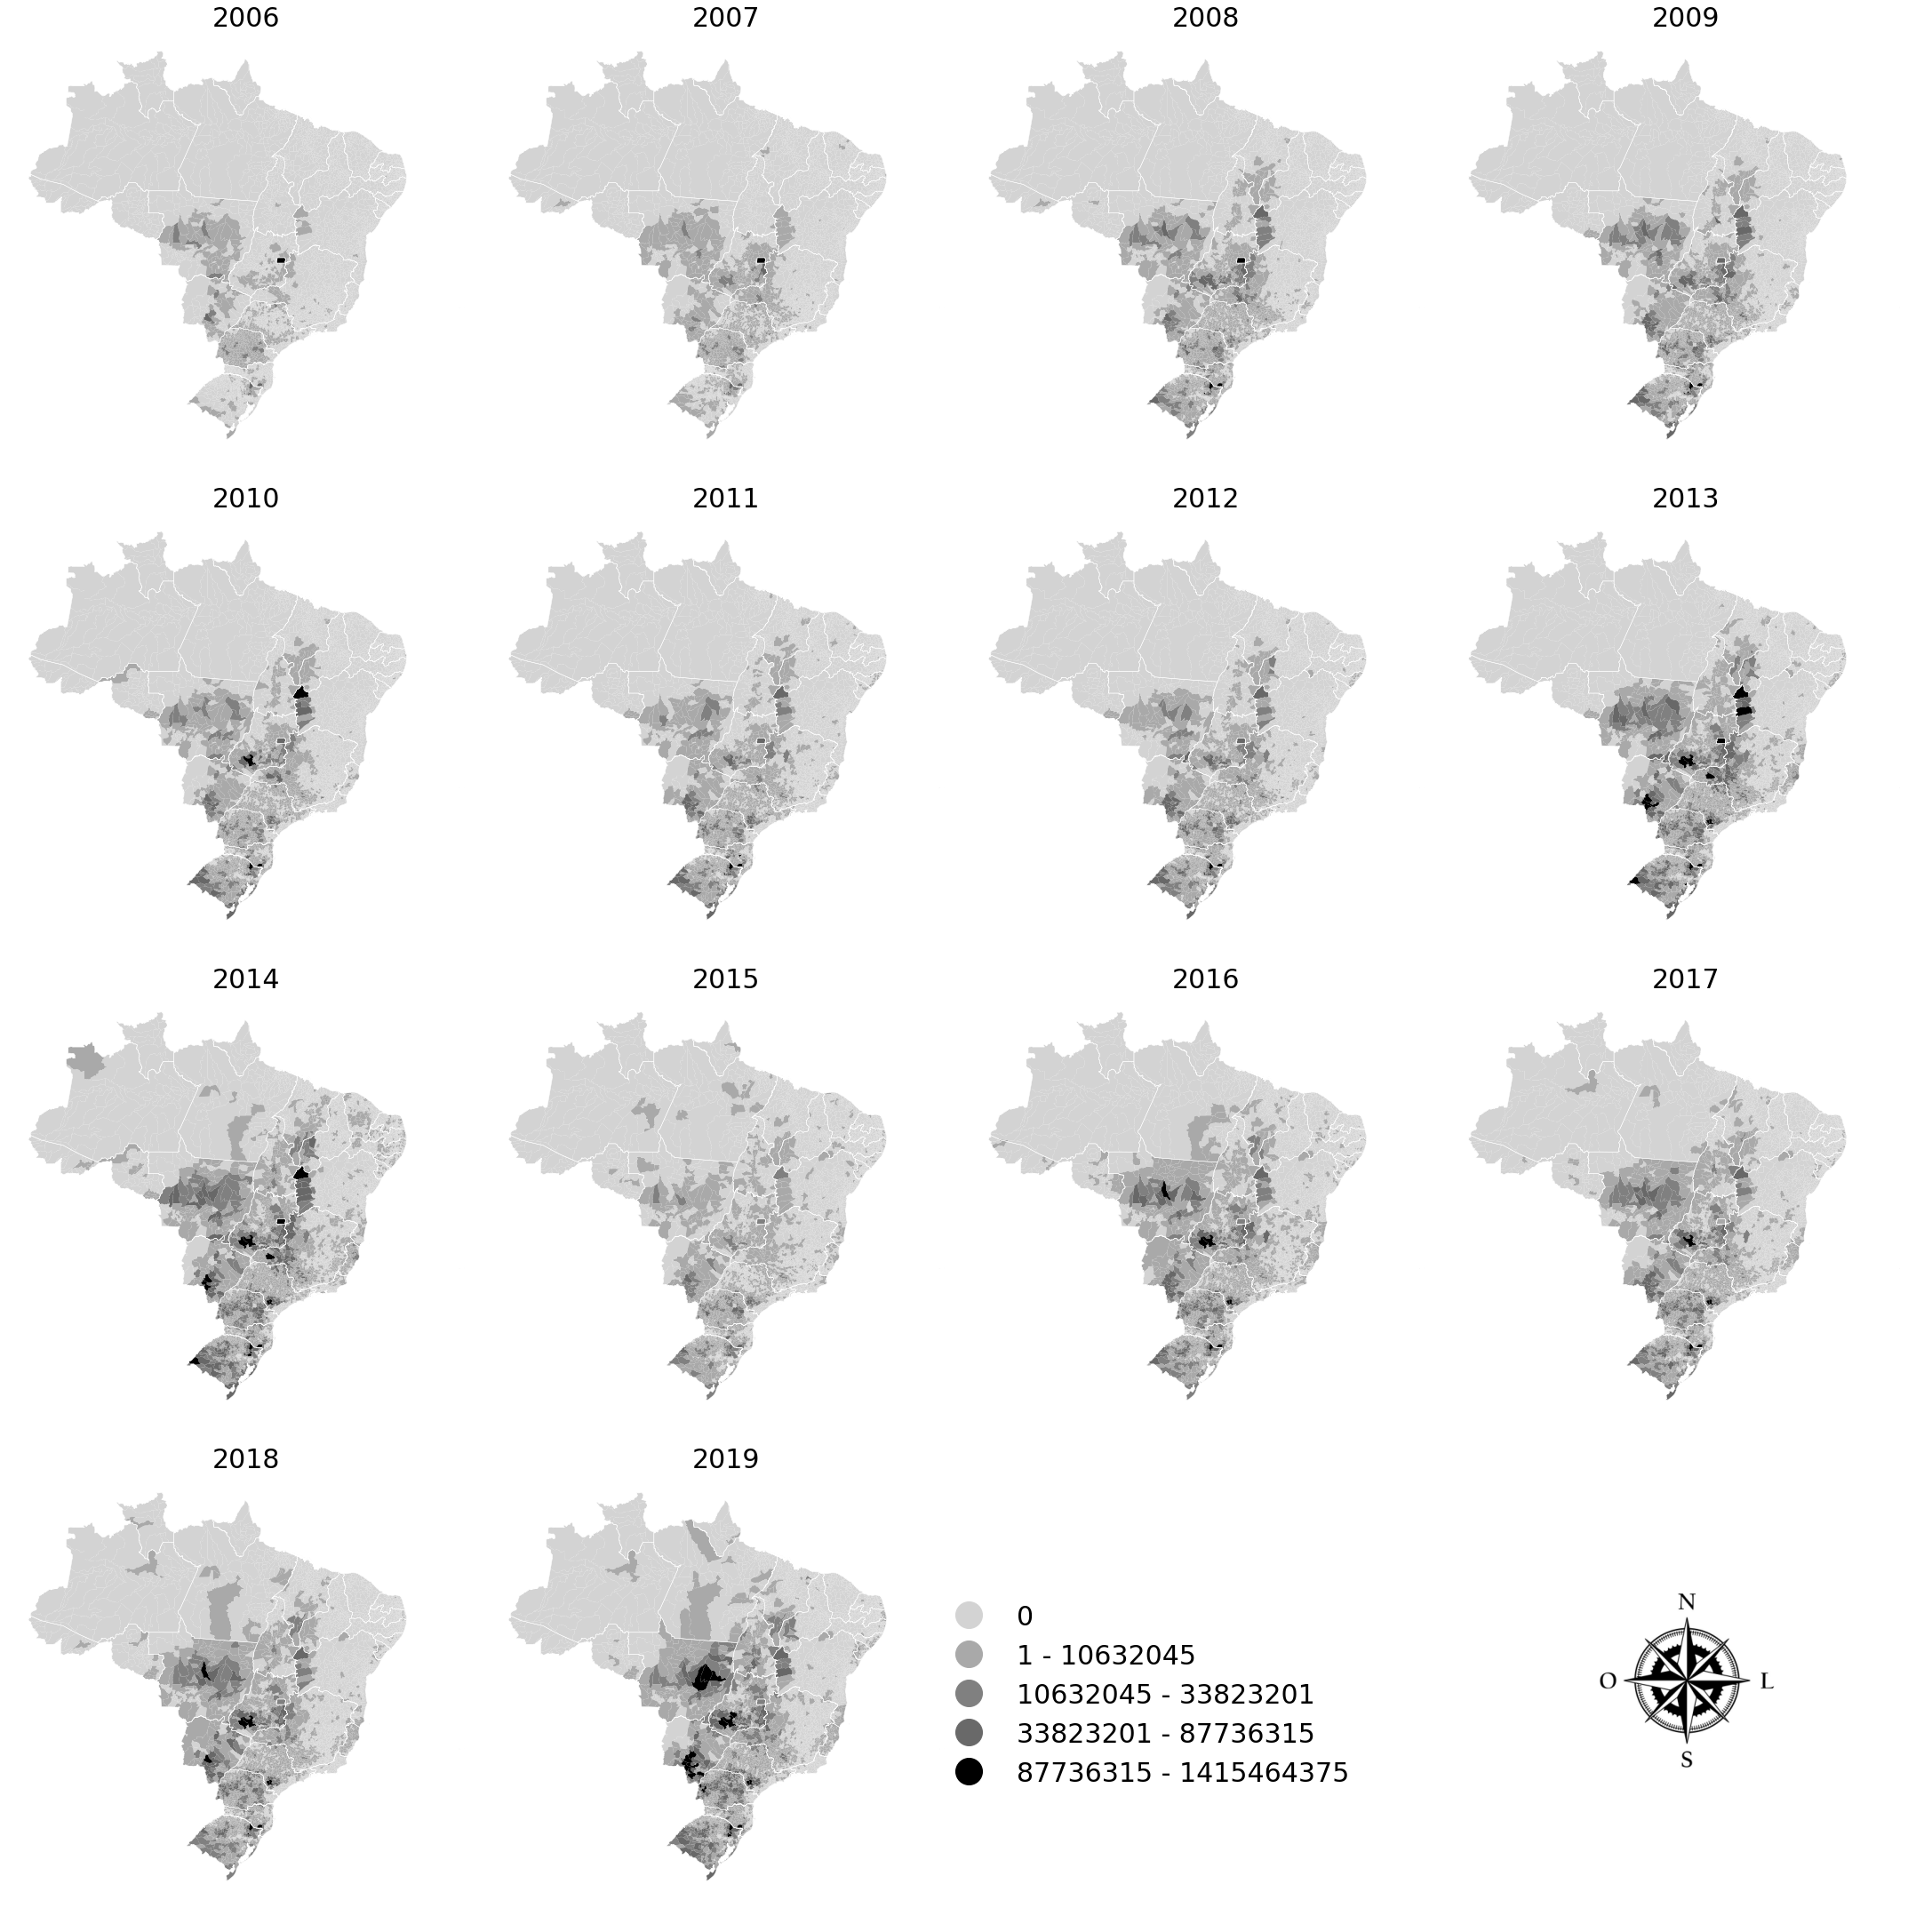
\includegraphics[width=0.9\textwidth]{figuras/map_total_segurado_mil.png}
	\small \textsuperscript {Fonte: Elaboração própria a partir de dados do Ministério da Agricultura, Pecuária e Abastecimento \cite{brasil21b}}
    \label{map_segurado}
\end{figure}

Pela análise da Figura \ref{map_segurado}, é possível observar que a distribuição espacial do total segurado se modificou no decorrer dos anos, apesar de se concentrar principalmente nas Regiões Sul e Centro-Oeste. É possível também destacar que, durante o período analisado, há indícios de concentrações espaciais na região do Extremo Oeste Baiano no Estado da Bahia, Sudoeste de Mato Grosso do Sul, Sul Goiano no Estado de Goiás e Sudeste, no sul do Estado de São Paulo.

O conjunto de mapas apresentado na Figura \ref{map_apolices}, exibe o número de apólices de seguro rural contratadas por municípios entre $2006$ e $2019$. Ao longo dos anos, o número de municípios com nenhuma apólice contratada cai e há indícios de um aumento do número de apólices até o ano de $2014$. Entre os anos de $2014$ e $2015$, há uma queda no número de apólices contratadas, como já foi mostrado no gráfico da Figura \ref{apolices_produtores}, e das demais variáveis relacionadas ao seguro rural. Essa redução também pode ser visualizada no mapa da Figura \ref{map_apolices}, em que o ano de $2015$ apresenta municípios com menor número de apólices contratadas. 

Ao se analisar a distribuição espacial, observa-se que há indícios de haver uma maior concentração espacial do total segurado e do número de apólices de seguro rural contratadas em algumas regiões. A partir do ano de $2015$ a retomada do crescimento destas variáveis (Figura \ref{total_segurado_mil}) pode ser visualizado com um maior número de áreas de coloração mais escura nos mapas (Figuras \ref{map_segurado} e \ref{map_apolices}).

\begin{figure}[H]
	\centering
	\caption{Número de apólices de seguro rural contratadas por municípios. Brasil $2006 - 2019$}
	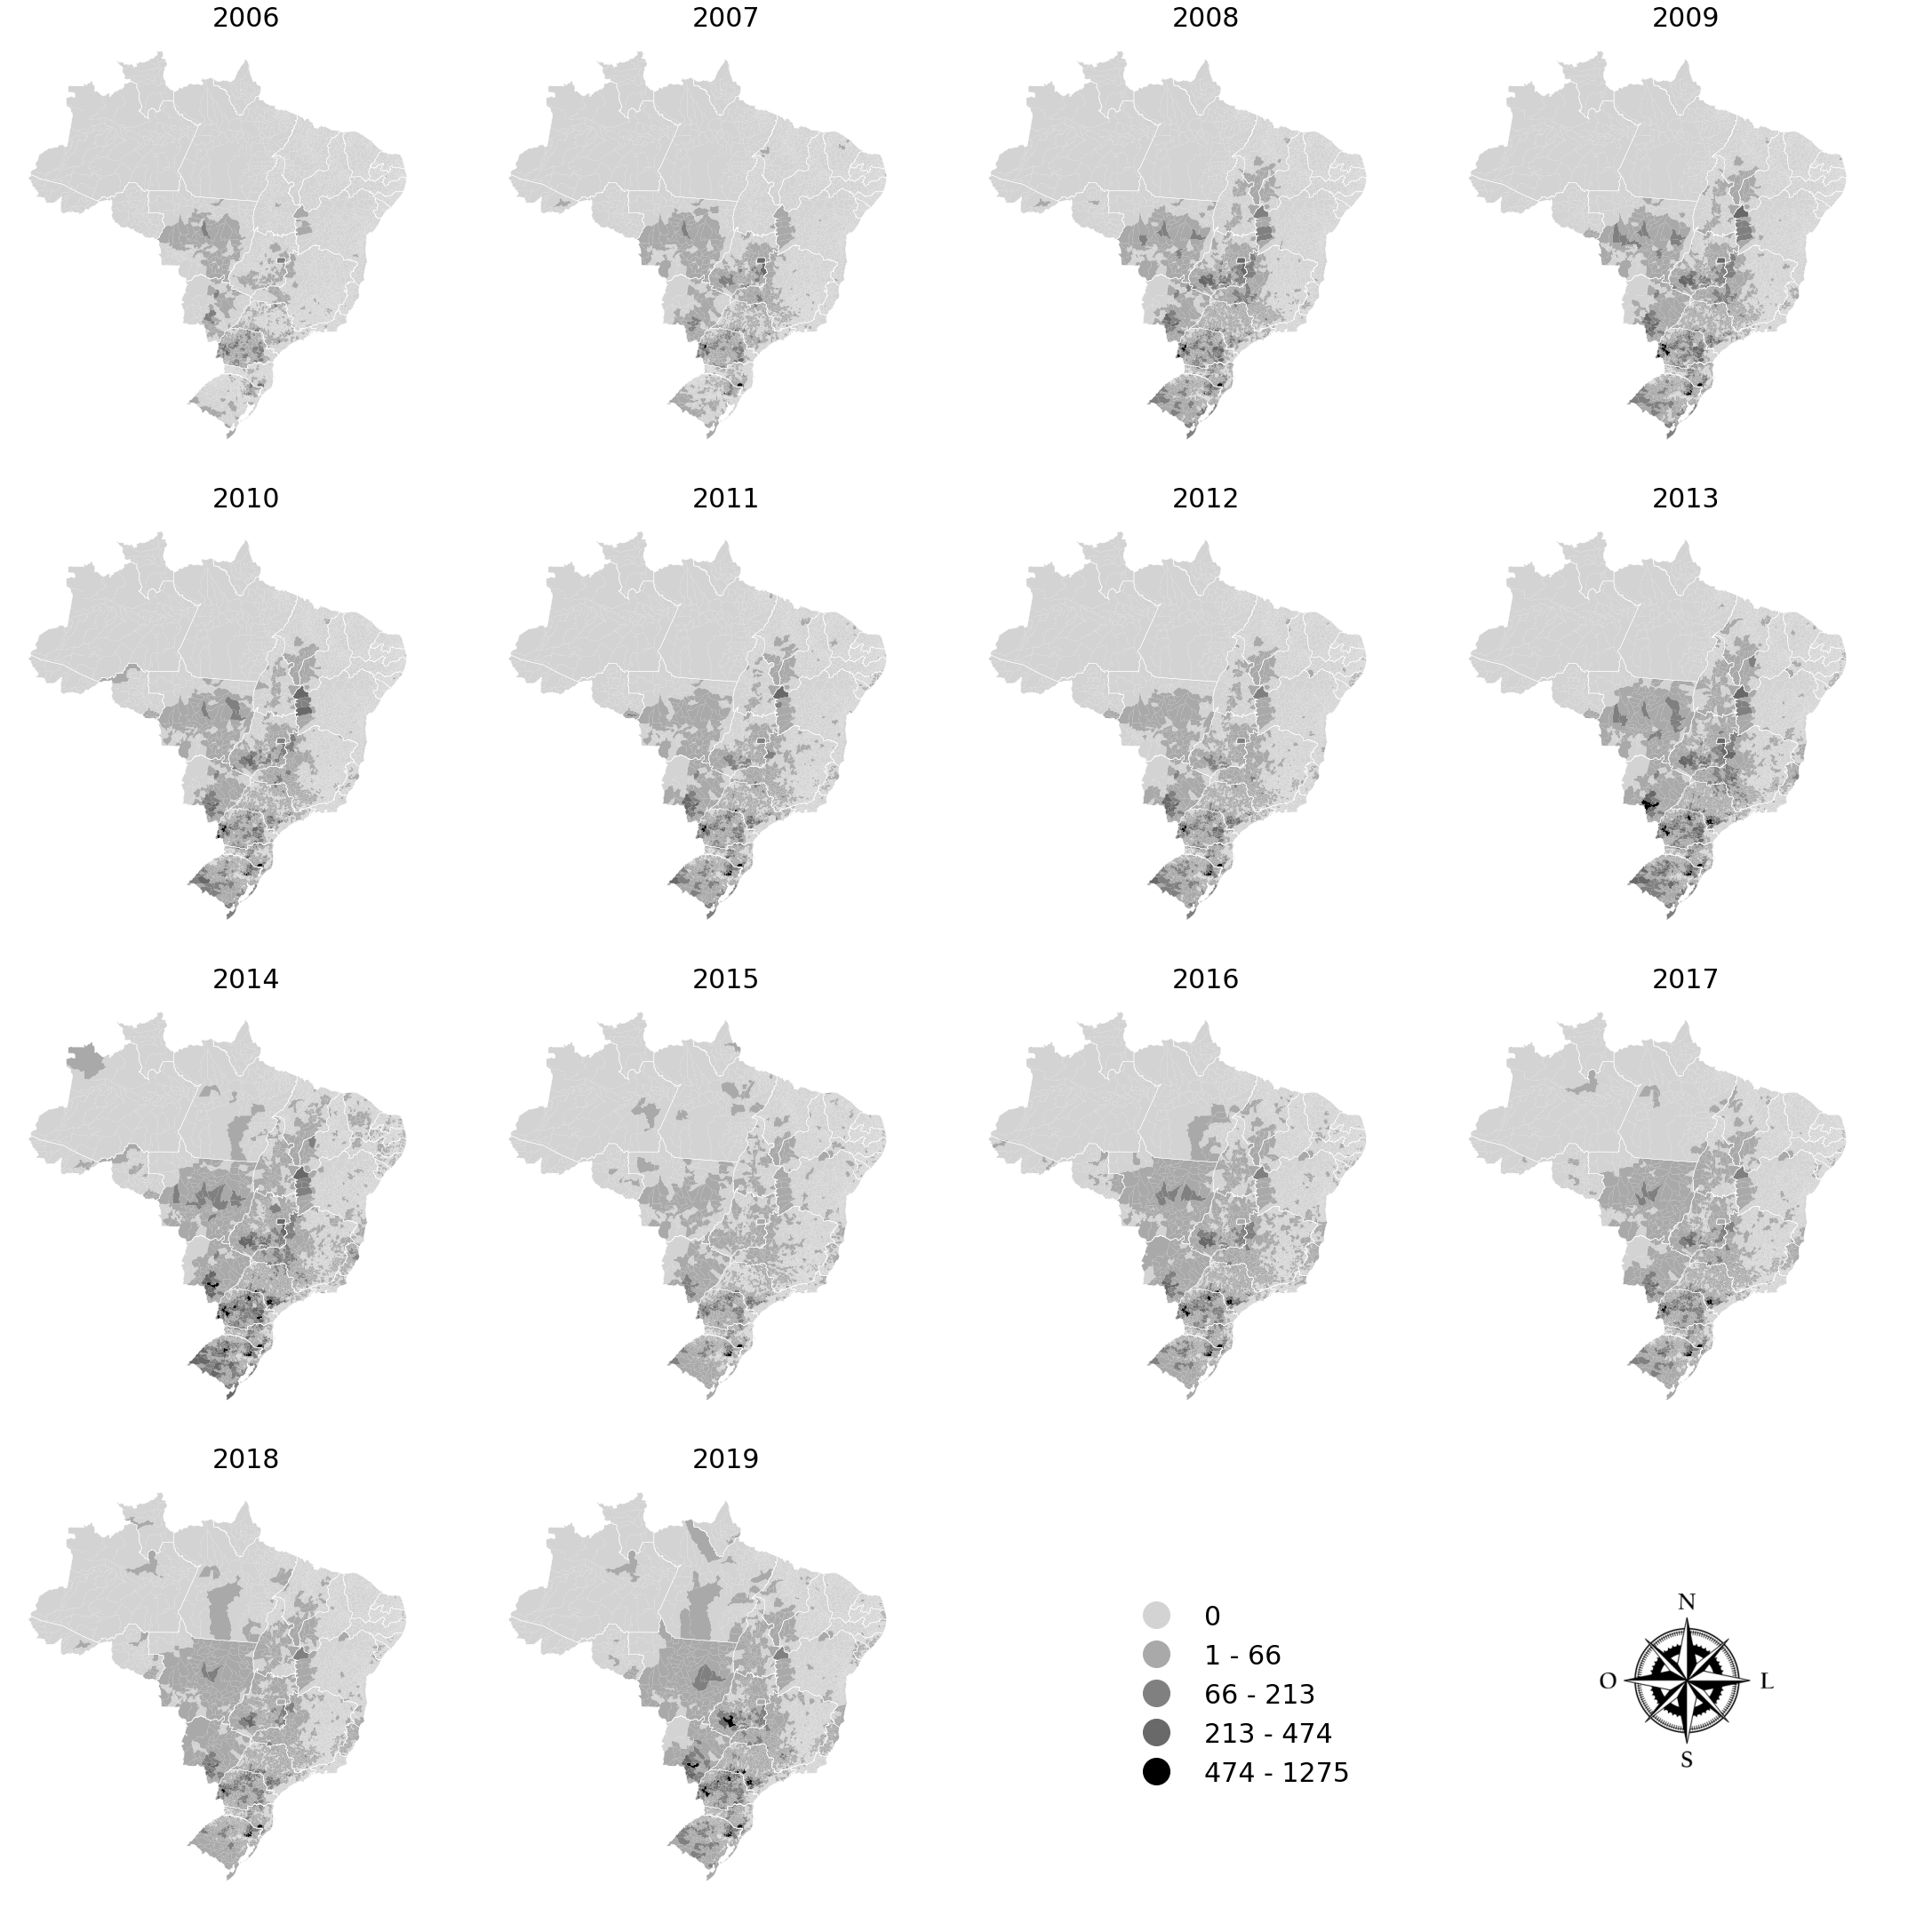
\includegraphics[width=0.9\textwidth]{figuras/map_apolices_contratadas.png}
	\small \textsuperscript {Fonte: Elaboração própria a partir de dados do Ministério da Agricultura, Pecuária e Abastecimento \cite{brasil21b}}
    \label{map_apolices}
\end{figure}

A distribuição espacial das demais variáveis analisadas apresenta um padrão semelhante ao observado com a soma da importância segurada (R\$ milhão)  \footnote{Os mapas da distribuição espacial das variáveis do seguro rural no Brasil são apresentados no apêndice A}. Dessa forma, os resultados corroboram a hipótese apresentada por Silva, Teixeira e Santos (2014) na investigação sobre a participação do PSR na universalização do acesso ao seguro rural. Ou seja, apesar da evolução do seguro rural em âmbito nacional, quando se observa a distribuição espacial, verifica-se que há, ao longo do tempo, uma concentração das apólices e subvenções na região Sul e Centro-Oeste. Portanto, apesar de ter ocorrido uma ampliação do seguro rural, esta ampliação ocorreu de forma concentrada, o que evidencia o cumprimento de forma parcial dos objetivos do PSR \cite{silva14}.

\section{CONSIDERAÇÕES FINAIS}

%O objetivo do presente trabalho foi analisar a evolução e a dinâmica espacial de variáveis do seguro rural nos municípios brasileiros entre 2006 e 2019. Além disso, buscou-se investigar a presença de padrões de distribuição espacial. A

A análise possibilitou constatar resultados positivos na evolução do seguro rural no Brasil. O número de apólices contratadas tem um crescimento de cerca de $8,69$ vezes seu valor inicial durante o período. Ademais, a área agrícola segurada no país praticamente dobrou entre os anos de $2019$ e $2020$, quando alcançou o maior valor, $13,7$ milhões de hectares, que representa $20\%$ da área total agrícola do país. 

Em geral, identificou-se que as maiores concentrações de apólices de seguro rural estão situadas nas regiões Sul, Centro-Oeste e Sudeste, no sul do Estado de São Paulo.  Para mais, ressalta-se que, embora mantenham a concentração do número de apólices contratadas, número de apólices indenizadas, valores de subvenção, indenização e prêmio, atualmente há expansão da demanda por seguros agrícolas. 

Apesar de os dados indicarem uma concentração geográfica da adesão ao sistema de seguro rural no Brasil, é necessário levar em consideração outros sistemas, como o Proagro e o programa Garantia Safra. É necessário, ainda, ressaltar que a adesão dos produtores deve ocorrer como uma resposta à percepção do risco das atividades agropecuárias, ou seja, o seguro deve difundir-se com base na compreensão dos riscos e das vantagens de sua contratação. 

Por fim, este trabalho pode ser entendido como uma abordagem inicial, a partir da qual é possível se introduzir novos métodos estatísticos a fim de aprimorar os resultados. Dentre esses métodos, destaca-se a Análise de Componentes Principais (ACP), que pode ser utilizada para reduzir o número de variáveis,  de forma a possibilitar a incorporação de informação de mais de uma variável na análise exploratória espacial.

\newpage
\addcontentsline{toc}{section}{\hspace*{\distnumber}REFERÊNCIAS}
\begin{center}
\section*{REFERÊNCIAS} 
\end{center}




% Use isso descomentado durante edição.
% Quando concluir a Tese, comente isso e use
% o código do bloco abaixo.
%\begin{singlespace}
%\renewcommand\refname{}
%\begin{flushleft}
%\bibliography{../tese/bibtese2}
%\end{flushleft}
%\end{singlespace}

%% Em cap1intriduc-corrigido.bbl foi feita correção manual de
%% algumas referências como por exemplo as citações
%% de Dissertação e Tese.
%% Então deixa-se de usar o arquivo cap1introduc.bbl gerado
%% automaticamente pelo abntcite, mas isso é só ao final.
\begin{singlespace}
\begin{flushleft}
\renewcommand\refname{}
\vspace*{-1.5cm}
\documentclass[10pt]{article}
%==========================================================================================

\usepackage[utf8]{inputenc}
\usepackage[brazil]{babel}
\usepackage[T1]{fontenc}
\usepackage{amsmath}
\usepackage{amsfonts}
\usepackage{mathrsfs}
\usepackage{amssymb}
\usepackage{graphicx}
\usepackage{geometry, calc, color, setspace}
\usepackage{indentfirst}
\usepackage{wrapfig}
\usepackage{boxedminipage}
\usepackage{enumerate}
\usepackage{float}
\usepackage{paralist}
\usepackage{comment}
\usepackage{icomma}
\usepackage{rotating}
\usepackage{multirow}
\usepackage[position=bottom]{subfig}
\usepackage{array}
\usepackage{tabularx}
\usepackage{float}
\usepackage{array}

\newcolumntype{L}[1]{>{\raggedright\let\newline\\\arraybackslash\hspace{0pt}}m{#1}}
\newcolumntype{C}[1]{>{\centering\let\newline\\\arraybackslash\hspace{0pt}}m{#1}}
%\newcolumntype{R}[1]{>{\raggedleft\let\newline\\\arraybackslash\hspace{0pt}}m{#1}}
\newcolumntype{R}{>{\raggedleft\let\newline\\\arraybackslash\hspace{0pt}}X}

\usepackage[alf,bibjustif]{abntex2cite}
%\usepackage{abntcite}

% Para o alinhamento dos títulos das figuras
\usepackage{caption}
%\captionsetup[figure]{format=hang,labelsep=endash,font=small,justification=RaggedRight,singlelinecheck=off, margin=1cm}
\captionsetup[subfigure]{textfont=small,singlelinecheck=off,justification=raggedright}


%%  Inserindo os códigos Python ==================================
\usepackage{listings}

%\definecolor{light_gray}{rgb}{0.97,0.97,0.97}
%\definecolor{mymauve}{rgb}{0.58,0,0.82}
%\definecolor{mygreen}{rgb}{0,0.6,0}

\lstset{
  language = Python,
  inputencoding = utf8,
  backgroundcolor = \color{white},
  columns=fullflexible,
  basicstyle=\ttfamily,
  breaklines=true,
  postbreak=\raisebox{0ex}[0ex][0ex]{\color{black}$\hookrightarrow$\space},
  keywordstyle=\color{black},      % keyword style
  stringstyle=\color{black},
  commentstyle=\color{black}
}

\newcommand{\HRule}{\noindent\rule{\linewidth}{0.2mm}}

\usepackage{mathpazo}                         % tem suporte matemático
\usepackage[scaled=0.85]{beramono}            % usa esta nos verbatins [scaled=0.9]

\renewcommand\UrlFont{\color{black}\rmfamily} 

\def\distnumber{2.3em}

%==========================================================================================

\author{Walef Machado de Mendonça\footnote{Mestrando em Estatística Aplicada e Biometria na Universidade Federal de Alfenas}\\
Patrícia de Siqueira Ramos\footnote{Professora da Universidade Federal de Alfenas, campus Varginha}}

%==========================================================================================


\title{O seguro rural no Brasil: evolução e distribuição espacial}

\date{}

\begin{document}

\maketitle

\begin{abstract}
As atividades agropecuárias se inserem em um contexto de adversidades que as colocam em situação diferenciada em relação aos riscos enfrentados pelos produtores. Tais atividades demandam grandes investimentos, o que faz com que sua atratividade esteja relacionada às formas existentes de gerenciamento de riscos. Uma das formas mais usuais de gerenciamento de risco neste setor é a contratação de Seguro Rural, uma vez que esta modalidade de seguro possibilita a recuperação da capacidade financeira do produtor na ocorrência de sinistros. Nesse sentido, o objetivo do trabalho é avaliar a distribuição e a dinâmica espacial de variáveis relacionadas às apólices de Seguro Rural contratadas nos municípios brasileiros no período de 2006 a 2019. Além disso, busca-se investigar a existência de dependência espacial e a presença de agrupamentos com grande número de apólices de Seguro Rural. Para tanto, utiliza-se os dados dos Censos do Seguro Rural, compilados pelo Ministério da Agricultura, Pecuária e Abastecimento (MAPA) e Análise Exploratória de Dados Espaciais (AEDE). Os resultados apontam que as maiores concentrações de apólices de Seguro Rural estão situadas nas regiões Sul e Centro-Oeste. Além disso, apesar de haver um aumento nas contratações de Seguro Rural, há também uma tendência de maior concentração espacial das apólices ao longo do período analisado. \\
\newline
\noindent {\textbf{Palavras-chave}}: Seguro rural. Política agrícola. Estatística espacial. Autocorrelação espacial. I de Moran.
\end{abstract}

\section{INTRODUÇÃO}

O setor agropecuário brasileiro tem se destacado nas últimas décadas por seu crescimento proveniente da aplicação de novas tecnologias ao clima tropical e a incorporação de novas áreas de terras \cite{brasil19a}. Segundo dados dos censos agropecuários, entre $2006$ e $2017$, tanto a área total quanto a produção agrícola e pecuária vivenciaram crescimento. Neste período houve um acréscimo de cerca de $5,8\%$ na área total dos estabelecimentos agropecuários \cite{ibge19}. Com relação à sua participação no PIB, em 2019, a parcela do agronegócio brasileiro foi de  $20,5\%$  do PIB nacional. Já em 2020, o setor agropecuário brasileiro alcançou a participação de $26,6\%$ do PIB. Em valores monetários, o PIB do País totalizou R\$ $7,45$ trilhões em 2020, e a participação do agronegócio chegou a quase R\$ $2$ trilhões \cite{cepea21}. 

Dada a relevância do setor agropecuário na economia brasileira, é necessário destacar que este ramo apresenta características muito específicas com relação à magnitude dos riscos aos quais está sujeito \cite{burgo05}. Alguns riscos mais relevantes se devem, principalmente, às instabilidades climáticas e ameaças sanitárias, que podem afetar a produção, ou à razões de mercado, como variações das taxas de câmbio e juros, ou a condições ligadas ao ambiente de negócios, tais como, alterações em marcos regulatórios e em políticas públicas. Todos esses fatores geram variações na renda do setor, que devem ser enfrentadas por meio de políticas de apoio à gestão de riscos \cite{brasil21}. 

Uma gestão de riscos apropriada tem potencial de afetar de forma positiva a estabilidade da renda do produtor e sua própria permanência no setor agropecuário. O gerenciamento de riscos agropecuários pode ocorrer de diversas maneiras, no entanto, a contratação de seguro é uma das medidas mais comuns. O seguro rural é uma importante ferramenta de mitigação de riscos e proteção da renda. Esta modalidade de seguro atua no sentido de amenizar as perdas e possibilitar a recuperação da capacidade financeira do produtor rural em caso de ocorrência de sinistros \cite{brasil19b}. 

Nesse sentido, o presente trabalho tem por objetivo, avaliar a distribuição espacial do seguro rural nos municípios brasileiros entre 2006 e 2019. Para tanto, busca-se investigar se, no Brasil, as variáveis de seguro rural se distribuem de forma aleatória no espaço ou se há padrões de distribuição espacial. Além disso, através da análise da distribuição espacial do seguro rural no período, busca-se identificar se há regiões que tiveram alterações significativas no número de contratações de seguro. Por fim, este estudo busca fornecer informações para o debate de aperfeiçoamentos no sistema de seguro rural brasileiro, de forma a contribuir para uma agricultura mais eficiente e com menores riscos para o produtor rural.

O trabalho está estruturado da seguinte forma: a próxima seção apresenta uma breve revisão de literatura sobre o seguro rural. A terceira seção apresenta os dados, os procedimentos de análise e recursos computacionais que serão utilizados. A quarta seção apresenta resultados e discussões. A última seção apresenta as considerações finais.

\section{UM PANORAMA DO SEGURO RURAL NO BRASIL}

No Brasil, as primeiras iniciativas de se instalar um sistema de seguro rural remontam à meados da década de $1930$ e desenvolveram-se principalmente nas esferas estaduais. Em $1939$, o Estado de São Paulo determinou a criação de um seguro obrigatório contra o granizo na produção de algodão \cite{maia11}. Segundo Silva, Teixeira e Santos (2014), os resultados do seguro para a proteção da lavoura algodoeira em São Paulo influenciaram a criação de novos programas como a Carteira de Seguro Agrícola contra Granizo para a Viticultura, criada em $1948$, e a Carteira de Seguro Agrícola contra Geada para Horticultura instituída em $1964$.

Além disso, Silva, Teixeira e Santos (2014) apontam em seu trabalho o seguro para granizo que foi criado no final da década de $1940$ no Instituto Rio-Grandense do Arroz (Irga), e o seguro criado pela Associação dos Fumicultores do Brasil (Afubra), que objetivava ressarcir com recursos próprios os produtores de fumo nos estados de Santa Catarina e Rio Grande do Sul.

Já no âmbito nacional, foi criado em $1948$, o Instituto de  Resseguros do Brasil (IRB), com o objetivo de reduzir os prejuízos de eventos adversos e assegurar uma maior estabilidade aos produtores rurais \cite{silva14}. Além disso, o Governo Federal criou, em $1954$, a Companhia Nacional de Seguro Agrícola (CNSA) e o Fundo de Estabilidade do Seguro Agrário. Para mais, Maia,  Roitman e de Conti (2011) evidenciaram que a estruturação e gestão dos seguros da CNSA ficaram, de início, sob responsabilidade do IRB. No entanto, segundo Gemignani (2000), as atividades da CNSA se encerraram em $1996$, em decorrência do insucesso em disseminar a adesão ao seguro rural de forma a possibilitar sua viabilidade econômica \cite{maia11, silva14}.

Na segunda metade da década de $1960$, são instituídos o Decreto-Lei nº $73$ ($1966$) e o Decreto nº $60.459$ ($1967$), que instituem os fundamentos institucionais para as atividades de seguro e a criação do Sistema Nacional de Seguros Privados (SNSP). O decreto de $1967$ também criou o Fundo de Estabilidade do Seguro Rural (FESR), cujos recursos inicialmente eram geridos pelo IRB e cujo objetivo principal era garantir a equilíbrio do sistema de seguro rural e fornecer uma cobertura adicional para os riscos de sinistro \cite{silva14}

% Até aqui Ok
Instituída em $1970$, a Resolução nº $5$ do Conselho Nacional de Seguros Privados teve uma função relevante na caracterização das modalidades de seguros agrários. Nesta Resolução, foi definido o seguro agrícola, que fornece cobertura contra perdas decorrentes de fenômenos meteorológicos, doenças e pragas, o seguro pecuário que fornece cobertura para morte de animais causadas por doenças ou acidentes, assim como, o seguro de benfeitorias e produtos agropecuários. Em suma, a Resolução nº $5$ também estabelece o seguro de crédito, que cobre incapacidade de pagamento de compradores dos produtos agropecuários \cite{silva14}.

A criação do Programa de Garantia da Atividade Agropecuária (Proagro), através da Lei nº $5.969$, de $11$ de dezembro de $1973$ ocorreu devido ao fato de que, apesar das diversas ações do Governo Federal, o seguro rural se desenvolveu de forma lenta e restrita à uma pequena parcela da produção \cite{silva14}. O Proagro inicialmente ficou sob a responsabilidade do Banco Central e passou a vincular o seguro rural às operações de crédito agropecuário. Por sua vez, o Banco Central utilizou emissões monetárias para pagamentos de sinistros. Segundo Maia, Roitman e De Conti (2011), o sistema de financiamento do Proagro gerou déficits que provocaram diversas alterações no Programa, que ainda permanece um dos mais importantes instrumentos para a gestão de riscos na agricultura no Brasil.

Instituído por meio da Lei nº $10.823$ de $19$ de dezembro de $2003$ e do Decreto nº $5.121$ de $2004$, o Programa de Subvenção ao Prêmio do Seguro Rural (PSR), passou a ser a política adotada pelo Governo Federal para o estímulo ao sistema de seguro rural no Brasil \cite{brasil18}. O PSR busca, assim como ocorre em países europeus e nos Estados Unidos, conceder subvenção econômica ao valor do prêmio do seguro rural contratado com seguradoras autorizadas \cite{maia11, silva14}.

Dessa forma, o PSR tem como finalidade subsidiar parte do prêmio do seguro rural, de modo a assegurar a responsabilidade do seguro rural como forma de garantir a estabilidade da renda do produtor, além de suscitar o aplicação das tecnologias adequadas para os empreendimentos agropecuários \cite{guia_20}. Tal política do governo busca tornar o seguro rural mais acessível aos agricultores, dividindo os custos de aquisição da apólice entre o governo e os produtores. 


\section{MATERIAL E MÉTODOS}\label{material_e_metodos}

%O objetivo dessa seção é apresentar os dados utilizados no trabalho, descrever a metodologia e os recursos computacionais utilizados na presente análise.

\subsection{DADOS}

% Fonte dos Dados 

Os dados de seguro rural utilizados neste trabalho foram obtidos no endereço eletrônico do Ministério da Agricultura, Pecuária e Abastecimento (MAPA) \cite{brasil21}. Foram utilizados dados com valores anuais a partir do ano de $2006$ até o ano de $2019$ (último ano disponível até então) para os dados municipais. Os dados agregados são provenientes do Atlas do Seguro Rural do MAPA e apresentam periodicidade anual a partir do ano de $2006$. Também foram utilizados dados que contém atributos geográficos, como a posição e o formato, do território brasileiro. Esses dados estão disponíveis no endereço eletrônico do Instituto Brasileiro de Geografia e Estatística \cite{ibge20}.

O conjunto de dados de seguro rural possui informação referente à localização geográfica da contratação do seguro rural. No entanto, foram detectadas algumas divergências relacionadas a distritos ou outras localidades, como fazendas e vilarejos, que foram apontados como o local referente à contratação do seguro. 

Para corrigir essas divergências, de forma a ter informações referentes apenas aos municípios brasileiros, as informações relacionadas às demais localidades foram acrescentadas aos municípios correspondentes. Para a identificação, foi feita uma busca de cada localidade que não tinha correspondência com os municípios brasileiros. Essa busca foi feita inicialmente no site \textit{google maps}, contendo, como termo de busca, o nome da localidade e o seu estado \footnote{Foi considerado que a informação referente aos Estados estava correta nos dados do MAPA}. Nos casos em que a informação do município ao qual a localidade pertencia estava disponível no resultado da pesquisa, o nome do município era utilizado em uma segunda busca no site \textit{Portal Cidades} do IBGE \footnote{\url{https://cidades.ibge.gov.br}}. O \textit{Portal Cidades} apresenta, na maioria dos casos, a divisão territorial e administrativa atualizada, de forma a possibilitar a correção das divergências nos dados. Nos casos em que a informação do município ao qual a localidade pertencia não estava disponível no resultado da pesquisa, o nome da localidade era utilizado como termo de busca de CEPs no site dos Correios \footnote{\url{https://buscacepinter.correios.com.br/app/localidade_logradouro/index.php}}. Para os casos em que não foi possível encontrar nenhum resultado com relação ao município correspondente, a localidade em divergência foi atribuída ao município geograficamente mais próximo \footnote{Os códigos utilizados na análise estão disponíveis no \textit{GitHub} e os link estão no Apêndice B.}.

% Editar essa parte!!!!!
%Variáveis total de apólices contratadas (TAC), soma da importância segurada (R\$ milhão) (SIS), soma dos prêmios (R\$ milhão) (SPR), total de subvenção (R\$ milhão) (TSB), soma das indenizações pagas (R\$ milhão) (SIP), taxa média aplicada às apólices (TMA) e número de apólices indenizadas (NAI).

%\subsection{ANÁLISE DOS DADOS} 

%Após uma análise exploratória dos dados, foi realizada a primeira parte da Análise Exploratória de Dados Espaciais (AEDE), onde os dados agregados por municípios serão apresentados por meio de mapas temáticos, de forma a ilustrar o padrão espacial das variáveis de seguro rural. No segundo passo da AEDE, o valor do \textit{I} de Moram global foi calculado e sua significância obtida por meio do pseudo valor-$p$, obtido a partir de $999$ permutações aleatórias. Neste estudo, foi considerado um nível de significância $\alpha = 0,05$. Foi adotada a matriz de pesos espaciais de contiguidade com a convenção rainha, considerando os vizinhos de primeira ordem. Tal matriz foi adotada por ser a mais utilizada na literatura em trabalhos semelhantes \cite{almeida12}. 

%Para a construção da matriz de pesos espaciais, foram retirados os municípios de Fernando de Noronha, que se constitui em um arquipélago pertencente ao estado de Pernambuco, e Ilhabela, arquipélago no litoral norte do estado de São Paulo. Estes municípios foram desconsiderados pois, além de se constituírem de ilhas, não possuem nenhuma apólice de seguro rural contratada durante os anos em análise. Uma vez definida a matriz, se o valor do \textit{I} de Moran global for significativo, a hipótese de aleatoriedade espacial deve ser rejeitada e há evidências de que há uma autocorrelação positiva \cite{almeida12}. 

%O terceiro passo da análise espacial das variáveis de seguro rural consistiu na obtenção dos mapas \textit{LISA}, de forma a identificar padrões locais de autocorrelação espacial e \textit{outliers} espaciais. Esses mapas ilustram cada uma das observações e indicam se seus valores foram considerados significativos em relação à estatística do I de Moran local \cite{almeida12, anselin95}. 

%\subsection{RECURSOS COMPUTACIONAIS}  

Esse estudo foi feito utilizando a linguagem de programação \textit{Python} \cite{python17}, através da interface \textit{Jupyter} \cite{jupyter17} \cite{perez07} \cite{kluyver19}; Além disso, foram utilizadas as seguintes bibliotecas: \textit{Pandas} \cite{mckinney10}, que é uma ferramenta  para análise e manipulação de dados; \textit{NumPy} \cite{walt11}, que é destinado a possibilitar a computação numérica com \textit{Python}; \textit{SciPy} (JONES et al., 2001); % rever essa citação 
\textit{Matplotlib} \cite{hunter07} e \textit{Seaborn} \cite{waskom14}, que são bibliotecas para criar visualizações  de dados em \textit{Python}; \textit{jenkspy}, para a utilização do algoritmo Fisher Jenks \cite{jenks77} e \textit{Geopandas} \cite{jordahl14}, que possibilita a construção dos mapas. 

\section{RESULTADOS E DISCUSSÃO}

\subsection{A EVOLUÇÃO DO SEGURO RURAL} 

Inicialmente, serão apresentados dados ilustrativos da trajetória do Seguro Rural no Brasil. Serão analisados dados anuais referentes ao número de apólices contratadas, ao número de apólices indenizadas, aos valores de subvenção, indenização e prêmio. Também serão apresentados dados referentes à participação das seguradoras e das principais culturas no número de apólices contratadas. Foram utilizados dados da Plataforma Atlas do Seguro Rural. É importante destacar que os valores referentes ao ano de $2021$ ainda não estavam consolidados na data do presente estudo.

%\subsubsection{Apólices contratadas}

Nesta seção, serão analisados dados anuais referentes às apólices de seguro rural contratadas e os respectivos valores de prêmio e subvenção. 

No gráfico da Figura \ref{apolices_produtores}, é possível observar a evolução do número de produtores e do número de apólices de seguro rural contratadas no período de $2006$ a $2020$. Durante o período analisado, cada produtor contratou, em média, $1,48$ apólices de seguro rural. O número de apólices contratadas tem um crescimento de cerca de $8,69$ vezes durante o período. Entre os anos $2014$ e $2015$, ocorre uma queda de $66,08\%$ nas apólices contratadas. Por sua vez, o número de produtores cresceu $6,36$ vezes entre $2006$ e $2020$.

\begin{figure}[H]
	\centering
	\caption{Número de produtores e apólices de seguro rural contratadas. Brasil $2006 - 2020$}
	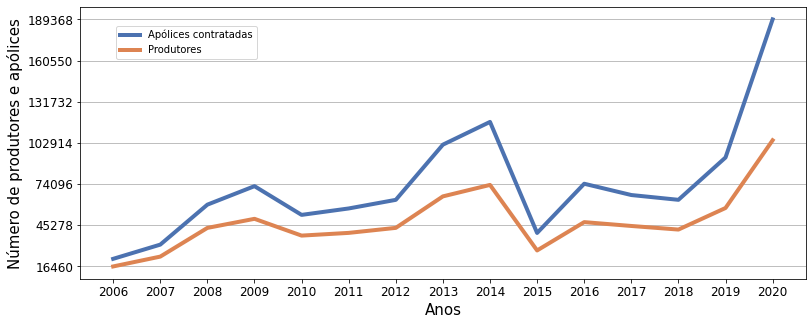
\includegraphics[width=0.8\textwidth]{figuras/apolices_produtores.png}\\
	%\small \textsuperscript {Fonte: Elaboração própria a partir de dados da Plataforma Atlas do Seguro Rural \cite{brasil21b}.}
    \parbox{\dimexpr\linewidth-3cm}{\raggedright
    \strut \textsuperscript{Fonte: Elaboração própria a partir de dados da Plataforma Atlas do Seguro Rural \cite{brasil21b}.}\strut}
    \label{apolices_produtores}
\end{figure}

É importante destacar que, no ano de $2021$, até o mês de junho, havia $66.928$ apólices contratadas \cite{brasil21}. Apesar do valor ser baixo se comparado ao ano de $2020$ ($189.368$ apólices), já é superior a $56,25\%$ dos anos anteriores. Padrão semelhante se observa com o número de produtores. No ano de $2021$, até o mês de junho haviam sido contabilizados $47.472$ produtores segurados \cite{brasil21b}.

%\subsubsection{Valores do prêmio e de subvenção ao prêmio de seguro rural}

O gráfico da Figura \ref{soma_ano_values} apresenta a evolução dos valores em milhões de reais de subvenção ao prêmio de seguro rural, prêmio pago pelo produtor e prêmio recebido pela seguradora entre $2006$ a $2020$. Observa-se que, com exceção do ano de $2014$, é possível notar uma tendência de crescimento dos valores de subvenção e prêmio pagos no período analisado. No ano de 2014, devido à contenções, o governo federal liberou apenas R\$ $400$ milhões dos R\$ $700$ milhões previstos para subsidiar o seguro rural. Esta contenção dos gastos governamentais pode ser um fator a ser considerado na queda dos valores do seguro rural ocorrida entre os anos de $2014$ e $2015$ \cite{andrade21}.

Em $2021$, até o mês de junho, o valor do prêmio pago à seguradora já havia alcançado R\$$1,25$ bilhões, o quarto maior valor registrado e cerca de $50,59\%$ maior que a média. O prêmio do produtor referente ao período de janeiro a junho de $2021$ já era equivalente a R$\$0,77$ bilhões, valor cerca de $69,67\%$ maior que a média do prêmio de responsabilidade do produtor. O valor concedido na forma de subvenção ao prêmio em $2021$ também é o quarto maior valor registrado, cerca de $25,96\%$ maior que a média dos valores de subvenção concedidos . Além disso, a partir do ano de $2016$, a parcela do prêmio sob responsabilidade do produtor passa a superar a parcela concedida pelo governo na forma de subvenção \cite{brasil21b}.

%\begin{figure}[H]
%	\centering
%	\caption{Valores do prêmio e de subvenção ao prêmio de seguro rural. Brasil $2006 - 2020$}
%	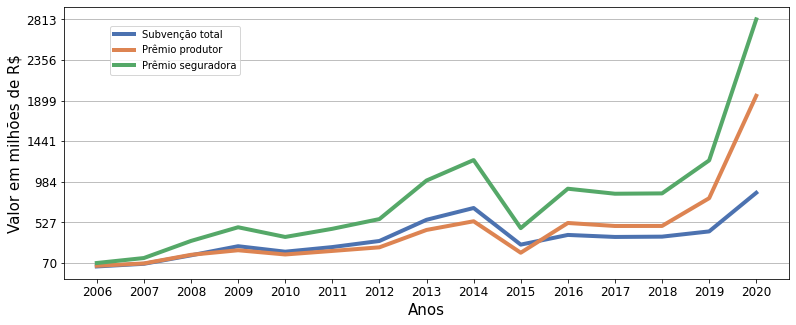
\includegraphics[width=0.8\textwidth]{figuras/soma_ano_values.png}\\
%	\small \textsuperscript {Fonte: Elaboração própria a partir de dados da Plataforma Atlas do Seguro Rural (Mapa, 2021).}
%    \label{soma_ano_values}
%\end{figure}

%\begin{figure}[H]
%	\centering
%	\caption{Soma da importância segurada (R\$ milhões). Brasil $2006 - 2020$}
%	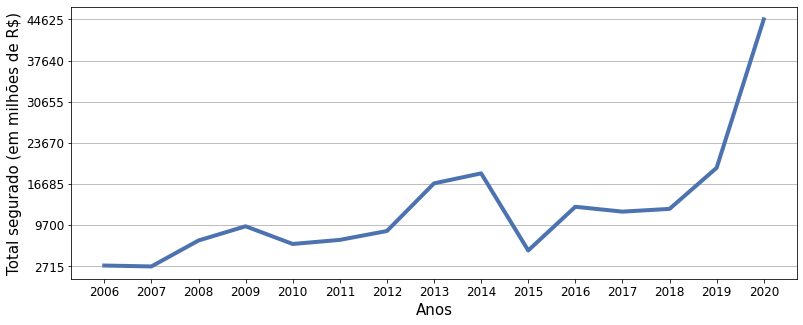
\includegraphics[width=0.8\textwidth]{figuras/total_segurado_mil.png}\\
%	\small \textsuperscript {Fonte: Elaboração própria a partir de dados da Plataforma Atlas do Seguro Rural (Mapa, 2021).}
%    \label{total_segurado_mil}
%\end{figure}

%\begin{figure}[H]
%	\centering
%	\caption{Total da área segurada em hectares. Brasil $2006 - 2020$}
%	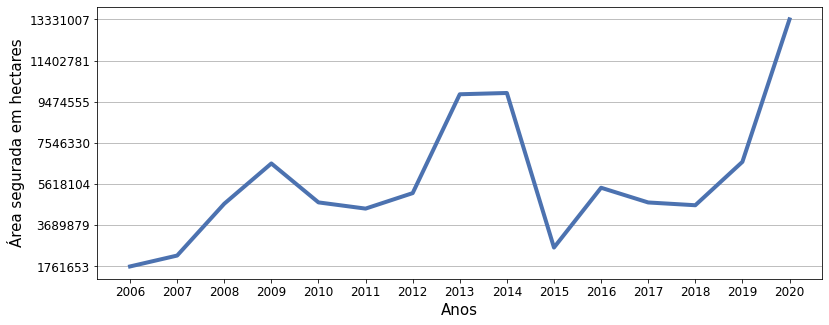
\includegraphics[width=0.8\textwidth]{figuras/area_segurada.png}\\
%	\small \textsuperscript {Fonte: Elaboração própria a partir de dados do Ministério da Agricultura, Pecuária e Abastecimento (MAPA).}
%    \label{area_segurada}
%\end{figure}

%\begin{figure}[H]
%	\centering
%	\caption{Número de apólices de seguro rural indenizadas. Brasil $2006 - 2019$}
%	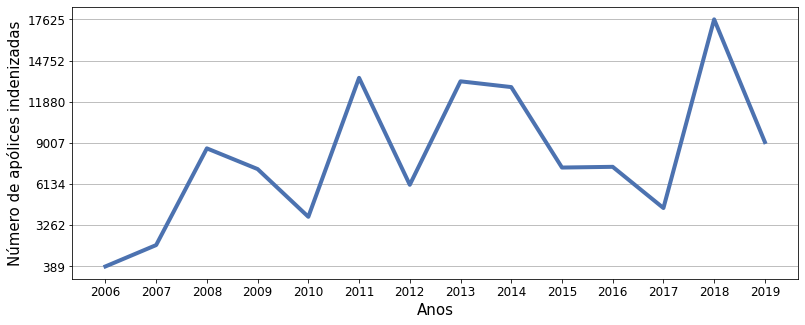
\includegraphics[width=0.8\textwidth]{figuras/apolices_indenizadas.png}\\
%	\small \textsuperscript {Fonte: Elaboração própria a partir de dados do Ministério da Agricultura, Pecuária e Abastecimento (MAPA)}
%    \label{apolices_indenizadas}
%\end{figure}

%\begin{figure}[H]
%	\centering
%	\caption{Valor das indenizações de seguro rural pagas (R\$ milhões). Brasil $2006 - 2019$}
%	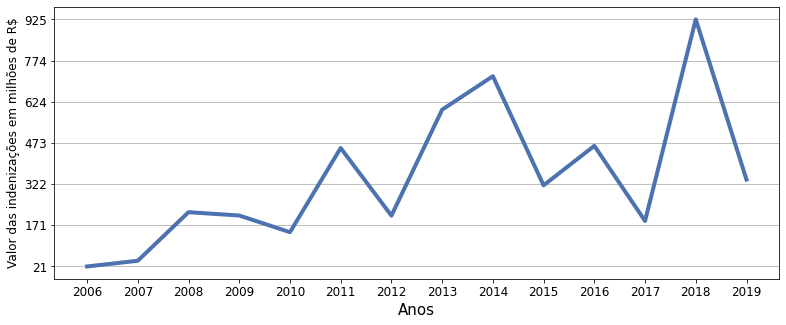
\includegraphics[width=0.8\textwidth]{figuras/valor_indenizacoes.png}\\
%	\small \textsuperscript {Fonte: Elaboração própria a partir de dados do Ministério da Agricultura, Pecuária e Abastecimento (MAPA)}
%    \label{valor_indenizacoes}
%\end{figure}

% variaveis_br
\begin{figure}[H]
	\centering
	\caption{Evolução das variáveis de seguro rural no Brasil}\label{variaveis_br}
	\small
	
	\subfloat[Valores do prêmio e de subvenção ao prêmio de seguro rural\label{soma_ano_values}]{\includegraphics[width=0.45\textwidth]{figuras/soma_ano_values.png}}\hspace{0.1cm}
	\subfloat[Soma da importância segurada (R\$ milhões)\label{total_segurado_mil}]{\includegraphics[width=0.45\textwidth]{figuras/total_segurado_mil.png}}\hspace{0.1cm}\\
	
	\subfloat[Total da área segurada em hectares.\label{area_segurada}]{\includegraphics[width=0.45\textwidth]{figuras/area_segurada.png}}\hspace{0.1cm}
	\subfloat[Número de apólices de seguro rural indenizadas\label{apolices_indenizadas}]{\includegraphics[width=0.45\textwidth]{figuras/apolices_indenizadas.png}}\\
	
	\subfloat[Valor das indenizações de seguro rural pagas (R\$ milhões)\label{valor_indenizacoes}]{\includegraphics[width=0.45\textwidth]{figuras/valor_indenizacoes.png}}\hspace{0.1cm}
	\subfloat[Taxa média anual de contratação do prêmio de seguro rural\label{taxa_media}]{\includegraphics[width=0.45\textwidth]{figuras/taxa_media.png}}
	
	\parbox{\dimexpr\linewidth-2cm}{\raggedright
    \strut \textsuperscript{Fonte: Elaboração própria a partir de dados do Ministério da Agricultura, Pecuária e Abastecimento e da Plataforma
	Atlas do}\strut}\\
    \parbox{\dimexpr\linewidth-2cm}{\raggedright
    \strut \textsuperscript{Seguro Rural \cite{brasil21b}.}\strut}
\end{figure}

Os valores da soma da importância segurada em milhões de reais são apresentados no gráfico da Figura \ref{total_segurado_mil}. Observa-se que há crescimento dos valores segurados, com destaque para o crescimento entre os anos de $2019$ e $2020$, em que o os valores mais que duplicaram. Considerando o período entre $2006$ e $2020$, o crescimento da importância segurada foi de $15,55$ vezes o valor de $2006$. Também é possível observar que, entre os anos de $2014$ e $2015$, ocorreu uma queda de $70,68\%$ do valor segurado.  

Em $2020$, o Programa de Subvenção ao Prêmio do Seguro Rural (PSR) aplicou R\$ $880$ milhões, ou seja, o dobro do valor executado no ano de  $2019$. Para o ano de $2021$, a estimativa apresentada pelo Ministério da Agricultura e Abastecimento foi um aumento de R\$ $1$ bilhão a verba destinada ao PSR \cite{brasil21b}.

No ano de $2014$, o total segurado chegou a R$\$18.462,88$ milhões, no entanto, em $2015$ a soma da importância caiu para R$\$5.398,54$ milhões, o terceiro valor mais baixo do período. O valor mais alto ocorre no ano de $2020$, em que o valor segurado foi de R$\$45,7$ bilhões, o maior desde o início do programa em $2005$.

O valor da importância segurada alcançou $R\$14,4$ bilhões até o mês de junho de $2021$. Este valor é o quinto maior valor da série e já é maior que $25\%$ dos valores registrados nos anos anteriores \cite{brasil21b}. 

%\subsubsection{Área segurada em hectares}

A Figura \ref{area_segurada} apresenta o total da área segurada em hectares nos municípios do Brasil entre os anos de  $2006$ e  $2020$. É possível observar que, a área agrícola segurada no país praticamente dobrou entre $2019$ e $2020$, quando alcançou o maior valor, $13,7$ milhões de hectares, o que representou $20\%$ da área total agrícola do país. O aumento de área em relação a $2019$ é de $98\%$. O maior valor registrado em anos anteriores foi em $2014$, quando foram segurados $9,4$ milhões de hectares. No ano de $2021$, até o mês de junho, foram segurados cerca de $3,76$ milhões de hectares. Esse valor representa cerca de $71,76\%$ da área segurada em $2020$ \cite{brasil21b}. 

%\subsubsection{Indenizações}

Com relação ao número de indenizações,  o gráfico da Figura \ref{apolices_indenizadas} apresenta a evolução das apólices indenizadas ao longo do período analisado. O menor número de indenizações é $389$ em $2006$ e o maior valor ocorreu no ano de $2018$, sendo igual a $17.625$ indenizações. Durante o período, ocorre em média um número de $8.110$ apólices indenizadas por ano, sendo que o crescimento no número de apólices indenizadas foi de $23,31$ vezes entre $2006$ e $2019$. 

Os valores pagos como indenização entre os anos de $2006$ e $2019$ são apresentados no gráfico da Figura \ref{valor_indenizacoes} e variam entre R\$ $20.699.785,74$ em $2006$ e R\$ $924.988.210,45$ em $2018$. A média do valor das indenizações foi de R\$ $345.525.736,50$ no período analisado. 

%\begin{small}
%    \begin{table}[H]
%        \caption{Número de apólices de seguro rural indenizadas por regiões. Brasil $2006-2019$}\label{premio_regioes}
%         \input{../anexos/ap_indeniz_regioes.tex}
%    \end{table}
%\end{small}

%\subsubsection{Taxa média de contratação de seguro rural}

O gráfico apresentado na Figura \ref{taxa_media} mostra a trajetória da taxa de contratação do seguro rural. É possível constatar que a taxa se eleva, em média, de $4,7\%$ em $2006$ para $ 7,46\%$ em $2020$. Até o mês de junho de $2021$, o valor da taxa média havia alcançado $9,79\%$, o segundo maior valor da série, sendo superado pela taxa média cobrada em $2015$, que foi de $10,3\%$ \cite{brasil21b}.  

Segundo Santos e Silva (2017), espera-se que, à medida que o sistema de seguro rural se consolida, reduzam-se os preços das apólices devido aos ganhos de produtividade agropecuária e da redução de fatores de risco. Essas reduções podem ocorrer devido à adoção das orientações do zoneamento agrícola, de um maior conhecimento do histórico de eventos climáticos e dos sinistros ocorridos e, até mesmo em função da adoção de tecnologias, como o uso de irrigação etc. No entanto, essa redução das taxas não ocorreu no período analisado, como observado na Figura \ref{taxa_media}. 

%\begin{figure}[H]
%	\centering
%	\caption{Taxa média anual de contratação do prêmio de seguro rural. Brasil $2006 - 2020$}
%	\includegraphics[width=0.8\textwidth]{figuras/taxa_media.png}\\
%	\small \textsuperscript {Fonte: Elaboração própria a partir de dados da Plataforma Atlas do Seguro Rural (Mapa, 2021).}
%   \label{taxa_media}
%\end{figure}

%\begin{small}
%\begin{table}[H]
%\caption{Taxa média de contratação do prêmio de seguro rural por regiões.  Brasil $2006-2020$}\label{tx_media_regioes}
% \input{../anexos/tx_media_regioes.tex}
%\end{table}
%\end{small}

%\subsubsection{Culturas}

A Figura \ref{percent_cult_apol} apresenta o percentual da participação das maiores culturas no número de apólices de seguro rural contratadas. A análise desse gráfico permite identificar que, com exceção de $2015$, a cultura da soja foi a que mais contratou seguro rural. Além disso, observa-se que o milho 2ª safra \footnote{Nesse caso o milho de 2ª safra é listado em separado devido aos distintos graus de risco em relação à 1ª safra \cite{santos17}.} tem cada vez mais aumentado sua participação no número de apólices contratadas. O milho 1ª safra, por sua vez, tem participação que varia entre $1,23\%$ e $16,46\%$, com média de  $6,16\%$ ao longo do período. A participação da cultura da maçã na contratação de seguro rural permanece relativamente estável ao longo do período, variando entre $8,79\%$ e $14,72\%$. 

\begin{figure}[H]
	\centering
	\caption{Percentual da participação das maiores culturas no número de apólices de seguro rural contratadas. Brasil $2006 - 2019$}
    	\includegraphics[width=0.8\textwidth]{figuras/percent_apolic_cult.png}\\
	%\small \textsuperscript {Fonte: Elaboração própria a partir de dados do Ministério da Agricultura, Pecuária e Abastecimento \cite{brasil21b}}
	\parbox{\dimexpr\linewidth-2.8cm}{\raggedright
    \strut \textsuperscript{Fonte: Elaboração própria a partir de dados do Ministério da Agricultura, Pecuária e Abastecimento \cite{brasil21b}.}\strut}
    \label{percent_cult_apol}
\end{figure}

A Tabela \ref{percent_culturas} apresenta a participação percentual de grupos de culturas em variáveis do seguro rural. É possível constatar que entre os anos de $2006$ e $2020$, as culturas de grãos foram responsáveis por $74,85\%$ das apólices contratadas, seguida das culturas de frutas com $14,74\%$ das apólices no período. Em terceiro lugar está a cultura de olerícolas, com cerca de $3,36\%$ de participação na contratação de apólices de seguro rural. Uma estrutura semelhante de participação percentual de grupos de culturas pode ser observada com relação à participação no valor total segurado. O grupo de cultura que mais se destaca é a dos grãos, com $74,88\%$ do total segurado, seguido das frutas e do café, com $9,55\%$ e $4,04\%$, respectivamente. 

\begin{small}
\begin{table}[H]
\caption{Participação percentual das culturas nos valores do seguro rural. Brasil $2006-2020$}\label{percent_culturas}
 \input{../anexos/percent_culturas.tex}
\end{table}
\end{small}

Além disso, é possível observar na Tabela \ref{percent_culturas}, os percentuais de subvenção ao prêmio de seguro rural e os valores da taxa média de contratação do seguro. As taxas cobradas durante o período para a cultura de grãos foi de $7,70\%$, a taxa cobrada das culturas de frutas foi de $9,17\%$ e as olerícolas tiveram uma taxa média de contratação de $7,64\%$. Os percentuais de subvenção dessas culturas são, também, os mais altos: $77,35\%$ de subvenção para os grãos, $16,07\%$ para as culturas de frutas e $2,85\%$ para as olerícolas. Ou seja, os grupos de culturas com maior demanda pelo seguro, além de apresentarem os maiores valores de apólices, os maiores valores e maior ocorrência de sinistros, são também aqueles com maiores taxas médias. 

De acordo com  Santos e Silva (2017), este fato pode apontar para a possibilidade de dois fenômenos a serem melhor examinados. O primeiro diz respeito à situação em que as maiores taxas resultam do fato de que maiores subvenções são dadas a cultivos de maior risco. O segundo fenômeno possível é que as taxas sejam mais altas, principalmente no caso dos produtores que adotam o ZARC, com elevada tecnologia produtiva, alta produtividade e não têm estas características levadas em consideração como informação que contribui para a redução das taxas. Dessa forma, se por um lado o seguro agrícola não se consolida sem a subvenção dada pelo Estado, por outro, é possível que esse sistema de subvenção ao prêmio crie distorções no mercado de seguro rural. 

%\subsubsection{Seguradoras}

A Tabela \ref{seguradoras} exibe a distribuição das fatias de mercado das seguradoras entre $2006$ e $2020$. Apesar de as seguradoras passarem de cinco, em $2006$, para $16$ companhias aptas a operar com seguro rural em $2020$, é possível constatar que há uma concentração do mercado de seguro em um número reduzido de seguradoras. 

\begin{small}
\begin{table}[H]
\caption{Participação de mercado das seguradoras. Brasil $2006-2020$}\label{seguradoras}
 \input{../anexos/produtores_seg.tex}
\end{table}
\end{small}

Ao se analisar a participação no percentual do número de apólices de seguro rural, percebe-se que apenas as três maiores seguradoras (Brasilseg, Mapfre e Essor) concentram cerca de $61,56\%$ do mercado. Com relação ao percentual dos beneficiários, as três maiores seguradoras contam com cerca de $51,60\%$ dos beneficiários durante o período analisado. A concentração é ainda maior quando se analisa o percentual da área segurada, sendo que a  maior seguradora do ramo (Brasilseg) conta com um percentual de $55,31\%$ da área segurada em hectares. As três maiores seguradoras são responsáveis pelo seguro de $72,78\%$ da área segurada. 

%A próxima seção tem como objetivo apresentar os resultados da análise da distribuição espacial dos dados do seguro rural no Brasil. 

\subsection{A DISTRIBUIÇÃO REGIONAL DO SEGURO RURAL} 

Os gráficos apresentados na Figura \ref{variaveis_regioes} exibem a evolução, entre os anos de $2006$ e $2019$, das variáveis de seguro rural analisadas por regiões.

Na figura \ref{ap_contrat_regioes}, é possível observar a evolução do número de apólices contratadas nas regiões brasileiras. Na Figura \ref{ap_contrat_regioes}, observa-se que a região Sul se destaca das demais com relação ao número de apólices contratadas. O menor número de apólices contratadas na região Sul foi de $16.525$ apólices no ano de $2006$. O valor médio de apólices contratadas durante o período foi $44.166$ apólice. No ano de $2014$, foi registrado o maior número de apólices contratadas ($76.668$ apólices). 

% variaveis_regioes
\begin{figure}[H]
	\centering
	\caption{Evolução das variáveis de seguro rural por regiões. Brasil $2006 - 2019$}\label{variaveis_regioes}
	\small
	
	\subfloat[Número de apólices contratadas\label{ap_contrat_regioes}]{\includegraphics[width=0.45\textwidth]{figuras/ap_contrat_regioes.png}}\hspace{0.1cm}
	\subfloat[Total segurado (em milhões de R\$)\label{t_segurado_regioes}]{\includegraphics[width=0.45\textwidth]{figuras/t_segurado_regioes.png}}\\
	
	\subfloat[Valores de prêmio (em milhões de R\$)\label{soma_premio_regioes}]{\includegraphics[width=0.45\textwidth]{figuras/soma_premio_regioes.png}}\hspace{0.1cm}
	\subfloat[Valores subvenção (em milhões de R\$)\label{t_subvencao_regioes}]{\includegraphics[width=0.45\textwidth]{figuras/t_subvencao_regioes.png}}\\
	
	\subfloat[Apólices indenizadas\label{ap_indeniz_regioes}]{\includegraphics[width=0.45\textwidth]{figuras/ap_indeniz_regioes.png}}\hspace{0.1cm}
	\subfloat[Valor das indenizações (em milhões de R\$)\label{inde_pagas_regioes}]{\includegraphics[width=0.45\textwidth]{figuras/inde_pagas_regioes.png}}\\
	
    \parbox{\dimexpr\linewidth-2cm}{\raggedright
    \strut \textsuperscript{Fonte: Elaboração própria a partir de dados do Ministério da Agricultura, Pecuária e Abastecimento \cite{brasil21b}}\strut}
\end{figure}

A segunda região com maior número de apólices contratadas é a região Sudeste (Figura \ref{ap_contrat_regioes}). Em média, na região Sudeste, foram contratadas $12.942$ apólices por ano, o maior valor registrado foi $26.913$ apólices contratadas em $2013$. A região Centro-Oeste é a terceira região com mais apólices contratadas, sendo que em média foram contratadas $7.225$  por ano e, em $2013$ foi registrado o maior número de apólices ($12.260$). Por fim, as regiões Norte e Nordeste, apresentaram respectivamente, em média, $240$ e $804$ apólices contratadas por ano.

A taxa de crescimento do número de apólices contratadas na região sul foi de $3,72$ vezes o valor inicial entre os anos $2006$ e $2019$. Por sua vez, durante o período analisado a região Sudeste teve um crescimento do número apólices de $5,87$ vezes e a região Centro-Oeste apresentou um crescimento do número de apólices de $6,66$ vezes. As regiões Norte e Nordeste apresentaram um crescimento médio anual igual a $0,14\%$ e $4,04\%$ respectivamente. 

Ao se analisar a evolução do total segurado nas regiões brasileiras apresentado na Figura \ref{t_segurado_regioes}, é possível observar que a região Sul se destaca com, em média, $5146,83$ milhões de valor segurado total. O maior valor foi registrado em $2019$ e foi igual a $9520,85$ milhões, o segundo maior valor foi igual a $8664,31$ milhões e foi registrado em $2015$. 

No início da série valores a região Centro-Oeste apresenta um maior valor total segurado do que a região Sul (5.355 milhões). Além disso, como é possível observar na Figura \ref{t_segurado_regioes}, a partir do ano de $2016$ a região Centro-Oeste supera a região Sudeste no valor total segurado. A região Norte apresentou, com relação ao total segurado, os valores de $120,35$ milhões em $2009$ e $197,01$ milhões em $2014$. 
Além disso, a região Norte apresenta o seu maior valor no ano de $2019$, com total segurado igual a $509,94$ milhões. Também é possível observar que há indícios de haver um crescimento do total segurado em todas as regiões. 

O total segurado na região Sul apresenta um crescimento de cerca de $10,27$ vezes entre os anos de $2006$ e $2019$. Na região Sudeste, o crescimento foi de $22,52$ vezes o valor registrado em $2006$. Por sua vez, o Centro-Oeste apresentou um crescimento de cerca de $3,07$ vezes o valor do total segurado durante o período. O valor do total segurado na região Norte cresceu $499.51$ vezes entre os anos $2006$ e $2019$. Por fim, no Nordeste, o valor total segurado apresentou um crescimento de $106,95$ vezes o valor inicial. 

Para mais, ao se analisar a Figura \ref{soma_premio_regioes} e \ref{t_subvencao_regioes}, é possível observar que as variáveis valores de prêmio e valores subvenção apresentam crescimento durante o período analisado. Também é possível observar que, com exceção das variáveis relacionadas à indenização, as variáveis apresentam uma queda entre os anos de $2014$ e $2015$.

É possível observar na Figura \ref{ap_indeniz_regioes}, que a região Sul se destaca quando se analisa o número de apólices indenizadas. Os valores variam de $237$ em $2006$ e $13812$ apólices indenizadas em $2019$. Em média, a região Sul teve cerca de $6364$ apólices indenizadas durante o período. Além disso, durante os anos analisados, houve um crescimento de $58,28\%$ no número de apólices de seguro rural indenizadas. A região Sudeste é a segunda região com maior número de apólices indenizadas, sendo que o menor número de apólices indenizadas na região Sudeste foi de $135$ e ocorreu em $2006$, com maior valor registrado em $2013$, equivalente a $2.616$. 

Ao longo dos anos analisados, a diferença entre o número de apólices na região Sul e Sudeste foi em média igual a $5.283$ apólices. A região Centro-Oeste foi responsável por, em média, $559,64$ apólices indenizadas. O maior número de apólices indenizadas na região Centro-Oeste foi registrado em $2018$ e foi igual a $1561$ apólices. As regiões Norte e Nordeste tiveram em média $15,57$ e $88,64$, respectivamente. 

Com relação ao valor das indenizações de seguro rural pagas, é possível observar na Figura \ref{inde_pagas_regioes}, que a região Sul é a que possui os maiores valores pagos como indenização. Em média, foram pagos R$\$205,66$ milhões como indenização. O maior valor foi equivalente a R$\$551,74$ milhões e foi registrado em $2018$ e o menor valor foi registrado no primeiro ano analisado, sendo equivalente a R$\$15.06$ milhões. 

A Tabela \ref{media_regioes} apresenta a média dos valores anuais das variáveis de seguro rural acumulados por regiões no Brasil no período de $2006$ e $2019$. Como é possível observar, que a região Sul se destaca das demais com os maiores valores das médias das variáveis. Com relação ao número de apólices contratadas, a segunda região com maior média da variável total de apólices contratadas é o Sudeste. No entanto, quando se analisa a média da soma da importância seguradas, a segunda região com maior média é a região Centro-Oeste. A região Centro-Oeste, também conta com maiores médias nas variáveis soma dos prêmios pagos, total da subvenção e soma das indenizações pagas com relação às regiões Norte, Nordeste e Sudeste. A região Sudeste apresenta a maior média anual do número de apólices indenizadas. 



\begin{small}
\begin{table}[H]
\caption{Média anual dos valores das variáveis de seguro rural por regiões. Brasil $2006-2019$}\label{media_regioes}
\input{../anexos/media_regioes.tex}
\end{table}
\end{small}

A média dos valores anuais da taxa média de contratação de apólices indica que, a região Sul é a que possui maior taxa de contratação de seguro com taxa média igual a $0,45$ ao longo dos anos. A região Centro-Oeste é a que tem o segundo maior valor de taxa média durante os anos, sendo igual a $0,13$. As regiões Norte e Nordeste apresentaram taxa média igual a $0,01$.

\subsection{DISTRIBUIÇÃO ESPACIAL DO SEGURO RURAL}

A análise da distribuição espacial das variáveis se inicia com a visualização dos mapas temáticos. Por meio destes mapas, busca-se identificar visualmente se há a ocorrência de padrões na distribuição espacial das variáveis do seguro rural.

O primeiro grupo de mapas, apresentado na Figura \ref{map_segurado}, exibe a distribuição espacial da soma da importância segurada (R\$ milhão) nos municípios brasileiros entre os anos de $2006$ e $2019$. Para a construção dos mapas, os valores da variável foram divididos em 5 intervalos \footnote{Para a criação dos intervalos foi aplicado algoritmo Fisher Jenks aos valores das variáveis diferentes de $0$ e os intervalos foram criados tendo como referência os valores do ano de 2019 \cite{jenks77}}.

\begin{figure}[H]
	\centering
	\caption{Total segurado por municípios (em mil R\$). Brasil $2006 - 2019$}
	\includegraphics[width=0.9\textwidth]{figuras/map_total_segurado_mil.png}
	\small \textsuperscript {Fonte: Elaboração própria a partir de dados do Ministério da Agricultura, Pecuária e Abastecimento \cite{brasil21b}}
    \label{map_segurado}
\end{figure}

Pela análise da Figura \ref{map_segurado}, é possível observar que a distribuição espacial do total segurado se modificou no decorrer dos anos, apesar de se concentrar principalmente nas Regiões Sul e Centro-Oeste. É possível também destacar que, durante o período analisado, há indícios de concentrações espaciais na região do Extremo Oeste Baiano no Estado da Bahia, Sudoeste de Mato Grosso do Sul, Sul Goiano no Estado de Goiás e Sudeste, no sul do Estado de São Paulo.

O conjunto de mapas apresentado na Figura \ref{map_apolices}, exibe o número de apólices de seguro rural contratadas por municípios entre $2006$ e $2019$. Ao longo dos anos, o número de municípios com nenhuma apólice contratada cai e há indícios de um aumento do número de apólices até o ano de $2014$. Entre os anos de $2014$ e $2015$, há uma queda no número de apólices contratadas, como já foi mostrado no gráfico da Figura \ref{apolices_produtores}, e das demais variáveis relacionadas ao seguro rural. Essa redução também pode ser visualizada no mapa da Figura \ref{map_apolices}, em que o ano de $2015$ apresenta municípios com menor número de apólices contratadas. 

Ao se analisar a distribuição espacial, observa-se que há indícios de haver uma maior concentração espacial do total segurado e do número de apólices de seguro rural contratadas em algumas regiões. A partir do ano de $2015$ a retomada do crescimento destas variáveis (Figura \ref{total_segurado_mil}) pode ser visualizado com um maior número de áreas de coloração mais escura nos mapas (Figuras \ref{map_segurado} e \ref{map_apolices}).

\begin{figure}[H]
	\centering
	\caption{Número de apólices de seguro rural contratadas por municípios. Brasil $2006 - 2019$}
	\includegraphics[width=0.9\textwidth]{figuras/map_apolices_contratadas.png}
	\small \textsuperscript {Fonte: Elaboração própria a partir de dados do Ministério da Agricultura, Pecuária e Abastecimento \cite{brasil21b}}
    \label{map_apolices}
\end{figure}

A distribuição espacial das demais variáveis analisadas apresenta um padrão semelhante ao observado com a soma da importância segurada (R\$ milhão)  \footnote{Os mapas da distribuição espacial das variáveis do seguro rural no Brasil são apresentados no apêndice A}. Dessa forma, os resultados corroboram a hipótese apresentada por Silva, Teixeira e Santos (2014) na investigação sobre a participação do PSR na universalização do acesso ao seguro rural. Ou seja, apesar da evolução do seguro rural em âmbito nacional, quando se observa a distribuição espacial, verifica-se que há, ao longo do tempo, uma concentração das apólices e subvenções na região Sul e Centro-Oeste. Portanto, apesar de ter ocorrido uma ampliação do seguro rural, esta ampliação ocorreu de forma concentrada, o que evidencia o cumprimento de forma parcial dos objetivos do PSR \cite{silva14}.

\section{CONSIDERAÇÕES FINAIS}

%O objetivo do presente trabalho foi analisar a evolução e a dinâmica espacial de variáveis do seguro rural nos municípios brasileiros entre 2006 e 2019. Além disso, buscou-se investigar a presença de padrões de distribuição espacial. A

A análise possibilitou constatar resultados positivos na evolução do seguro rural no Brasil. O número de apólices contratadas tem um crescimento de cerca de $8,69$ vezes seu valor inicial durante o período. Ademais, a área agrícola segurada no país praticamente dobrou entre os anos de $2019$ e $2020$, quando alcançou o maior valor, $13,7$ milhões de hectares, que representa $20\%$ da área total agrícola do país. 

Em geral, identificou-se que as maiores concentrações de apólices de seguro rural estão situadas nas regiões Sul, Centro-Oeste e Sudeste, no sul do Estado de São Paulo.  Para mais, ressalta-se que, embora mantenham a concentração do número de apólices contratadas, número de apólices indenizadas, valores de subvenção, indenização e prêmio, atualmente há expansão da demanda por seguros agrícolas. 

Apesar de os dados indicarem uma concentração geográfica da adesão ao sistema de seguro rural no Brasil, é necessário levar em consideração outros sistemas, como o Proagro e o programa Garantia Safra. É necessário, ainda, ressaltar que a adesão dos produtores deve ocorrer como uma resposta à percepção do risco das atividades agropecuárias, ou seja, o seguro deve difundir-se com base na compreensão dos riscos e das vantagens de sua contratação. 

Por fim, este trabalho pode ser entendido como uma abordagem inicial, a partir da qual é possível se introduzir novos métodos estatísticos a fim de aprimorar os resultados. Dentre esses métodos, destaca-se a Análise de Componentes Principais (ACP), que pode ser utilizada para reduzir o número de variáveis,  de forma a possibilitar a incorporação de informação de mais de uma variável na análise exploratória espacial.

\newpage
\addcontentsline{toc}{section}{\hspace*{\distnumber}REFERÊNCIAS}
\begin{center}
\section*{REFERÊNCIAS} 
\end{center}




% Use isso descomentado durante edição.
% Quando concluir a Tese, comente isso e use
% o código do bloco abaixo.
%\begin{singlespace}
%\renewcommand\refname{}
%\begin{flushleft}
%\bibliography{../tese/bibtese2}
%\end{flushleft}
%\end{singlespace}

%% Em cap1intriduc-corrigido.bbl foi feita correção manual de
%% algumas referências como por exemplo as citações
%% de Dissertação e Tese.
%% Então deixa-se de usar o arquivo cap1introduc.bbl gerado
%% automaticamente pelo abntcite, mas isso é só ao final.
\begin{singlespace}
\begin{flushleft}
\renewcommand\refname{}
\vspace*{-1.5cm}
\documentclass[10pt]{article}
\input{../tese/preambulosimples.tex}

\title{O seguro rural no Brasil: evolução e distribuição espacial}

\date{}

\begin{document}

\maketitle

\begin{abstract}
\input{cap1resumo.tex}
\end{abstract}

\input{cap1.tex}

% Use isso descomentado durante edição.
% Quando concluir a Tese, comente isso e use
% o código do bloco abaixo.
%\begin{singlespace}
%\renewcommand\refname{}
%\begin{flushleft}
%\bibliography{../tese/bibtese2}
%\end{flushleft}
%\end{singlespace}

%% Em cap1intriduc-corrigido.bbl foi feita correção manual de
%% algumas referências como por exemplo as citações
%% de Dissertação e Tese.
%% Então deixa-se de usar o arquivo cap1introduc.bbl gerado
%% automaticamente pelo abntcite, mas isso é só ao final.
\begin{singlespace}
\begin{flushleft}
\renewcommand\refname{}
\vspace*{-1.5cm}
\input{cap1introduc.bbl}
\end{flushleft}
\end{singlespace}

%%.....................................................
%% inclui anexos

\newpage
\addcontentsline{toc}{section}{\hspace*{\distnumber}APÊNDICES}
\begin{center}
\section*{APÊNDICES} 
\end{center}

\begin{singlespace}
\noindent{{APÊNDICE A -- } Mapas da distribuição espacial das variáveis do seguro rural no Brasil, de 2006 a 2019}
\end{singlespace}
\noindent
\begin{small}
\linespread{0.86}
\input{../anexos/anexo_mapa_tematico.txt}
\end{small}

\newpage
\begin{singlespace}
\noindent{{APÊNDICE B -- } Mapas \textit{LISA} das variáveis do seguro rural no Brasil, de 2006 a 2019}
\end{singlespace}
\noindent
\begin{small}
\linespread{0.86}
\input{../anexos/anexo_mapa_lisa.txt}
\end{small}

\newpage
\begin{singlespace}
\noindent{{APÊNDICE C -- } Código em Python reproduzível correspondente ao tratamento dos dados.}
\end{singlespace}
\noindent
\vspace{0.5cm}
%\noindent \rule[4mm]{\textwidth}{0.1ex}
\begin{small}
\linespread{0.7}
\vspace{-1cm}
\input{scripts/SR_DATA.py} 
\noindent \rule[4mm]{\textwidth}{0.1ex}
\end{small}

\end{document}

%==========================================================================================

\end{flushleft}
\end{singlespace}

%%.....................................................
%% inclui anexos

\newpage
\addcontentsline{toc}{section}{\hspace*{\distnumber}APÊNDICES}
\begin{center}
\section*{APÊNDICES} 
\end{center}

\begin{singlespace}
\noindent{{APÊNDICE A -- } Mapas da distribuição espacial das variáveis do seguro rural no Brasil, de 2006 a 2019}
\end{singlespace}
\noindent
\begin{small}
\linespread{0.86}
%\begin{figure}[H]
%	\centering
%	\caption{Apólices de seguro rural contratadas por municípios brasileiros, de 2006 a 2019}
%	\includegraphics[width=0.9\textwidth]{figuras/map_apolices_contratadas.png}\\
%	\small \textsuperscript {Fonte: Elaboração própria a partir de dados do Ministério da Agricultura, Pecuária e Abastecimento (MAPA)}
%    \label{map_apolices}
%\end{figure}

\begin{figure}[H]
	\centering
	\caption{Apólices de seguro rural indenizadas por municípios brasileiros, de 2006 a 2019}
	\includegraphics[width=0.9\textwidth]{figuras/map_apolices_indenizadas.png}
	\small \textsuperscript {Fonte: Elaboração própria a partir de dados do Ministério da Agricultura, Pecuária e Abastecimento (MAPA)}
    \label{map_lisa_indenizadas}
\end{figure}

%\begin{figure}[H]
%	\centering
%	\caption{Sinistralidade média do seguro rural contratadas por municípios brasileiros, de 2006 a 2019}
%	\includegraphics[width=0.9\textwidth]{figuras/map_sinistralidade_media.png}
%	\small \textsuperscript {Fonte: Elaboração própria a partir de dados do Ministério da Agricultura, Pecuária e Abastecimento (MAPA)}
%    \label{map_lisa_sinistralidade}
%\end{figure}

\begin{figure}[H]
	\centering
	\caption{Soma dos prêmios de seguro rural por municípios brasileiros, de 2006 a 2019 (em mil R\$)}
	\includegraphics[width=0.9\textwidth]{figuras/map_soma_premio_total_mil.png}
	\small \textsuperscript {Fonte: Elaboração própria a partir de dados do Ministério da Agricultura, Pecuária e Abastecimento (MAPA)}
    \label{map_lisa_soma_premio}
\end{figure}

\begin{figure}[H]
	\centering
	\caption{Taxa média das apólices de seguro rural contratadas por municípios brasileiros, de 2006 a 2019}
	\includegraphics[width=0.9\textwidth]{figuras/map_taxa_media.png}
	\small \textsuperscript {Fonte: Elaboração própria a partir de dados do Ministério da Agricultura, Pecuária e Abastecimento (MAPA)}
    \label{map_lisa_taxa_media}
\end{figure}

\begin{figure}[H]
	\centering
	\caption{Total da subvenção ao prêmio de seguro rural (em mil R\$) por municípios brasileiros, de 2006 a 2019}
	\includegraphics[width=0.9\textwidth]{figuras/map_total_subvencao_mil.png}
	\small \textsuperscript {Fonte: Elaboração própria a partir de dados do Ministério da Agricultura, Pecuária e Abastecimento (MAPA)}
    \label{map_lisa_subvencao}
\end{figure}

\begin{figure}[H]
	\centering
	\caption{Valor das indenizações de seguro rural pagas por municípios brasileiros, de 2006 a 2019 (em mil R\$)}
	\includegraphics[width=0.9\textwidth]{figuras/map_indenizacoes_pagas_mil.png}
	\small \textsuperscript {Fonte: Elaboração própria a partir de dados do Ministério da Agricultura, Pecuária e Abastecimento (MAPA)}
    \label{map_lisa_indenizacoes}
\end{figure}



\end{small}

\newpage
\begin{singlespace}
\noindent{{APÊNDICE B -- } Mapas \textit{LISA} das variáveis do seguro rural no Brasil, de 2006 a 2019}
\end{singlespace}
\noindent
\begin{small}
\linespread{0.86}
\input{../anexos/anexo_mapa_lisa.txt}
\end{small}

\newpage
\begin{singlespace}
\noindent{{APÊNDICE C -- } Código em Python reproduzível correspondente ao tratamento dos dados.}
\end{singlespace}
\noindent
\vspace{0.5cm}
%\noindent \rule[4mm]{\textwidth}{0.1ex}
\begin{small}
\linespread{0.7}
\vspace{-1cm}
\input{scripts/SR_DATA.py} 
\noindent \rule[4mm]{\textwidth}{0.1ex}
\end{small}

\end{document}

%==========================================================================================

\end{flushleft}
\end{singlespace}

%%.....................................................
%% inclui anexos

\newpage
\addcontentsline{toc}{section}{\hspace*{\distnumber}APÊNDICES}
\begin{center}
\section*{APÊNDICES} 
\end{center}

\begin{singlespace}
\noindent{{APÊNDICE A -- } Mapas da distribuição espacial das variáveis do seguro rural no Brasil, de 2006 a 2019}
\end{singlespace}
\noindent
\begin{small}
\linespread{0.86}
%\begin{figure}[H]
%	\centering
%	\caption{Apólices de seguro rural contratadas por municípios brasileiros, de 2006 a 2019}
%	\includegraphics[width=0.9\textwidth]{figuras/map_apolices_contratadas.png}\\
%	\small \textsuperscript {Fonte: Elaboração própria a partir de dados do Ministério da Agricultura, Pecuária e Abastecimento (MAPA)}
%    \label{map_apolices}
%\end{figure}

\begin{figure}[H]
	\centering
	\caption{Apólices de seguro rural indenizadas por municípios brasileiros, de 2006 a 2019}
	\includegraphics[width=0.9\textwidth]{figuras/map_apolices_indenizadas.png}
	\small \textsuperscript {Fonte: Elaboração própria a partir de dados do Ministério da Agricultura, Pecuária e Abastecimento (MAPA)}
    \label{map_lisa_indenizadas}
\end{figure}

%\begin{figure}[H]
%	\centering
%	\caption{Sinistralidade média do seguro rural contratadas por municípios brasileiros, de 2006 a 2019}
%	\includegraphics[width=0.9\textwidth]{figuras/map_sinistralidade_media.png}
%	\small \textsuperscript {Fonte: Elaboração própria a partir de dados do Ministério da Agricultura, Pecuária e Abastecimento (MAPA)}
%    \label{map_lisa_sinistralidade}
%\end{figure}

\begin{figure}[H]
	\centering
	\caption{Soma dos prêmios de seguro rural por municípios brasileiros, de 2006 a 2019 (em mil R\$)}
	\includegraphics[width=0.9\textwidth]{figuras/map_soma_premio_total_mil.png}
	\small \textsuperscript {Fonte: Elaboração própria a partir de dados do Ministério da Agricultura, Pecuária e Abastecimento (MAPA)}
    \label{map_lisa_soma_premio}
\end{figure}

\begin{figure}[H]
	\centering
	\caption{Taxa média das apólices de seguro rural contratadas por municípios brasileiros, de 2006 a 2019}
	\includegraphics[width=0.9\textwidth]{figuras/map_taxa_media.png}
	\small \textsuperscript {Fonte: Elaboração própria a partir de dados do Ministério da Agricultura, Pecuária e Abastecimento (MAPA)}
    \label{map_lisa_taxa_media}
\end{figure}

\begin{figure}[H]
	\centering
	\caption{Total da subvenção ao prêmio de seguro rural (em mil R\$) por municípios brasileiros, de 2006 a 2019}
	\includegraphics[width=0.9\textwidth]{figuras/map_total_subvencao_mil.png}
	\small \textsuperscript {Fonte: Elaboração própria a partir de dados do Ministério da Agricultura, Pecuária e Abastecimento (MAPA)}
    \label{map_lisa_subvencao}
\end{figure}

\begin{figure}[H]
	\centering
	\caption{Valor das indenizações de seguro rural pagas por municípios brasileiros, de 2006 a 2019 (em mil R\$)}
	\includegraphics[width=0.9\textwidth]{figuras/map_indenizacoes_pagas_mil.png}
	\small \textsuperscript {Fonte: Elaboração própria a partir de dados do Ministério da Agricultura, Pecuária e Abastecimento (MAPA)}
    \label{map_lisa_indenizacoes}
\end{figure}



\end{small}

\newpage
\begin{singlespace}
\noindent{{APÊNDICE B -- } Mapas \textit{LISA} das variáveis do seguro rural no Brasil, de 2006 a 2019}
\end{singlespace}
\noindent
\begin{small}
\linespread{0.86}
\input{../anexos/anexo_mapa_lisa.txt}
\end{small}

\newpage
\begin{singlespace}
\noindent{{APÊNDICE C -- } Código em Python reproduzível correspondente ao tratamento dos dados.}
\end{singlespace}
\noindent
\vspace{0.5cm}
%\noindent \rule[4mm]{\textwidth}{0.1ex}
\begin{small}
\linespread{0.7}
\vspace{-1cm}
\input{scripts/SR_DATA.py} 
\noindent \rule[4mm]{\textwidth}{0.1ex}
\end{small}

\end{document}

%==========================================================================================

\end{flushleft}
\end{singlespace}

%%.....................................................
%% inclui anexos

\newpage
\addcontentsline{toc}{section}{\hspace*{\distnumber}APÊNDICES}
\begin{center}
\section*{APÊNDICES} 
\end{center}

\begin{singlespace}
\noindent{{APÊNDICE A -- } Mapas da distribuição espacial das variáveis do seguro rural no Brasil, de 2006 a 2019} \label{apendice_A}
\end{singlespace}
\noindent
\begin{small}
\linespread{0.86}
%\begin{figure}[H]
%	\centering
%	\caption{Apólices de seguro rural contratadas por municípios brasileiros, de 2006 a 2019}
%	\includegraphics[width=0.9\textwidth]{figuras/map_apolices_contratadas.png}\\
%	\small \textsuperscript {Fonte: Elaboração própria a partir de dados do Ministério da Agricultura, Pecuária e Abastecimento (MAPA)}
%    \label{map_apolices}
%\end{figure}

\begin{figure}[H]
	\centering
	\caption{Apólices de seguro rural indenizadas por municípios brasileiros, de 2006 a 2019}
	\includegraphics[width=0.9\textwidth]{figuras/map_apolices_indenizadas.png}
	\small \textsuperscript {Fonte: Elaboração própria a partir de dados do Ministério da Agricultura, Pecuária e Abastecimento (MAPA)}
    \label{map_lisa_indenizadas}
\end{figure}

%\begin{figure}[H]
%	\centering
%	\caption{Sinistralidade média do seguro rural contratadas por municípios brasileiros, de 2006 a 2019}
%	\includegraphics[width=0.9\textwidth]{figuras/map_sinistralidade_media.png}
%	\small \textsuperscript {Fonte: Elaboração própria a partir de dados do Ministério da Agricultura, Pecuária e Abastecimento (MAPA)}
%    \label{map_lisa_sinistralidade}
%\end{figure}

\begin{figure}[H]
	\centering
	\caption{Soma dos prêmios de seguro rural por municípios brasileiros, de 2006 a 2019 (em mil R\$)}
	\includegraphics[width=0.9\textwidth]{figuras/map_soma_premio_total_mil.png}
	\small \textsuperscript {Fonte: Elaboração própria a partir de dados do Ministério da Agricultura, Pecuária e Abastecimento (MAPA)}
    \label{map_lisa_soma_premio}
\end{figure}

\begin{figure}[H]
	\centering
	\caption{Taxa média das apólices de seguro rural contratadas por municípios brasileiros, de 2006 a 2019}
	\includegraphics[width=0.9\textwidth]{figuras/map_taxa_media.png}
	\small \textsuperscript {Fonte: Elaboração própria a partir de dados do Ministério da Agricultura, Pecuária e Abastecimento (MAPA)}
    \label{map_lisa_taxa_media}
\end{figure}

\begin{figure}[H]
	\centering
	\caption{Total da subvenção ao prêmio de seguro rural (em mil R\$) por municípios brasileiros, de 2006 a 2019}
	\includegraphics[width=0.9\textwidth]{figuras/map_total_subvencao_mil.png}
	\small \textsuperscript {Fonte: Elaboração própria a partir de dados do Ministério da Agricultura, Pecuária e Abastecimento (MAPA)}
    \label{map_lisa_subvencao}
\end{figure}

\begin{figure}[H]
	\centering
	\caption{Valor das indenizações de seguro rural pagas por municípios brasileiros, de 2006 a 2019 (em mil R\$)}
	\includegraphics[width=0.9\textwidth]{figuras/map_indenizacoes_pagas_mil.png}
	\small \textsuperscript {Fonte: Elaboração própria a partir de dados do Ministério da Agricultura, Pecuária e Abastecimento (MAPA)}
    \label{map_lisa_indenizacoes}
\end{figure}



\end{small}

%\newpage
%\begin{singlespace}
%\noindent{{APÊNDICE B -- } Autocorrelação espacial (\textit{I} de Moran)}
%\end{singlespace}
%\noindent
%\begin{small}
%\begin{table}[H]
%\caption{Autocorrelação espacial (\textit{I} de Moran) para as variáveis de seguro rural. Brasil $2006-2020$}\label{seguradoras}
%%\caption{I de Moran para as variáveis de seguro rural no Brasil por municípios entre 2006 e 2019} 
\footnotesize
\vspace{0.05cm}
%\label{moran_table}
\begin{tabularx}{\textwidth}{lXXXXXXXX}
    \hline \\[-1.9ex]	 
    Anos & ap\_contrat & t\_segurado & soma\_premio & t\_subvencao & inde\_pagas & sinis\_media & tx\_media & ap\_indeniz    \\
    \hline \\[-1.9ex]	 
    2006 & 0,562 & 0,002 & 0,161 &0,239 & 0,030 & 0,179 & 0,320 & 0,167 \\
    2007 & 0,496 & 0,146 & 0,183 &0,220 & 0,098 & 0,052 & 0,009 & 0,228 \\
    2008 & 0,471 & 0,303 & 0,298 &0,326 & 0,402 & 0,558 & 0,611 & 0,448 \\
    2009 & 0,503 & 0,390 & 0,340 &0,338 & 0,229 & 0,233 & 0,711 & 0,326 \\
    2010 & 0,477 & 0,345 & 0,292 &0,292 & 0,178 & 0,136 & 0,532 & 0,239 \\
    2011 & 0,510 & 0,388 & 0,318 &0,313 & 0,339 & 0,220 & 0,711 & 0,411 \\
    2012 & 0,542 & 0,443 & 0,377 &0,378 & 0,223 & 0,520 & 0,729 & 0,420 \\
    2013 & 0,563 & 0,413 & 0,424 &0,434 & 0,308 & 0,480 & 0,732 & 0,496 \\
    2014 & 0,590 & 0,434 & 0,409 &0,417 & 0,299 & 0,392 & 0,786 & 0,453 \\
    2015 & 0,601 & 0,458 & 0,408 &0,414 & 0,460 & 0,567 & 0,784 & 0,544 \\
    2016 & 0,589 & 0,473 & 0,396 &0,421 & 0,216 & 0,509 & 0,775 & 0,477 \\
    2017 & 0,607 & 0,482 & 0,391 &0,390 & 0,187 & 0,407 & 0,756 & 0,336 \\
    2018 & 0,617 & 0,487 & 0,418 &0,418 & 0,520 & 0,704 & 0,800 & 0,584 \\
    2019 & 0,636 & 0,520 & 0,506 &0,510 & 0,371 & 0,542 & 0,803 & 0,501 \\
	\hline 
\end{tabularx}
%\vspace{0.5cm}
\footnotesize{Fonte: Elaboração própria.  }\\
\footnotesize{Nota: Os valores do \textit{I} de Moran foram estatisticamente significativos em todas variáveis (valor$-p<0,005$)}\\
%\end{table}
%\end{small}

%\newpage
%\begin{singlespace}
%\noindent{{APÊNDICE C -- } Mapas \textit{LISA} das variáveis do seguro rural no Brasil, de 2006 a 2019}
%\end{singlespace}
%\noindent
%\begin{small}
%\linespread{0.86}
%\input{../anexos/anexo_mapa_lisa.tex}
%\end{small}

\newpage
\begin{singlespace}
\noindent{{APÊNDICE D -- } Códigos em Python}
\end{singlespace}
\vspace{0.25cm}
\begin{small}
\linespread{0.86}
\noindent Código correspondente ao tratamento dos dados. Disponível online em:\\ \url{https://github.com/walefmachado/seguro_rural_espacial/blob/main/scripts/seguro_rural_dados.py}

\vspace{0.25cm}

\noindent Código correspondente aos gráficos, mapas e análise exploratória espacial. Disponível online em: \\
\url{https://github.com/walefmachado/seguro_rural_espacial/blob/main/scripts/seguro_rural_cap1.py}
%\input{scripts/SR_DATA.py} 
%\noindent \rule[4mm]{\textwidth}{0.1ex}
\end{small}

\end{document}

%==========================================================================================
